% ------------------------------------------------------------------------------

% ------------------------------------------------------------------------------
\documentclass[11pt,a4paper,twoside,openright]{report}

\renewcommand\figurename{\em Figure}
\renewcommand\tablename{\em Table}

\addtolength{\textwidth}{2cm}
\addtolength{\oddsidemargin}{-0cm}
\addtolength{\evensidemargin}{-2cm}
\addtolength{\textheight}{2cm}
\addtolength{\topmargin}{-1cm}

\usepackage{projectreport}
\usepackage{url}
\usepackage{hyperref}
\usepackage{caption}
\usepackage[euler]{textgreek}
\usepackage[math-style=ISO]{unicode-math}

\usepackage{amsmath, amsthm, amssymb, bm}
\usepackage{times, graphicx, psfrag, multicol}
\usepackage{setspace}
\usepackage{natbib}
\usepackage{tikz}
\usetikzlibrary{shapes, arrows, positioning}
\usepackage{multirow, array}
\usepackage{tikz}
\usepackage{csquotes}

\usepackage[newfloat]{minted}
\usepackage{caption}

\newenvironment{code}{\captionsetup{type=listing}}{}
\SetupFloatingEnvironment{listing}{name=Source Code}
\usetikzlibrary{shapes,arrows,positioning}
\setminted[python]{breaklines, framesep=2mm, fontsize=\footnotesize, numbersep=5pt}

\usetikzlibrary{automata}
\usetikzlibrary{positioning}  %                 ...positioning nodes
\usetikzlibrary{arrows}       %                 ...customizing arrows
\tikzset{node distance=4.5cm, % Minimum distance between two nodes. Change if necessary.
         every state/.style={ % Sets the properties for each state
           semithick,
           fill=gray!10},
         initial text={},     % No label on start arrow
         double distance=4pt, % Adjust appearance of accept states
         every edge/.style={  % Sets the properties for each transition
         draw,
           ->,>=stealth',     % Makes edges directed with bold arrowheads
           auto,
           semithick}}


\renewcommand\figurename{\em Figure}
\renewcommand\tablename{\em Table}

%\addtolength{\textwidth}{2cm}
%\addtolength{\oddsidemargin}{-0cm}
%\addtolength{\evensidemargin}{-2cm}
%\addtolength{\textheight}{2cm}
%\addtolength{\topmargin}{-1cm}


\DeclareCaptionType{equ}[][]

% ------------------------------------------------------------------------------
% Enter your details here
% ------------------------------------------------------------------------------
\newcommand{\name}{Saransh Bhargava}
\newcommand{\course}{MSc. Data Science and Analytics}
% \newcommand{\course}{BSc. Computer Science}
% \newcommand{\course}{MEng. Computer Science}
\newcommand{\projecttitle}{Markov Chain Analysis of Textual Data}
\newcommand{\submissiondate}{August 2022}
\newcommand{\submissionyear}{2022}

\newcommand\MyBox[2]{
  \fbox{\lower0.75cm
    \vbox to 1.7cm{\vfil
      \hbox to 5.5cm{\hfil\parbox{2.4cm}{#1\\#2}\hfil}
      \vfil}%
  }%
}

% ------------------------------------------------------------------------------
% Document
% ------------------------------------------------------------------------------
\begin{document}

\maketitle

% ------------------------------------------------------------------------------
% Top matter
% ------------------------------------------------------------------------------
\chapter*{Abstract}
% \blindtext[1] % creates dummy text

With this dissertation, we are trying to create a working Markov Chain model, which works in tandem with character tokenization, and a smartly advanced version of the Naive Bayes' Theorem in order to predict the true origin of a given piece of text.

The problem statement we're trying to solve is to predict which text was written by which author and is part of which book when we randomly pick up some text. We accomplish this task by focusing on characters as the most elementary part of the model, as there has been immense research already carried out on words and sub-words tokenization with novels being the source of data.

We utilize two main aspects of Markov Chains, which are State Probabilities and Transition Matrices, the entirety of Bayes' Rule, and converting it into a logarithmic working example of the Theorem. The way our training works is by calculating the overall probabilities of each character's occurrence and creating a matrix with all characters acting as the indices and columns for the probability matrix to be a real transition matrix.

We use logarithms with the Bayes' rule for probability calculations as all the probabilities are significantly small ranging between 0 and 1, and taking a logarithm, brings them to a negative value but converts the multiplication into a summation from the logarithm product rule. This also ensures our calculations are not computationally difficult.

During training, we also find that some novels have unique characters. Thus, for the purposes of our training, the probabilities of these characters occurring in the piece of text become a feature and are non-zero. However, we also include a smoothing function, ensuring there is no overall data loss and adding a small and insignificant value to the non-occurrences of these characters in the text. 

During testing, we then use these probabilities over the character set probabilities we calculated during training and figure out the highest value achieved for a certain book. This helps in figuring out the final results and then, we are able to predict the highest value would tentatively correspond to the actual novel. This is evident in the section \ref{sec:results} provided below.

However, we do see one issue. When the book has very minimal use of special characters, a problem arises that the book in context results in a higher log probability. But this is a drawback of character tokenization as we are not effectively capturing the true probabilities, but rather just higher-level character occurrences. This is easily circumvented from the already performed research on word tokenization among a wide variety of textual datasets. 

In all, from our training set, we are able to achieve an overall 75\% accuracy, which is not that bad considering we are only working with a preliminary model and no levels of neural networks or convolution network layers. 

\chapter*{Acknowledgements}
This dissertation has been carried out in collaboration and with the guidance of Dr. Jochen Voss. My own contributions, fully and explicitly indicated in the thesis are the entirety of the project with constant assistance from the professor and some literature citations from the notes of Professor Matthew Alridge from the module MATH 2750, \textcite{MATH-2750} and Professor Jochen Voss's book, \textcite{voss:2013}. 


\tableofcontents
\listoffigures
\listoftables

% ------------------------------------------------------------------------------
% Main matter
% Chapters are added to the document using the \include{chapterx} command
% ------------------------------------------------------------------------------
\newpage
\setcounter{page}{0}
\pagenumbering{arabic}
% ------------------------------------------------------------------------------
% Chapter 1
% Delete this content and replace with your own
% ------------------------------------------------------------------------------
\chapter{Introduction} % enter the name of the chapter here
\label{cha:introduction} % enter the chapter label here (for cross-referencing)

With this dissertation, our goal is to use Markov Chains in textual data, specifically, Novels, to identify and predict which piece of text was tentatively written by a particular author. We shall perform this by creating an elementary Machine Learning model using two basic yet extremely important statistical concepts, i.e., Markov Chains and Bayes' Probability Rules. Combined, these two concepts can provide a really simple yet decent functioning model, which can identify small iterations in a piece of text and prove which text was tentatively written by which author. This simple classification and prediction model can still be used in multiple problems that various industries face. This includes plagiarism analysis of new or old novels, predicting whether any books released tried and replicated any books and thus, be flagged as unoriginal works.

However, although this is not illegal by law if these books are already under the public domain, \textcite{murky-world-plagiarism}, some authors may try to pass off old works by previous authors as their own and not provide their due reference or credit. In order to ensure credit is given at the right places, a model similar to this, trained on a massive dataset can be used to identify similar pieces of text and writing styles among different authors. As an example, in our data, we have deliberately included two books by author Arthur Doyle. In a later section, we shall also see their probability distributions are similar in identifying the writing styles.

Now, even though we have new and cutting-edge Neural Network models at our disposal available to identify such issues, Markov Chains still prove elementary yet a good option. The prediction may not be as effective, but they still help in identifying smaller errors. As an example, there is also a new issue propping up in academia, known as Ghost Writing. Neural Networks, perform much better than Markov Chains in words, characters, or subwords-based models but require a lot more training and the amount of data needed shall also be much higher to perform better. 

\section{Data Source and Tools}
\label{sec:data-source-tools}

\subsection{Data Source}
\label{sec:data-source-intro}

We shall be using books procured from the platform, \href{https://www.gutenberg.org/}{Project Gutenberg}, which consists of novels where the U.S. copyright has expired and are available to download in various formats. The format we shall be downloading the books in eBook formats and have been proofread and edited by people voluntarily. 

The formats available for free usage are HTML, Text files, Kindle, or EPUB/ePublication. All these books ensure the original text is being used, and in the case of a book from a different language, interpretations are as similar as possible. We shall discuss this part in detail in the chapter \ref{cha:novels-why}.

\subsection{Tools}
\label{sec:python-tools}

\subsubsection{Python}

We use Python as the coding language. Python is a high-level, interpreted, general-purpose programming language. Its design philosophy emphasizes code readability with the use of significant indentation. Python is dynamically-typed and garbage-collected. It is also among the widely accessible languages and can be used on most platforms with minimal requirements. 

\subsubsection{NumPy}

This package of Python is used to perform some statistics. Nearly every scientist working in Python draws on the power of NumPy. NumPy brings the computational power of languages like C and Fortran to Python, a language much easier to learn and use. With this power comes simplicity: a solution in NumPy is often clear and elegant.

\subsubsection{pandas}

pandas is a fast, powerful, flexible, and easy-to-use open source data analysis and manipulation tool, built on top of the Python programming language. pandas aim to be the fundamental high-level building block for doing practical, real-world data analysis in Python. Additionally, it has the broader goal of becoming the most powerful and flexible open source data analysis/manipulation tool available in any language.

\subsubsection{Scikit-learn}

Scikit-learn (also known as sklearn) is a free software machine learning library for the Python programming language. It features various classification, regression and clustering algorithms including support-vector machines, random forests, gradient boosting, k-means, and DBSCAN, and is designed to inter-operate with the Python numerical and scientific libraries NumPy and SciPy.

\subsubsection{Jupyter and IPython}

Project Jupyter and its base IPython, is a community-run project with a goal to develop open-source software, open standards, and services for interactive computing across dozens of programming languages. Project Jupyter's name is a reference to the three core programming languages supported by Jupyter, which are Julia, Python, and R.  Project Jupyter has developed and supported the interactive computing products Jupyter Notebook, JupyterHub, and JupyterLab.

\subsection{Wordcloud}

This is just a small Python package, which acts like a piece of free open-source software, and helps generate a generic word cloud from any given piece of text with varying vocabularies, languages and specifically, works for words in the text. We shall be using this tool to create some analysis of what were the most widely used terms in each of the novels, which are the source of our data sets.

% Chapter 1
% Delete this content and replace it with your own
% ------------------------------------------------------------------------------
\chapter{Data Source and Novels} % enter the name of the chapter here
\label{cha:novels-why} % enter the chapter label here (for cross-referencing)

From the dissertation topic, we need to create a Markov Model for textual data sets. For this purpose, we go towards Novels as the main data source. Using older, fiction-inspired novels that have fallen out of copyright, we are able to ensure that these data sets are available in the public domain via \textcite{project-gutenburg}. The data sources we shall see in the section \ref{sec:novels-list}, are all available as either e-books, text files, or HTML files. 

We use novels as they are a rich source of written text, with given authors, and for our purposes, we shall call the authors as classes of the data classification problem we shall be trying to solve. Given this information, Markov Chains seem like among the simplest Machine Learning solution. There are a variety of other solutions widely available, but we shall be focusing on Markov Chains and a derivative of Bayes' rule to create a simple machine learning model, which we shall prove to be quite useful.

Please note, that in Markov Chains, since we have Edges and Nodes as part of the actual nodes as we shall see in the chapter \ref{cha:markov-chains}, our Nodes will exclusively consist of characters and not words, in order to create an extremely elementary model, rather than a high level convoluted interconnected network, which would rely on Deep Learning as the actual model. Instead, Markov Chains shall act as the original stepping stone and we can further enhance the model into additional branches, adding more layers to the matrices.

In the next couple of sections, we shall go over the main data sources we have, the steps we use to clean them, and, what they look like with the help of a few word clouds for each of the books in use.

\section{Data Cleaning}
\label{sec:data-cleaning}

Now, before we can launch into any sort of data analysis, let us consider the fact that no data available in the wild is clean. As an example, these are the starting pages of the same book, first when it was downloaded, and next, when we cleaned it up for further analysis. But before that, let us distinguish between the two ways we have performed our data set cleaning, or the scientific term, munging, to produce a good set of data for our model.

\begin{enumerate}
    \item Through File Manipulation - Large Text Removal
    \item Through Coding - Character Removal/Replacement
\end{enumerate}

\subsection{File Manipulation}
\label{sec:data-clean-files}

When we go over the raw data source, there are multiple issues found in all the data sets. Now, since \textcite{project-gutenburg} is an open-source and community-based tool, they are required by laws globally to mention as much information about the copyright laws within each file they produce, giving the right credit to any publishers, authors, or any other external aspect which influenced the data set. But this creates duplication in the data sets for our modeling purposes. 

Thus, we delete those repetitive and inconsequential texts from the data sources. The following two images are excerpts from the original and final edited texts. 

\begin{figure}[H]
	\begin{center}
		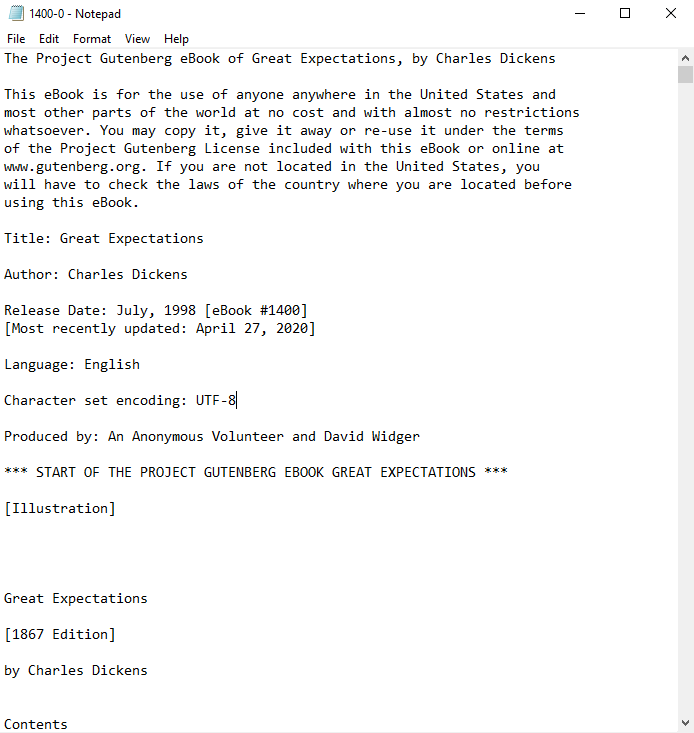
\includegraphics[width = 0.8\textwidth]{Images/data_clean_orig.PNG} % enter the filename here
		\caption{Before File Editing - Great Expectations}
		\label{fig:data-clean-orig}
	\end{center}
\end{figure}

\begin{figure}[H]
	\begin{center}
		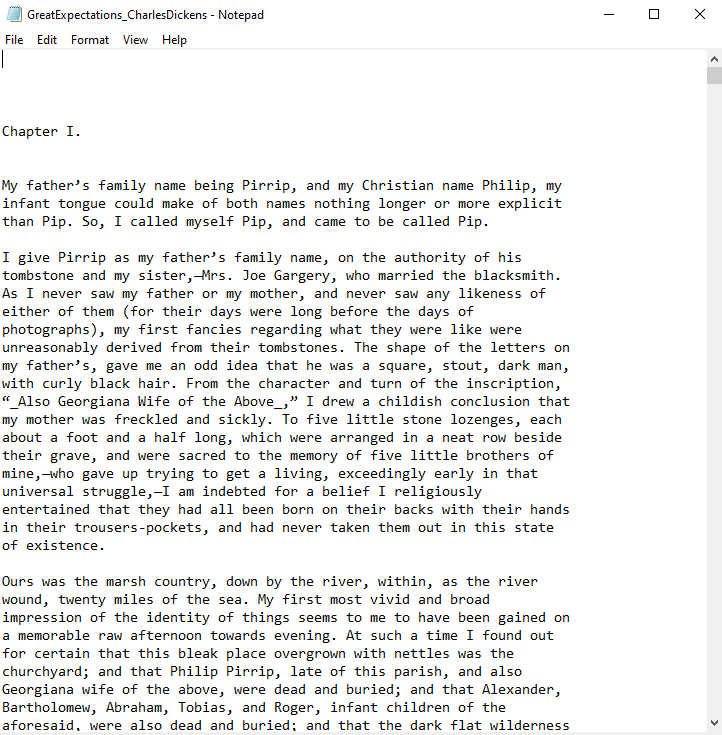
\includegraphics[width = 0.8\textwidth]{Images/data_clean_final.PNG} % enter the filename here
		\caption{After File Editing - Great Expectations}
		\label{fig:data-clean-final}
	\end{center}
\end{figure}


\subsection{Character Replacement}
\label{sec:data-clean-coding}

This is a somewhat simpler version to work with, as we perform a quick analysis of the frequency of certain outlying characters and either remove them or replace them on the basis of whether they would tentatively taint our data set, be it the training data or the testing data sets.

The way we accomplish this task is by the use of a brief Python code, which is as follows. But before we go about sharing which characters to remove or replace, let us import the right packages to accomplish this task.

\begin{code}
\label{code:libraries}
\begin{minted}[frame=single,framesep=10pt]{python}
import pandas as pd
import numpy as np
import matplotlib.pyplot as plt
import os
import math
import re
from wordcloud import WordCloud, STOPWORDS
from PIL import Image
\end{minted}
\caption{List of all libraries used in the Dissertation}
\end{code}

Next, we shall define a PATH and a list to store all the data source files in that location. This can be interchanged with the links to \textcite{project-gutenburg} as well, but that way, we would not be able to directly work with \ref{sec:data-clean-files}. From the code \ref{code:libraries}, we already have the necessary libraries imported.

\begin{code}
\label{code:data-source-location}
\begin{minted}[frame=single,framesep=10pt]{python}
PATH = '~/Dissertation/markovchain/datasets/'

all_files = os.listdir(PATH)
all_files

\end{minted}
\caption{A sample location where the data sets are being stored}
\end{code}

Finally, let us understand which characters were causing problems through the next piece of code.


\begin{code}
\label{code:data-clean}
\begin{minted}[frame=single,framesep=10pt]{python}
def data_cleaning(novel):
    
    novel = re.sub('\n', ' ', novel)
    novel = re.sub('_', ' ', novel)
    novel = re.sub('\u200a', ' ', novel)
    novel = re.sub('½', '1/2', novel)
    novel = re.sub(' +', ' ', novel)
    novel = re.sub('\t', ' ', novel)
    novel = re.sub('…', ' ', novel)
    
    return novel

\end{minted}
\caption{The characters +, \textunderscore, $\cdots$ mentioned above cause a little problem, bringing some sort of ambiguity for the same novel in the final data model. Thus, we end up replacing them}.
\end{code}


\section{List of Novels} % enter the name of the section here
\label{sec:novels-list} % enter the section label here (for cross-referencing)

Before sharing the actual word clouds, let us consider the code we shall be using for this purpose. We use the code from \ref{code:data-source-location} in order to edit out all the unnecessary characters.

\begin{code}
\label{code:word-cloud}
\begin{minted}[frame=single,framesep=10pt]{python}
for file in all_files:
            
    book = open(PATH + file, 'r', encoding = 'utf-8-sig')
    novel = book.read()
    
    novel = re.sub('\n', ' ', novel)
    novel = re.sub('_', ' ', novel)
    novel = re.sub('\u200a', ' ', novel)
    novel = re.sub('½', '1/2', novel)
    novel = re.sub(' +', ' ', novel)
    novel = re.sub('\t', ' ', novel)
    novel = re.sub('…', ' ', novel)
    
    word_cloud = WordCloud(
        width=3000,
        height=2000,
        random_state=123,
        max_words=100,
        background_color="purple",
        colormap="Set2",
        collocations=False,
        stopwords=STOPWORDS
    ).generate(novel)
    
    word_cloud.to_file(f'{file[:-4]}.jpeg')
    
\end{minted}
\caption{The characters +, \textunderscore, $\cdots$ mentioned above cause a little problem, bringing some sort of ambiguity for the same novel in the final data model. Thus, we end up replacing them}.
\end{code}

\begin{code}
\label{code:histograms}
\begin{minted}[frame=single,framesep=10pt]{python}
for file in all_files:
    
    dflux = charslen_df[file]
    dflux2 = charslen_df[file].loc[charslen_df[file] < 10000]
    dflux3 = charslen_df[file].loc[charslen_df[file] < 1000]
    dflux4 = charslen_df[file].loc[charslen_df[file] < 100]


    fig, axes = plt.subplots(1, 4)
    plt.rcParams["figure.figsize"] = (20,4)
    plt.title(f'{file[:-4]}')

    dflux.hist(bins=10, ax=axes[0])
    dflux2.hist(bins=10, ax=axes[1])
    dflux3.hist(bins=10, ax=axes[2])
    dflux4.hist(bins=10, ax=axes[3])
    
    plt.savefig(f'char_hist_{file[:-4]}.jpeg', bbox_inches='tight')
    
\end{minted}
\caption{All of our histograms are being divided into 4 slicings for a better understanding of the character frequencies}.
\end{code}

We are using 8 novels in our Natural Language Processing model, which heavily relies on character analysis. A list of the books we use is as follows:

\begin{itemize}
    \item \textcite{great_expectations}
    \item \textcite{great-gatsby}
    \item \textcite{huckleberry-finn}
    \item \textcite{moby-dick}
    \item \textcite{pride-prejudice}
    \item \textcite{sherlock-holmes}
    \item \textcite{sign-of-the-four}
    \item \textcite{oliver-twist}
\end{itemize}

We created some word clouds for each book, and we shall briefly go over a short summary of each novel. One key thing to note is all these novels are available for reading widely. Their publishing rights have lapsed since the year mentioned next to each novel and are available in the public domain for anyone to read.

Additionally, we have also created some character occurrence frequencies, varying from the complete dataset to certain sections of them. They would be available in the images following the word clouds. Let us also look at just one example of a Histogram for character frequencies in this novel. Here, we are working with character frequencies in 4 stages.

\begin{itemize}
    \item \textbf{Complete Frequency}
    \item \textbf{Frequency $<$ 10000 in occurrence}
    \item \textbf{Frequency $<$ 1000 in occurrence}
    \item \textbf{Frequency $<$ 100 in occurrence}
\end{itemize}
 
\subsection{\textcite{great_expectations}} %enter the name of the subsection here
\label{sec:great-expectations} % enter the subsection label here (for cross-referencing)

Great Expectations follows the childhood and young adult years of Pip a blacksmith's apprentice in a country village. He suddenly comes into a large fortune (his great expectations) from a mysterious benefactor and moves to London where he enters high society. He thinks he knows where the money has come from but he turns out to be sadly mistaken. The story also follows Pip's dealings with Estella, a young woman he adores but who cannot return his love. \textcite{great_expectations-summary}. Below is a quick word cloud from the complete book. 

\begin{figure}[H]
	\begin{center}
		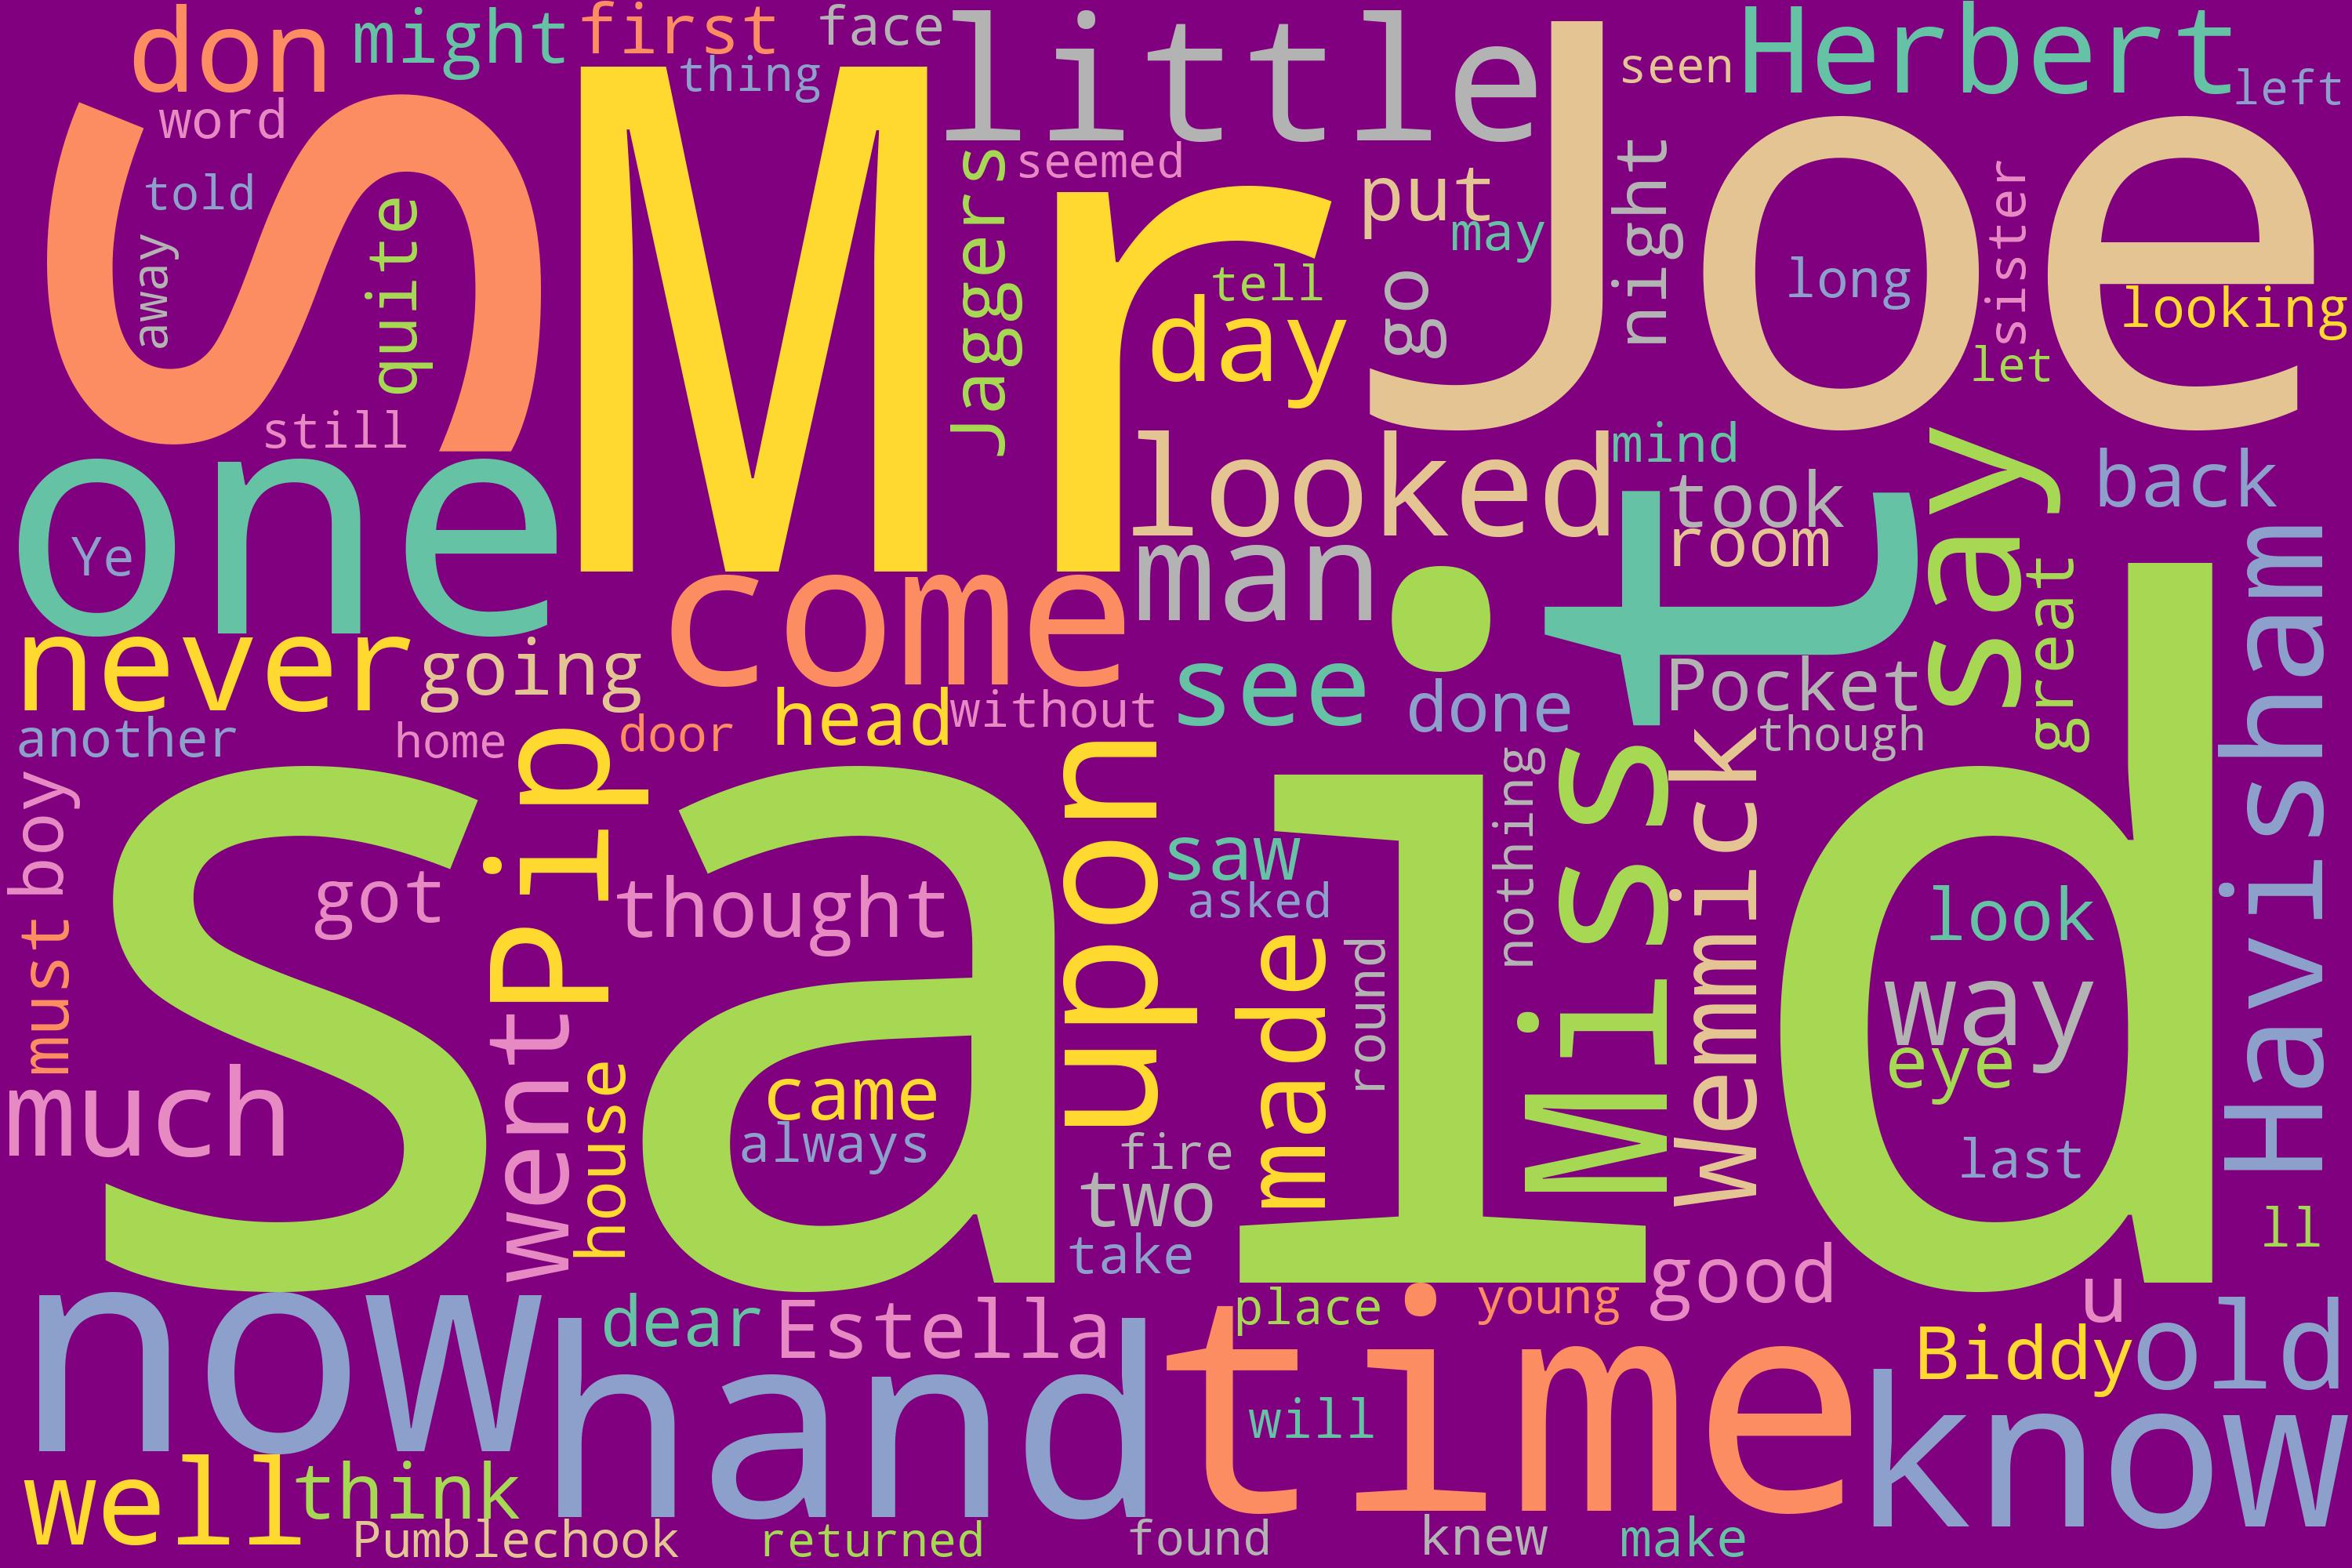
\includegraphics[width = 0.7\textwidth]{Images/GreatExpectations_CharlesDickens.jpeg} % enter the filename here
		\caption{Word Cloud - Great Expectations}
		\label{fig:great-expectations}
	\end{center}
\end{figure}

In Great Expectations, we do see Pip, who is a very prominent character in the book, along with his counterpart, Estella.

\begin{figure}[H]
	\begin{center}
		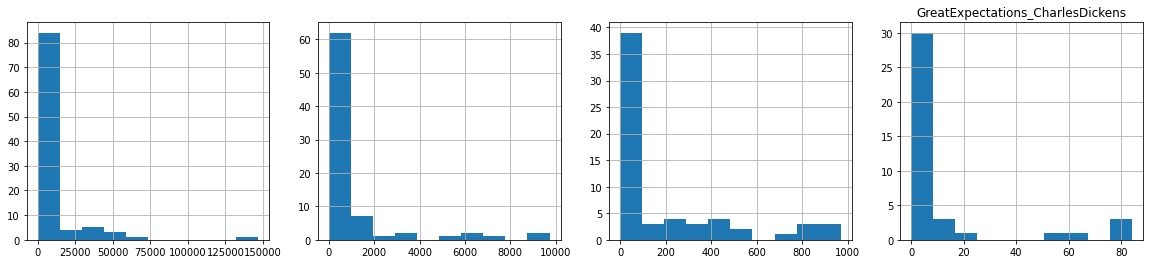
\includegraphics[width = 1.0\textwidth]{Images/char_hist_GreatExpectations_CharlesDickens.jpeg} % enter the filename here
		\caption{Character Histogram - Great Expectations}
		\label{fig:histogram-greatexp}
	\end{center}
\end{figure}

\subsection{\textcite{great-gatsby}} %enter the name of the subsection here
\label{sec:great-gatsby} % enter the subsection label here (for cross-referencing)

F. Scott Fitzgerald's novel, The Great Gatsby, follows Jay Gatsby, a man who orders his life around one desire: to be reunited with Daisy Buchanan, the love he lost five years earlier. Gatsby's quest leads him from poverty to wealth, into the arms of his beloved, and eventually to death. Published in 1925, The Great Gatsby is a classic piece of American fiction. It is a novel of triumph and tragedy, noted for the remarkable way Fitzgerald captured a cross-section of American society. \textcite{great-gatsby-summary}. Below is a quick word cloud from the complete book. 

\begin{figure}[H]
	\begin{center}
		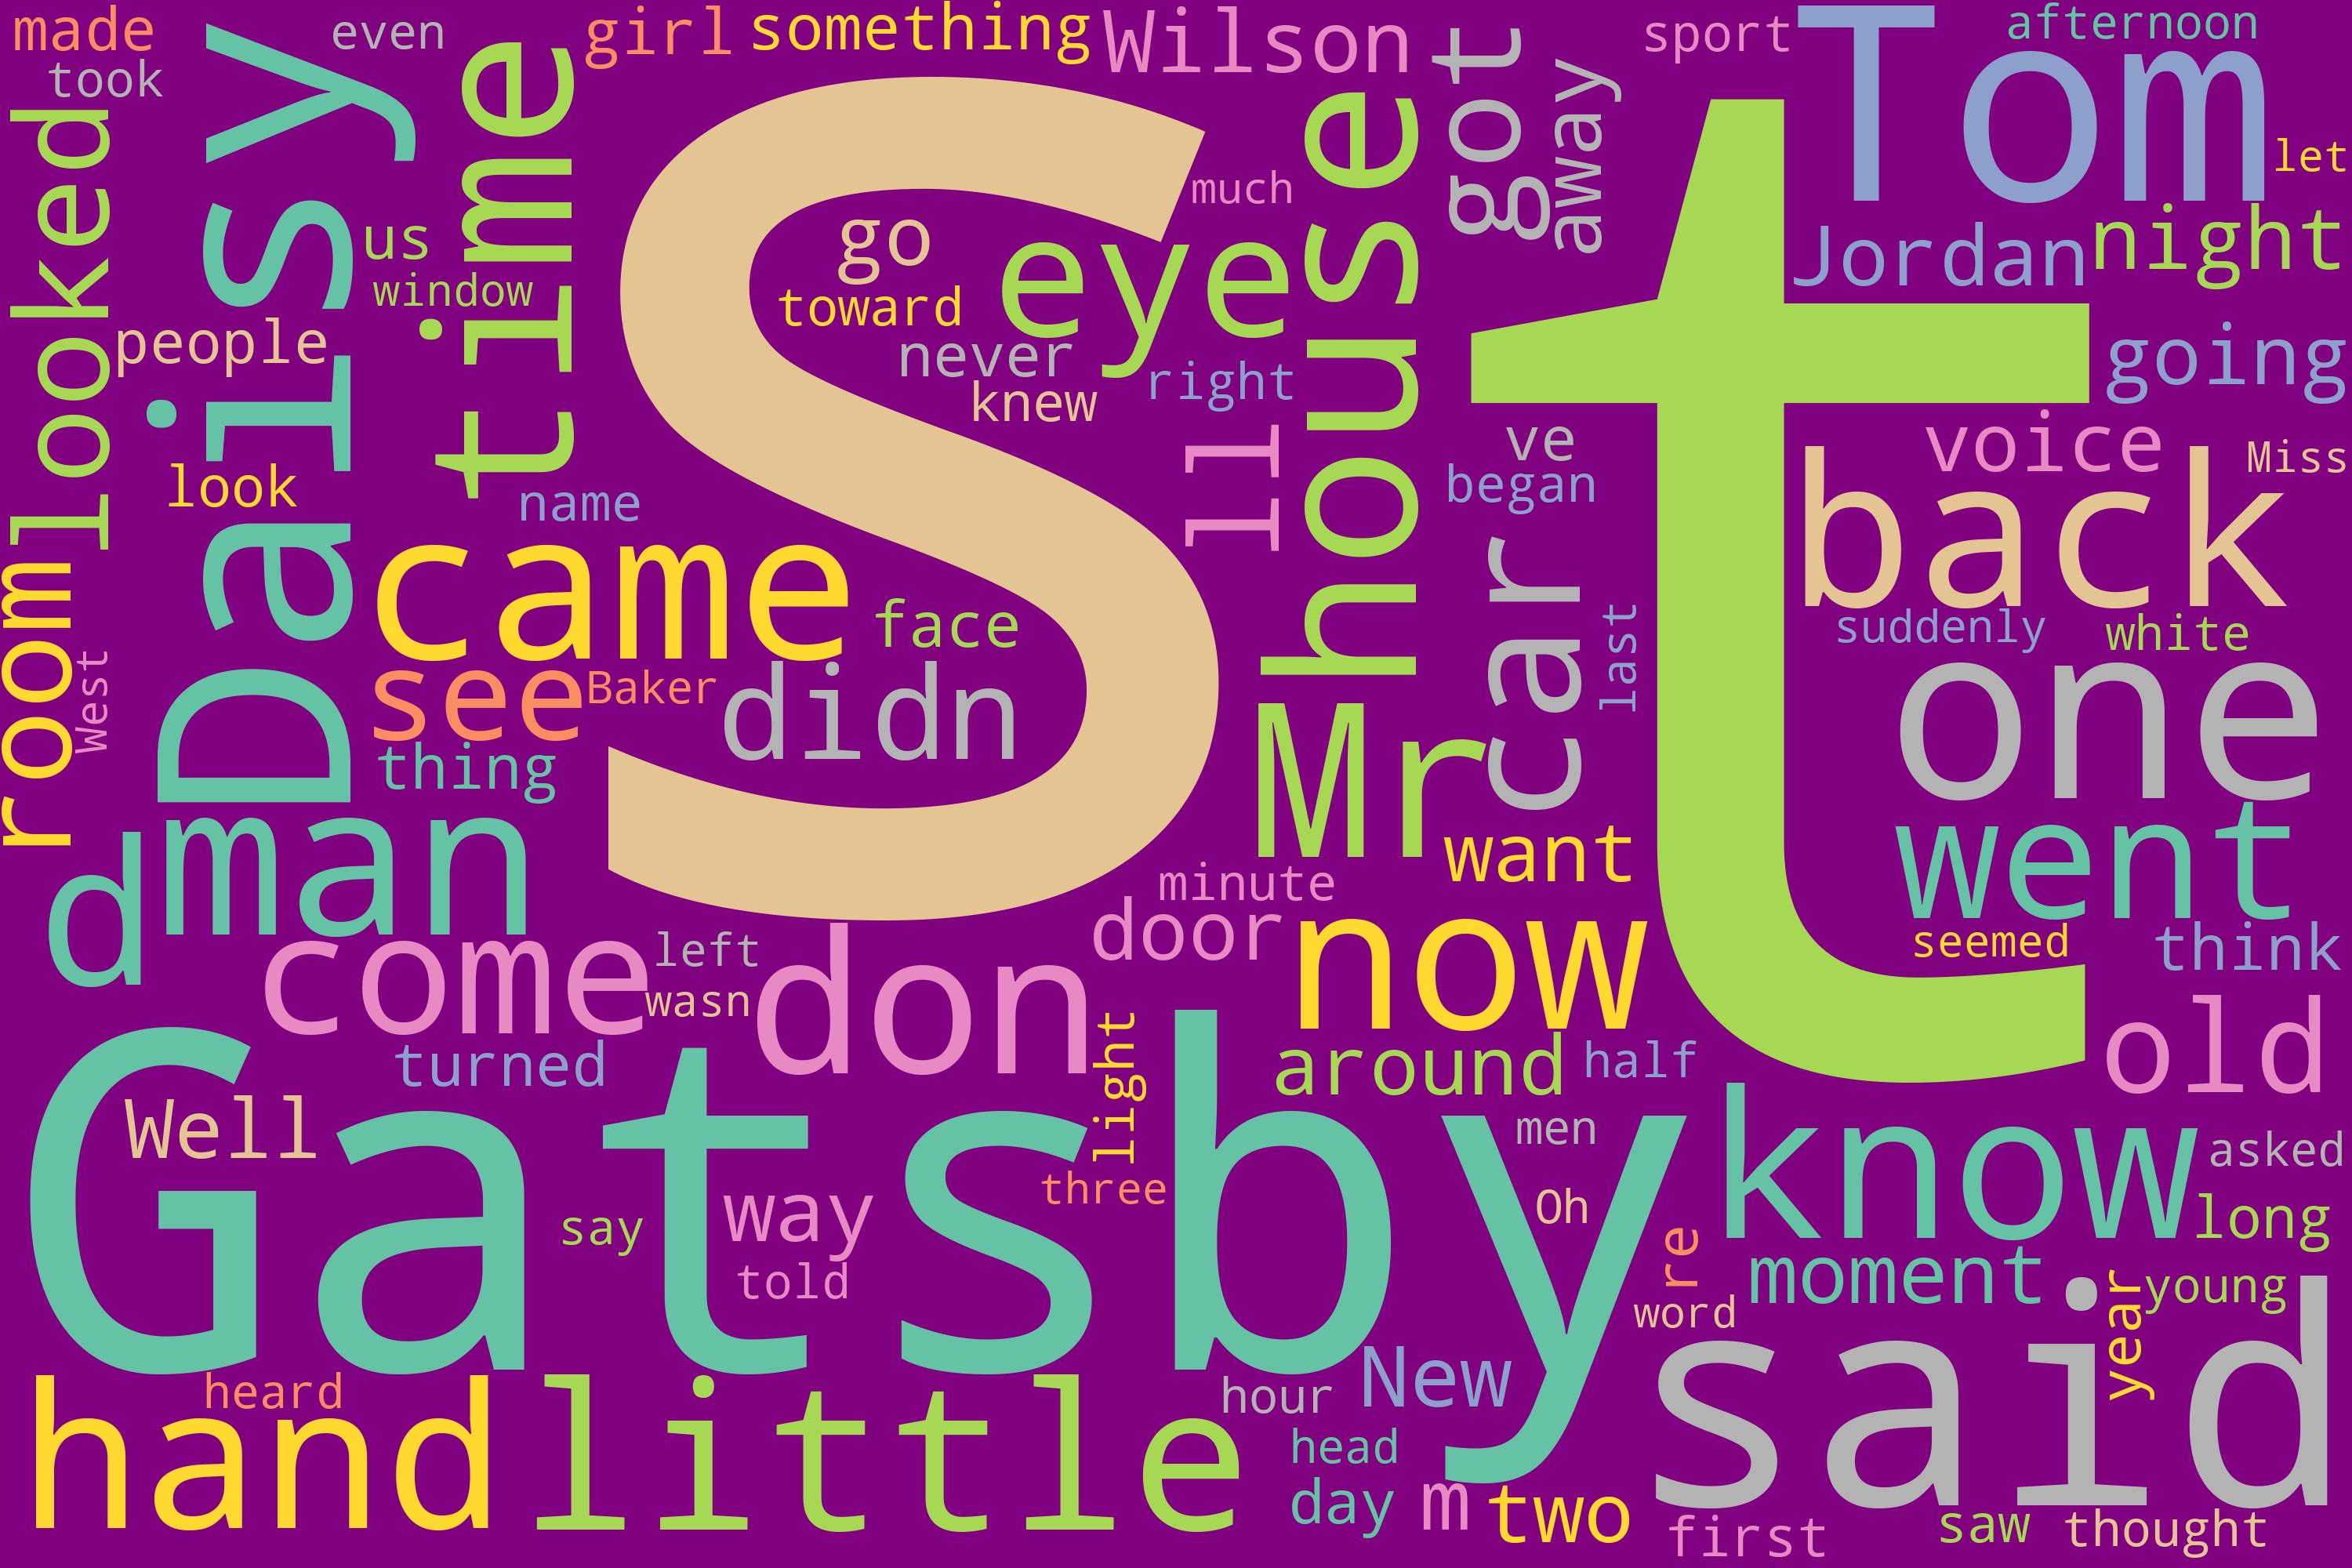
\includegraphics[width = 0.7\textwidth]{Images/GreatGatsby_FScottFitzgerald.jpeg} % enter the filename here
		\caption{Word Cloud - Great Gatsby}
		\label{fig:great-gatsby}
	\end{center}
\end{figure}

\begin{figure}[H]
	\begin{center}
		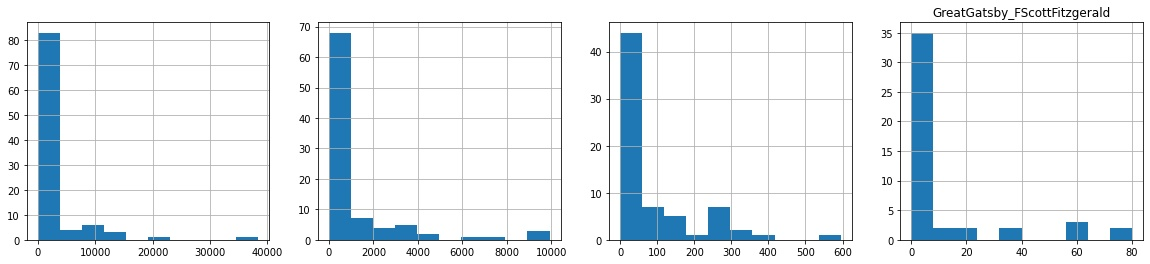
\includegraphics[width = 1.0\textwidth]{Images/char_hist_GreatGatsby_FScottFitzgerald.jpeg} % enter the filename here
		\caption{Character Histogram - Great Gatsby}
		\label{fig:histogram-greatgatsby}
	\end{center}
\end{figure}


\subsection{\textcite{huckleberry-finn}} %enter the name of the subsection here
\label{sec:huckleberry-finn} % enter the subsection label here (for cross referencing)

The book’s narrator is Huckleberry Finn, a youngster whose artless vernacular speech is admirably adapted to detailed and poetic descriptions of scenes, vivid representations of characters, and narrative renditions that are both broadly comic and subtly ironic. The book’s pages are dotted with idyllic descriptions of a great river and the surrounding forests, Huck’s good nature, and unconscious humor. But a thread that runs through adventure after the adventure is that of human cruelty, which shows itself both in the acts of individuals and in their unthinking acceptance of such institutions as slavery. \textcite{huckleberry-finn-summary}. Below is a quick word cloud from the complete book. 

\begin{figure}[H]
	\begin{center}
		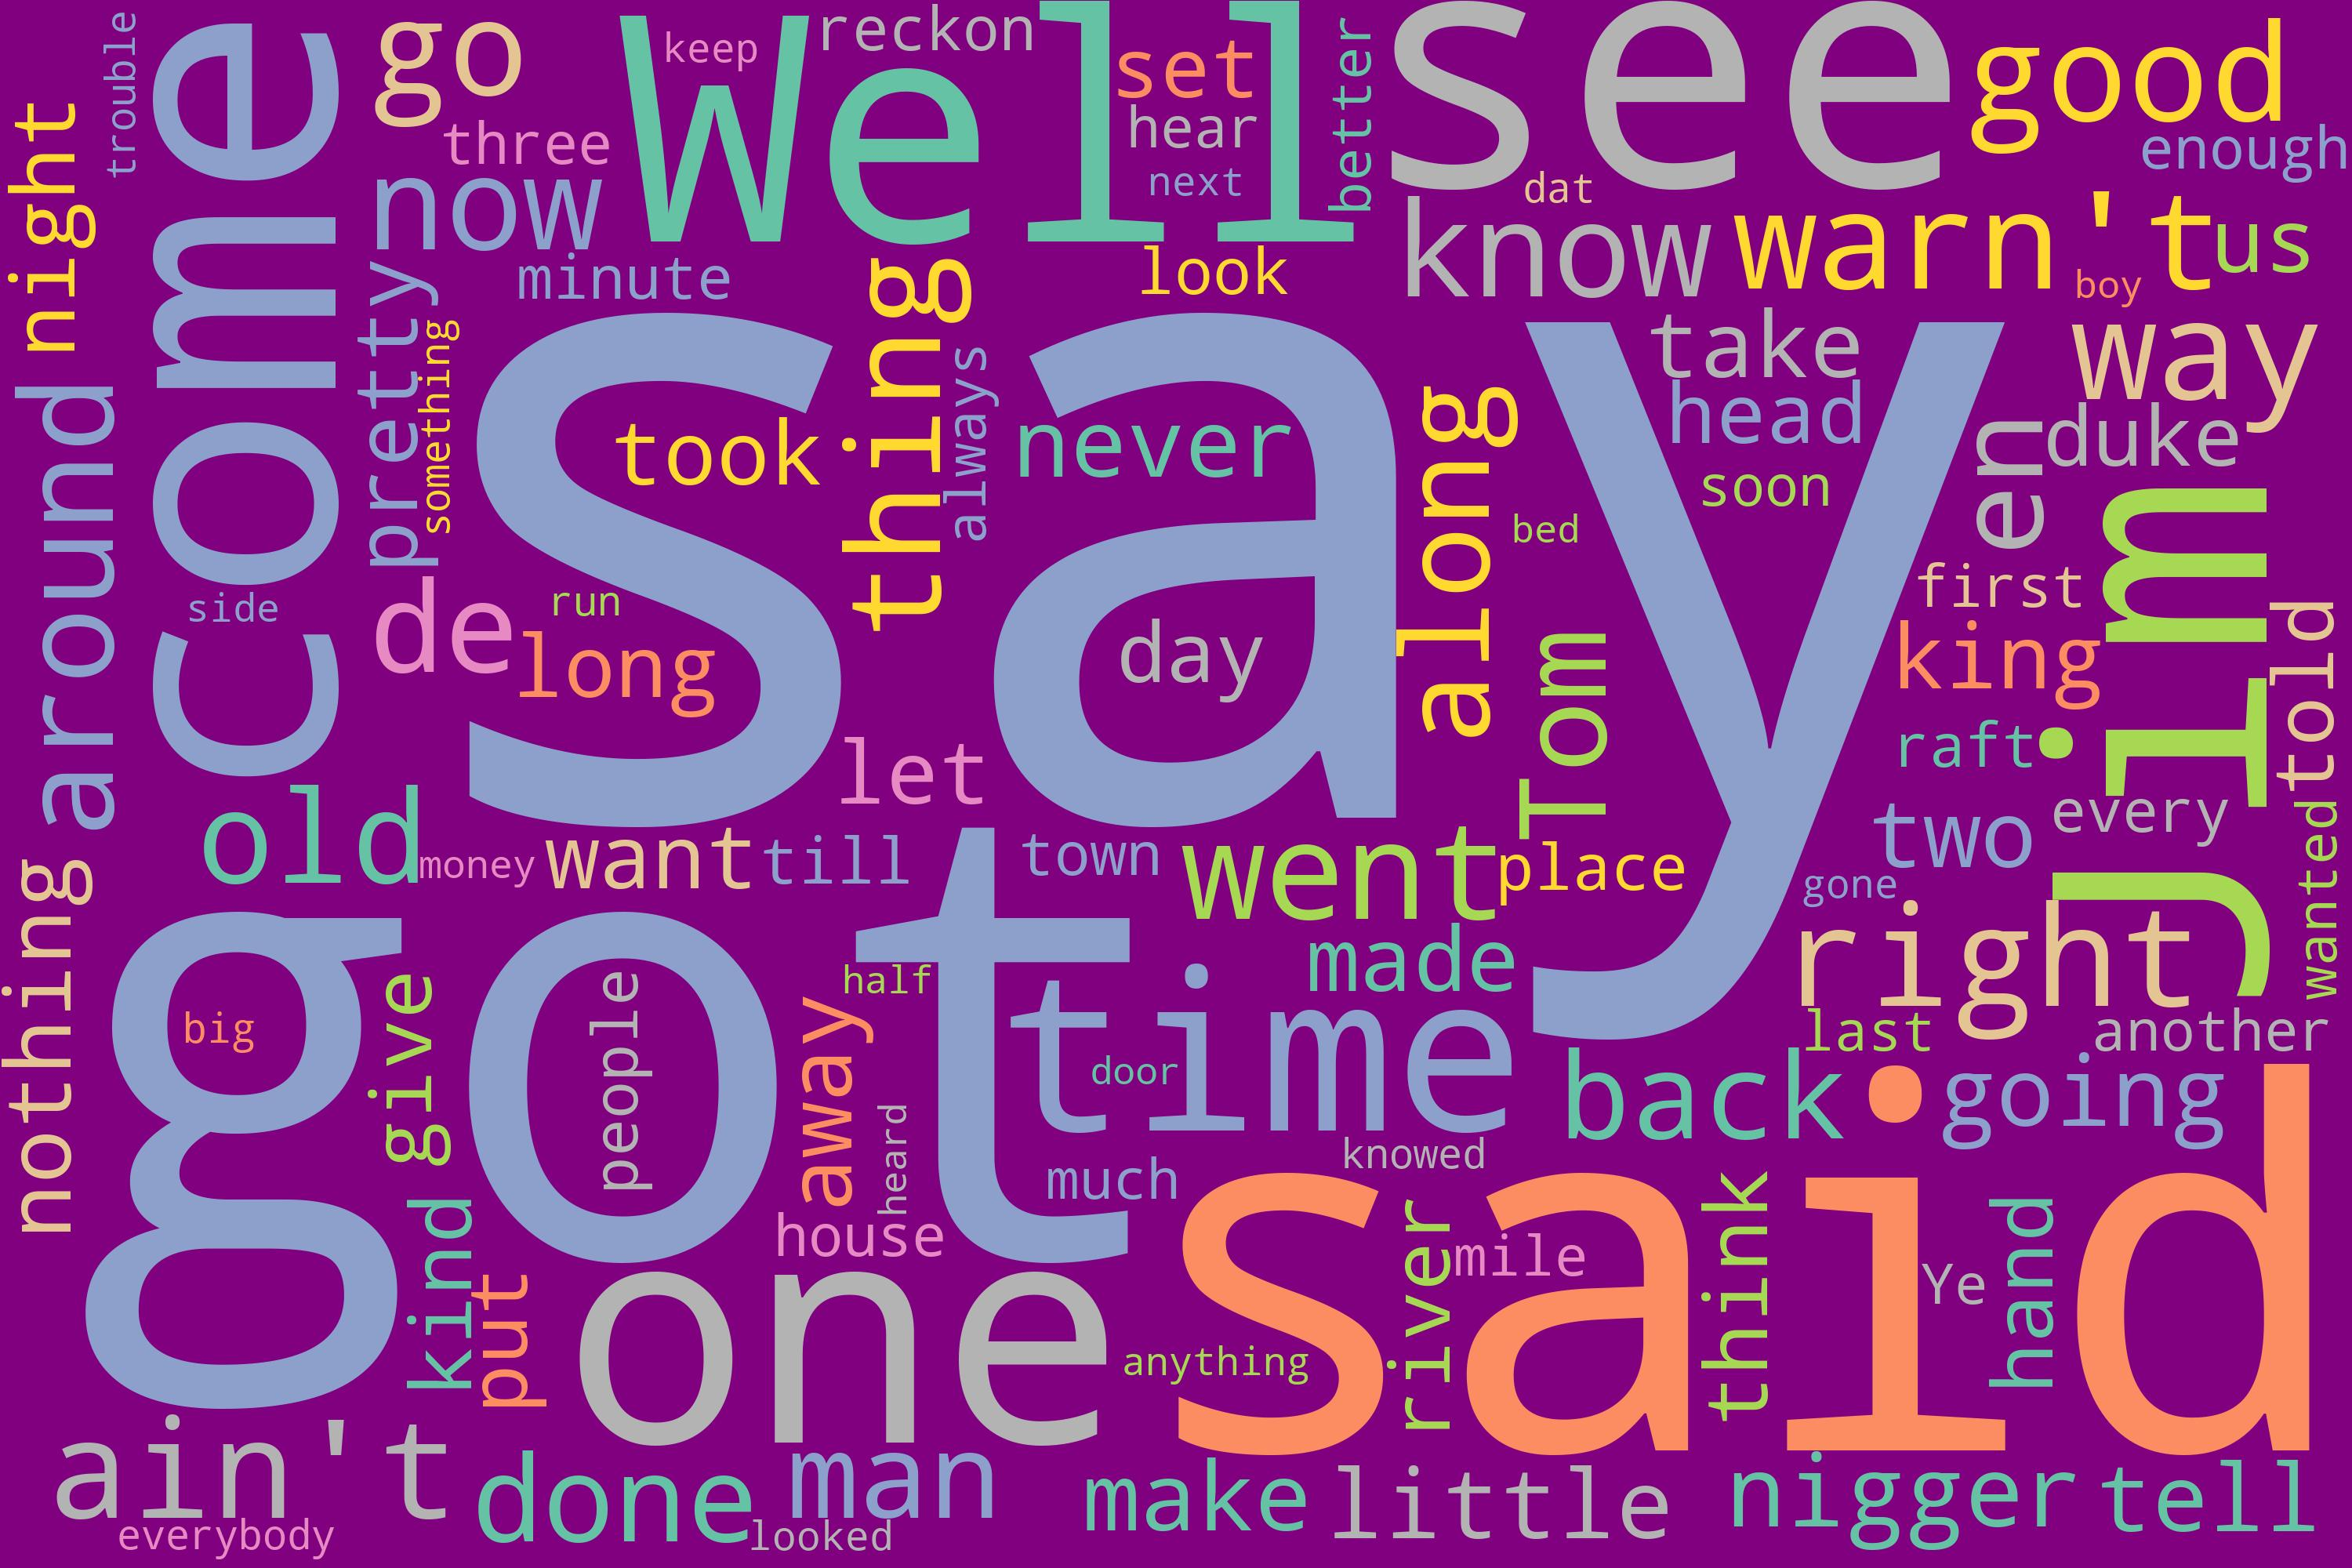
\includegraphics[width = 0.7\textwidth]{Images/HuckleberryFinn_MarkTwain.jpeg} % enter the filename here
		\caption{Word Cloud - Huckleberry Finn}
		\label{fig:huckleberry-finn}
	\end{center}
\end{figure}

\begin{figure}[H]
	\begin{center}
		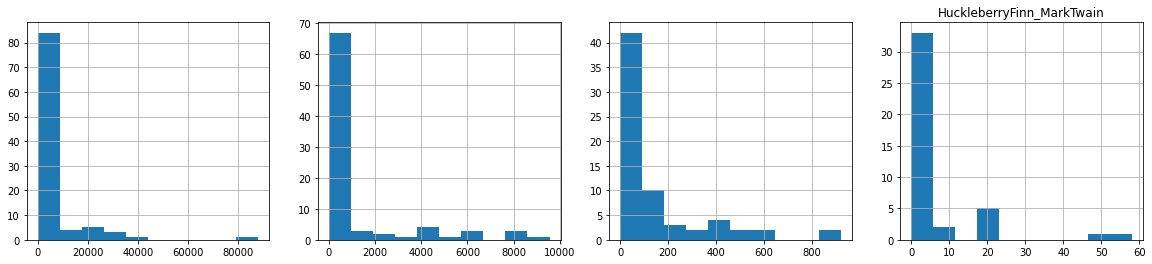
\includegraphics[width = 1.0\textwidth]{Images/char_hist_HuckleberryFinn_MarkTwain.jpeg} % enter the filename here
		\caption{Character Histogram - Huckleberry Finn}
		\label{fig:histogram-huckbfinn}
	\end{center}
\end{figure}

\subsection{\textcite{moby-dick}} %enter the name of the subsection here
\label{sec:moby-dick} % enter the subsection label here (for cross referencing)

Moby Dick famously begins with the narratorial invocation “Call me Ishmael.” The narrator, like his biblical counterpart, is an outcast. Ishmael, who turns to the sea for meaning, relays to the audience the final voyage of the Pequod, a whaling vessel. Amid a story of tribulation, beauty, and madness, the reader is introduced to a number of characters, many of whom have names with religious resonance. Moby Dick can sustain numerous, if not seemingly infinite, readings generated by multiple interpretative approaches. One of the most fruitful ways to appreciate the novel’s complexity is through the names that Melville gave to its characters, many of which are shared with figures of the Abrahamic religions. \textcite{moby-dick-summary}. Below is a quick word cloud from the complete book. 

\begin{figure}[H]
	\begin{center}
		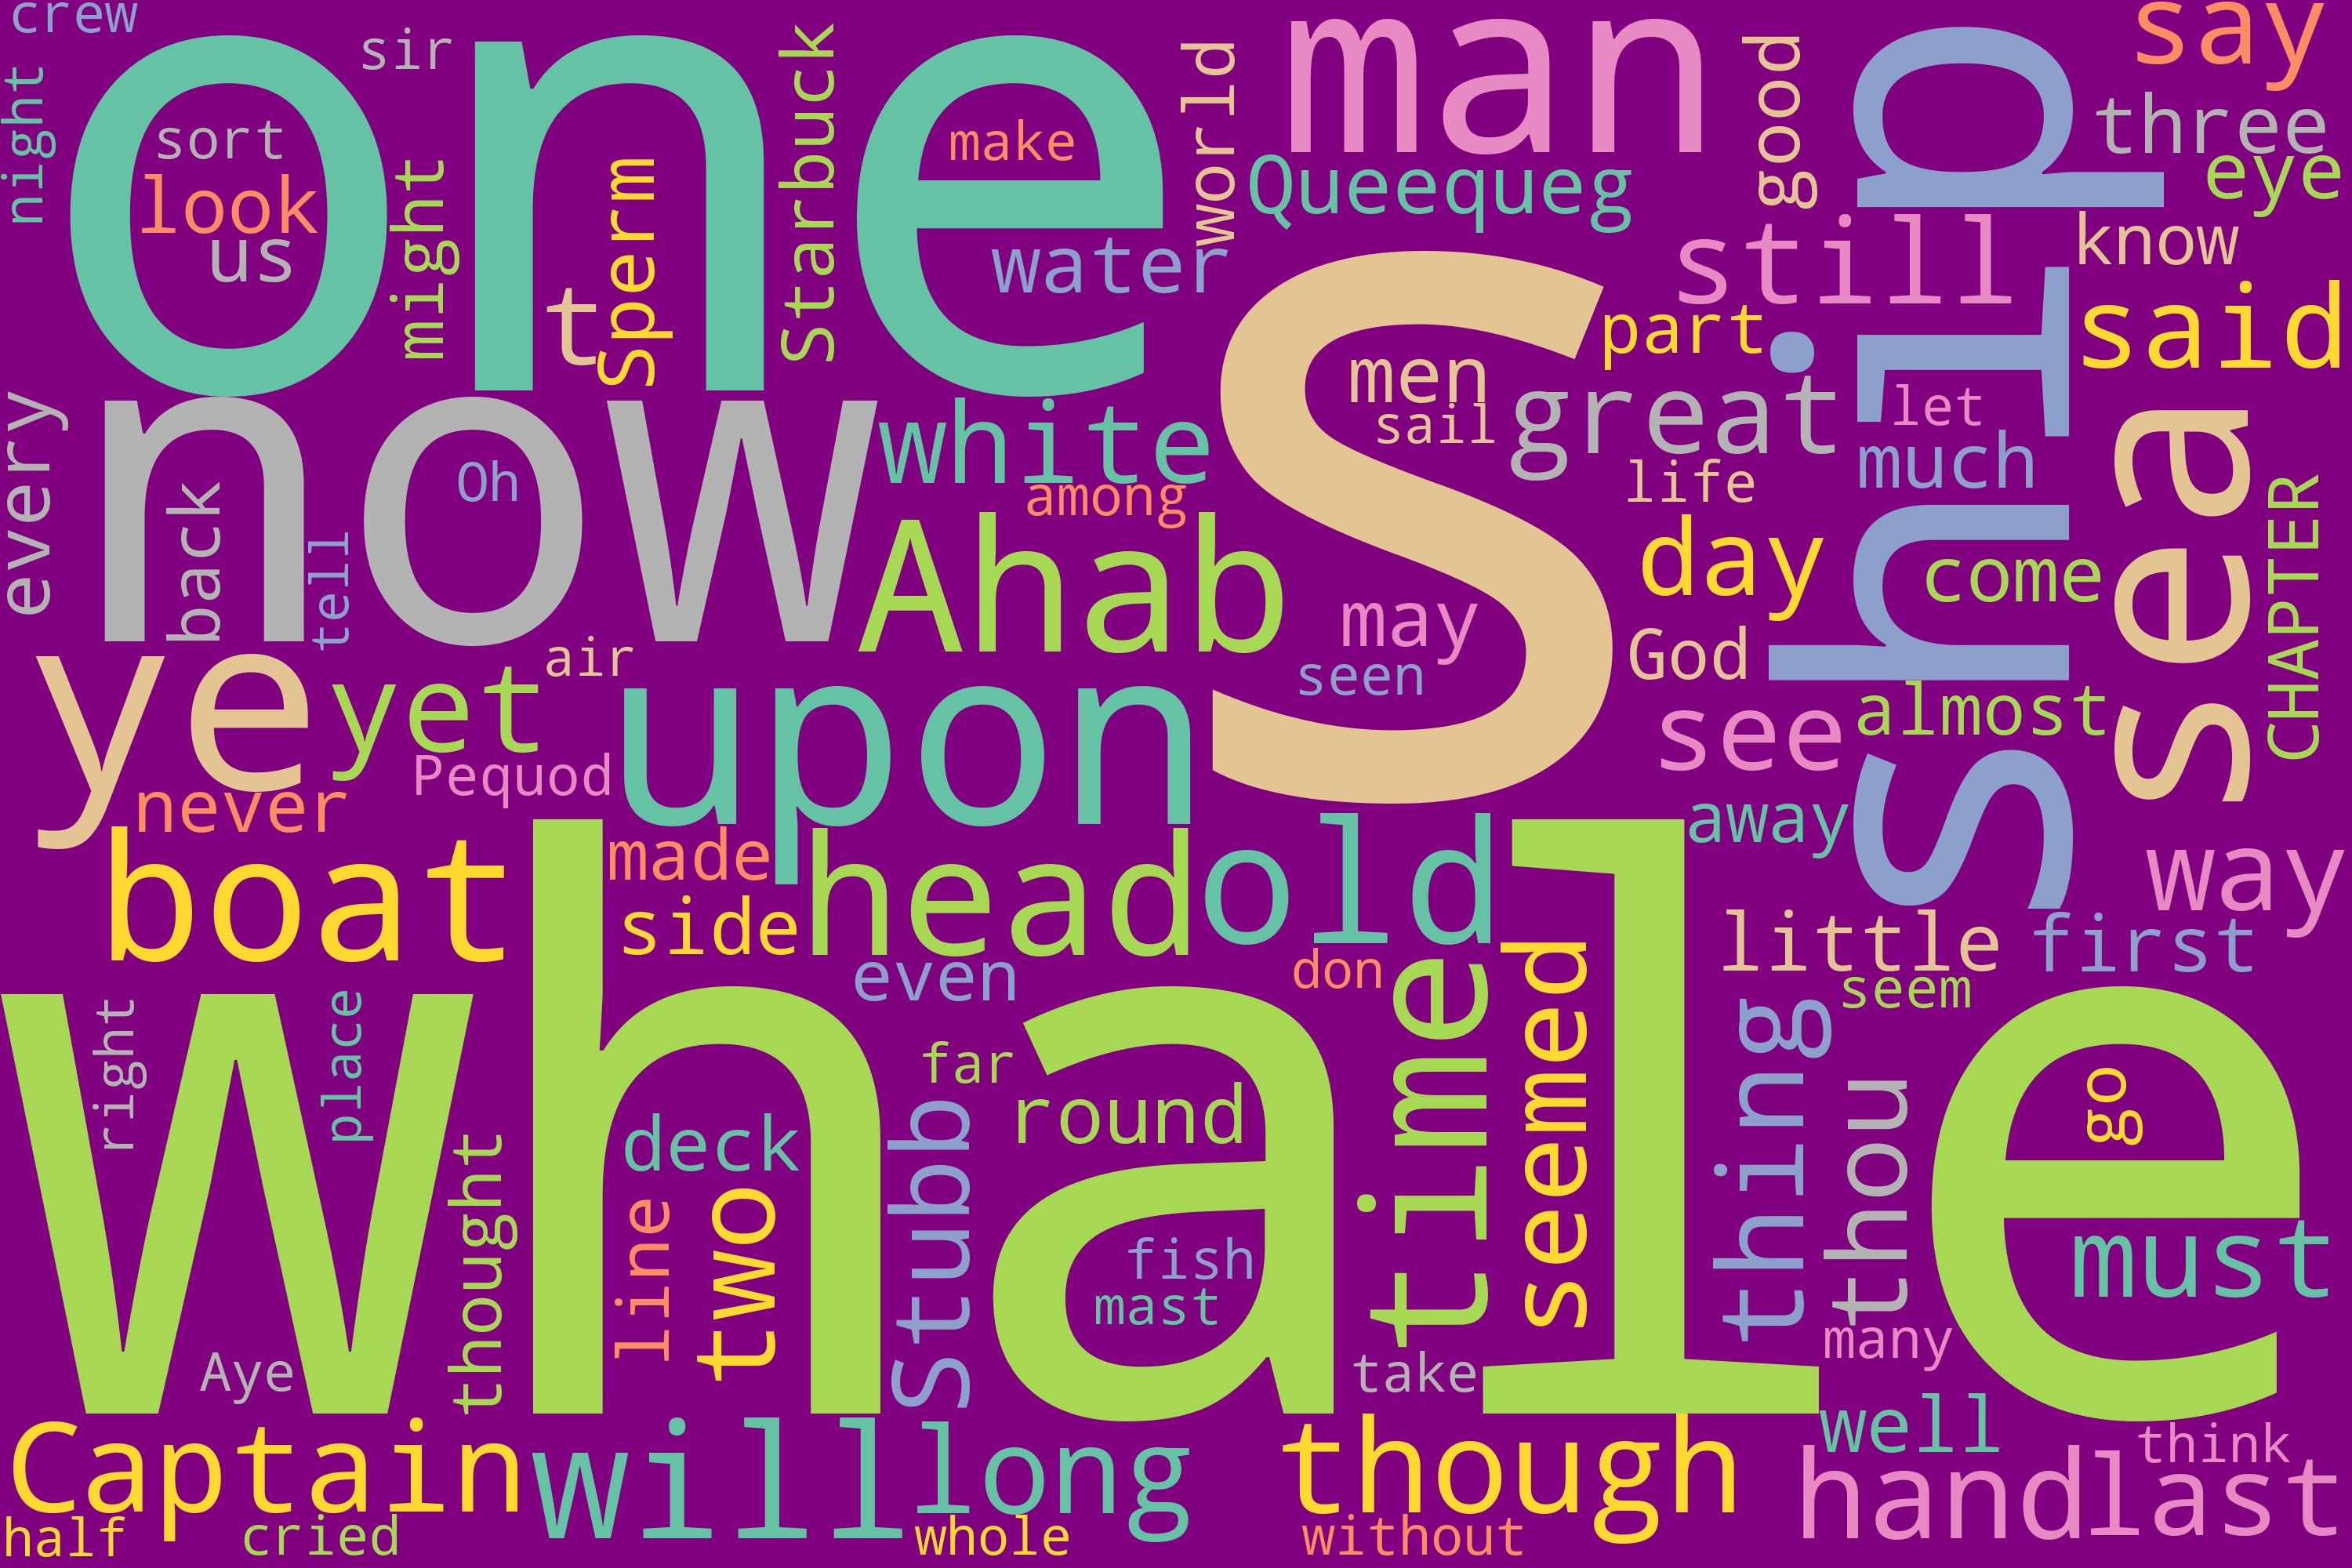
\includegraphics[width = 0.7\textwidth]{Images/MobyDick_HermanMelville.jpeg} % enter the filename here
		\caption{Word Cloud - Moby Dick}
		\label{fig:moby-dick}
	\end{center}
\end{figure}

\begin{figure}[H]
	\begin{center}
		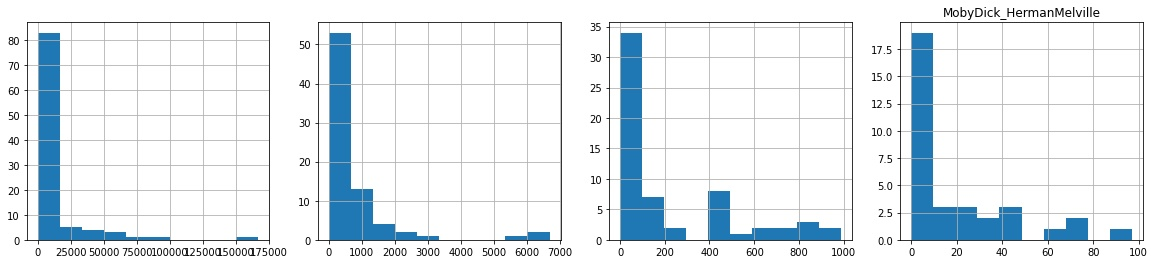
\includegraphics[width = 1.0\textwidth]{Images/char_hist_MobyDick_HermanMelville.jpeg} % enter the filename here
		\caption{Character Histogram - Moby Dick}
		\label{fig:histogram-mobydick}
	\end{center}
\end{figure}


\subsection{\textcite{oliver-twist}} %enter the name of the subsection here
\label{sec:oliver-twist} % enter the subsection label here (for cross referencing)

The novel follows the journey of the titular character, Oliver Twist. Oliver, an orphan since birth, spends much of his childhood at a “child farm” (orphanage) with too many children and too little food. The farm is located roughly 70 miles outside London. Charles Dickens was well versed in the poverty of London, as he himself was a child worker after his father was sent to debtors’ prison. His appreciation of the hardships endured by impoverished citizens stayed with him for the rest of his life and was evident in his journalistic writings and novels. \textcite{oliver-twist-summary}. Below is a quick word cloud from the complete book. 

\begin{figure}[H]
	\begin{center}
		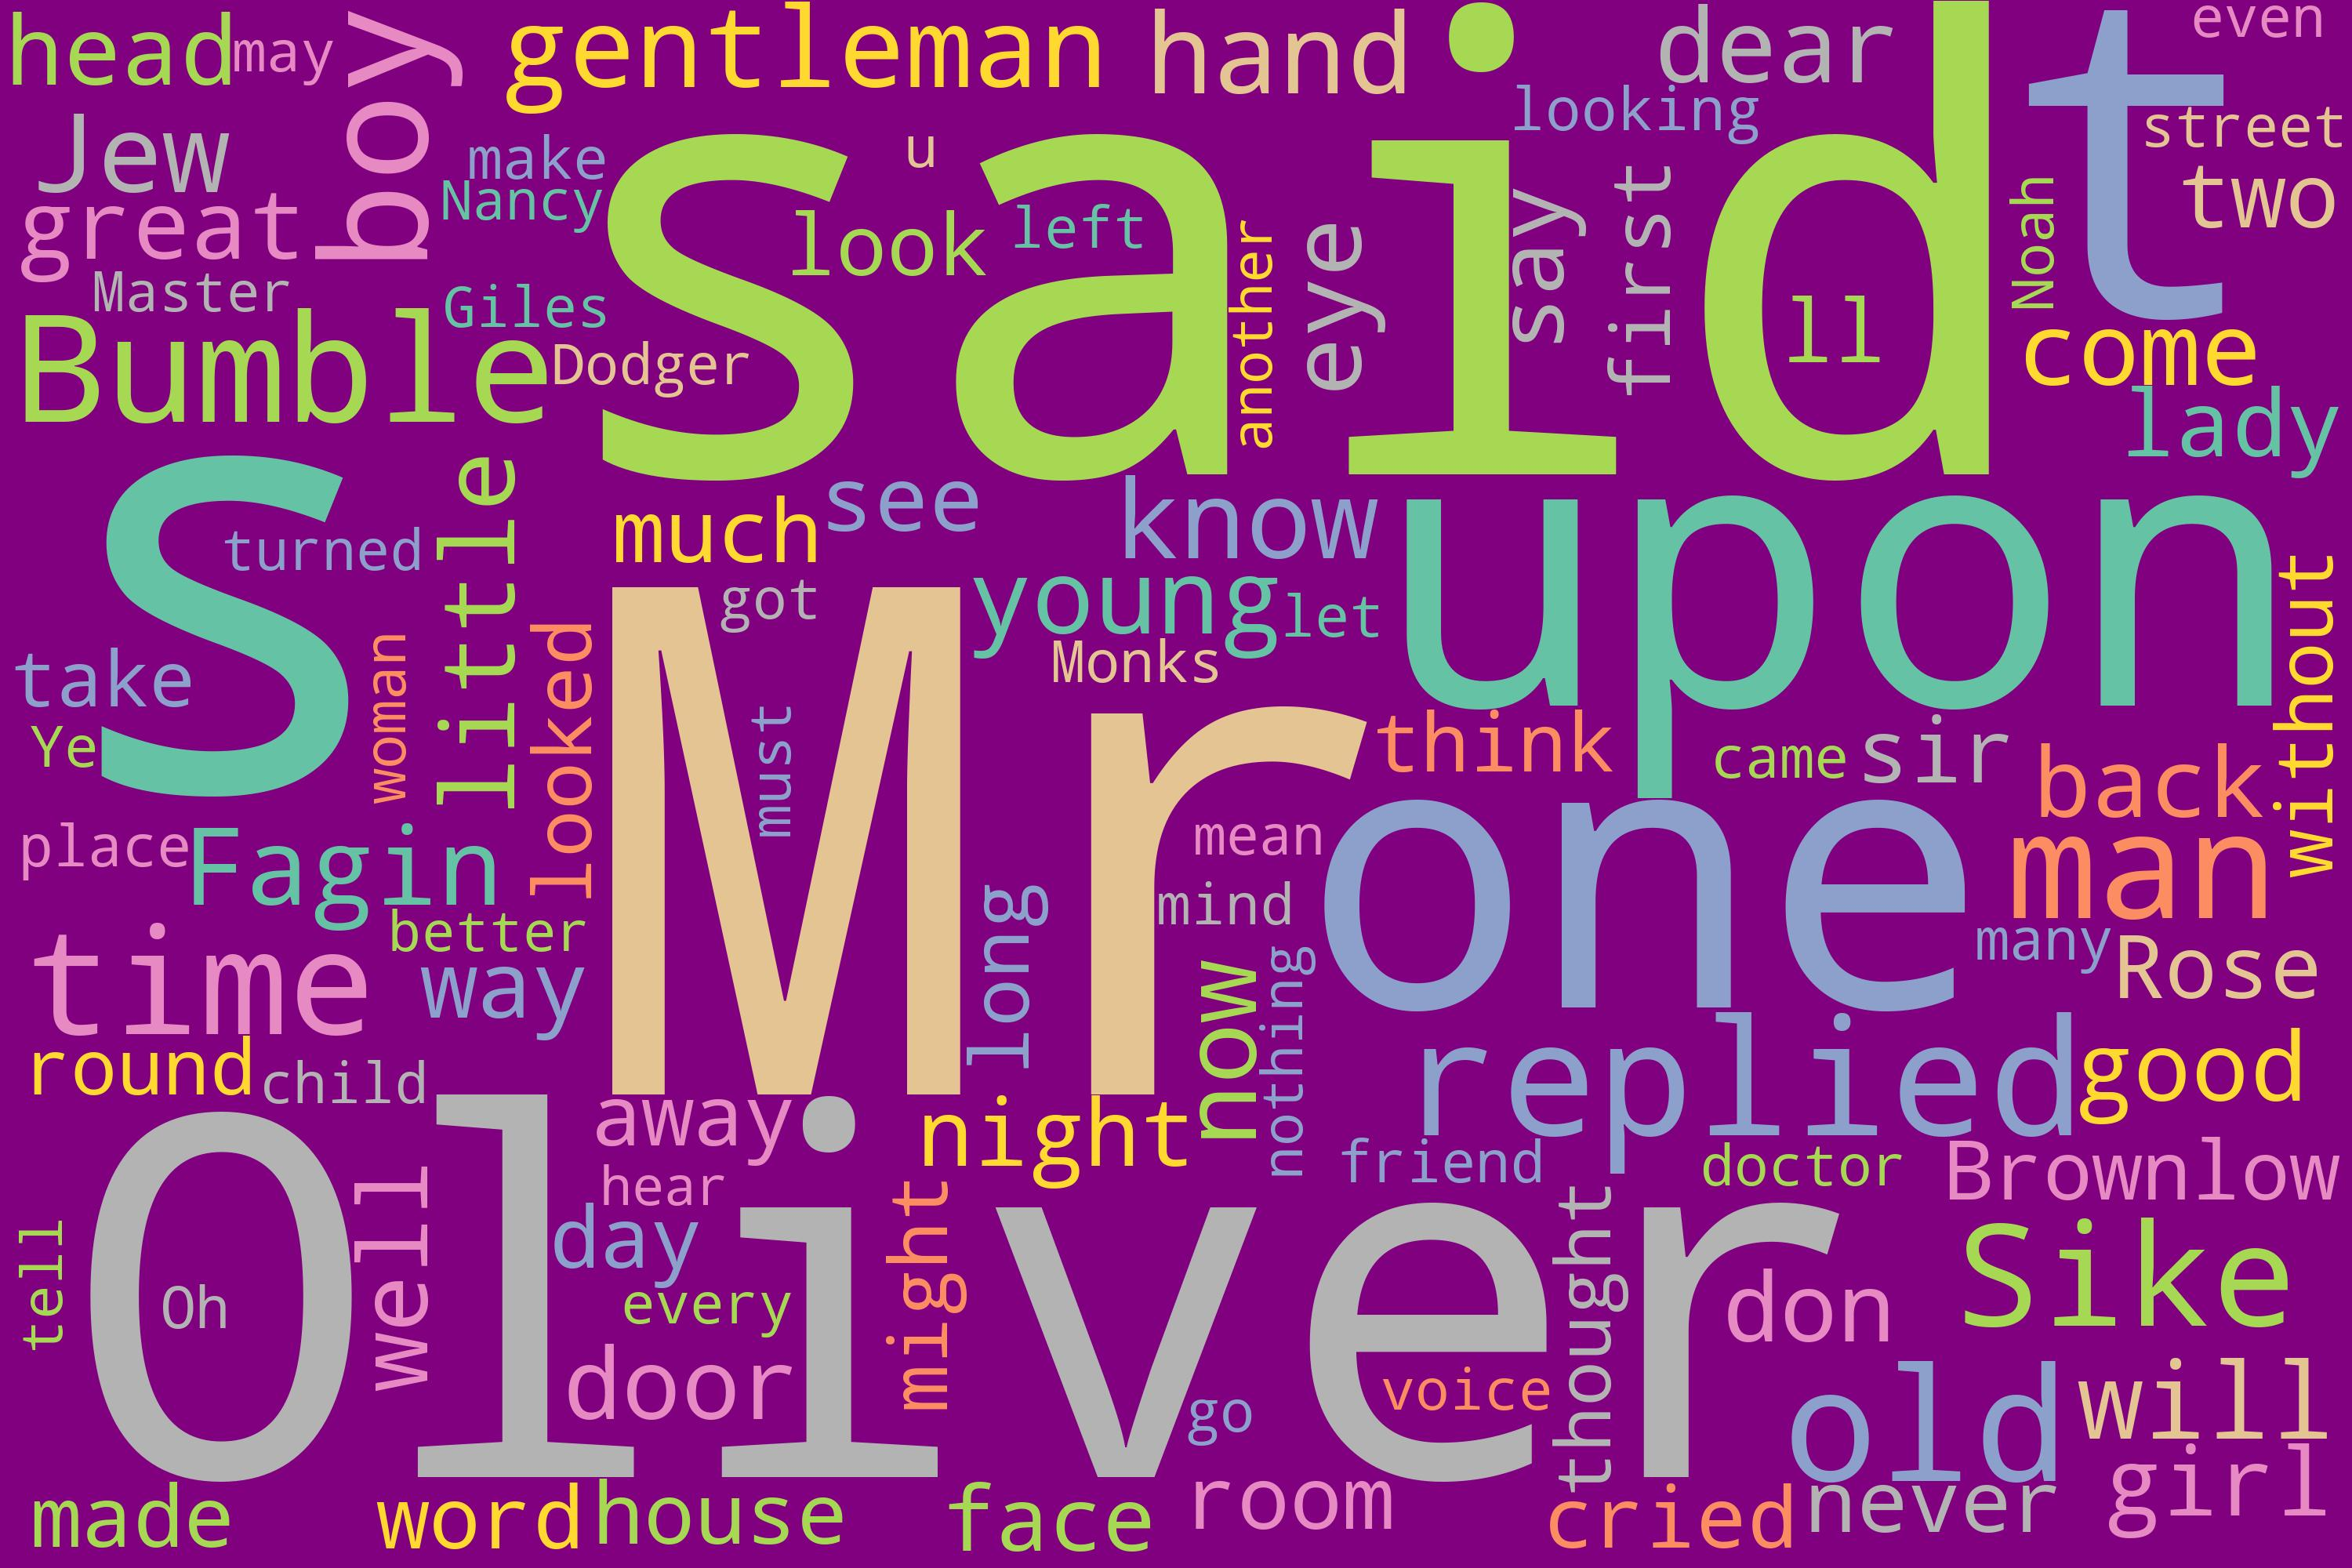
\includegraphics[width = 0.7\textwidth]{Images/OliverTwist_CharlesDickens.jpeg} % enter the filename here
		\caption{Word Cloud - Oliver Twist}
		\label{fig:oliver-twist}
	\end{center}
\end{figure}

\begin{figure}[H]
	\begin{center}
		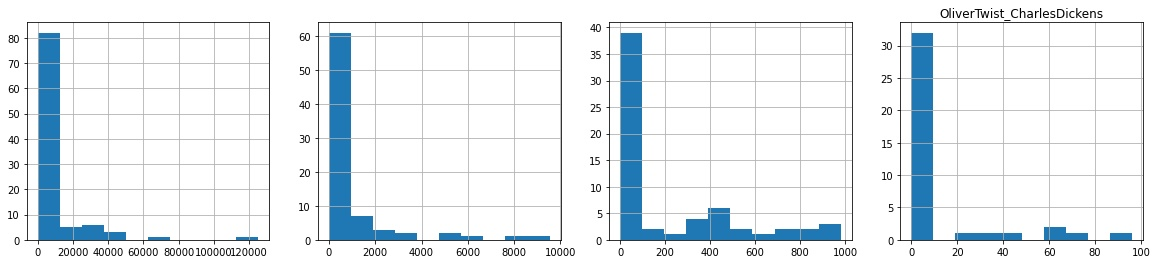
\includegraphics[width = 1.0\textwidth]{Images/char_hist_OliverTwist_CharlesDickens.jpeg} % enter the filename here
		\caption{Character Histogram - Oliver Twist}
		\label{fig:histogram-olivertwist}
	\end{center}
\end{figure}


\subsection{\textcite{pride-prejudice}} %enter the name of the subsection here
\label{sec:pride-prejudice} % enter the subsection label here (for cross referencing)

Pride and Prejudice is set in rural England at the turn of the 19th century, and it follows the Bennet family, which includes five very different sisters. The novel opens with one of the most famous lines in English literature: “It is a truth universally acknowledged, that a single man in possession of a good fortune, must be in want of a wife.” The work, which Austen initially titled First Impressions, is the second of four novels that Austen published during her lifetime. \textcite{pride-prejudice-summary}. Below is a quick word cloud from the complete book. 

\begin{figure}[H]
	\begin{center}
		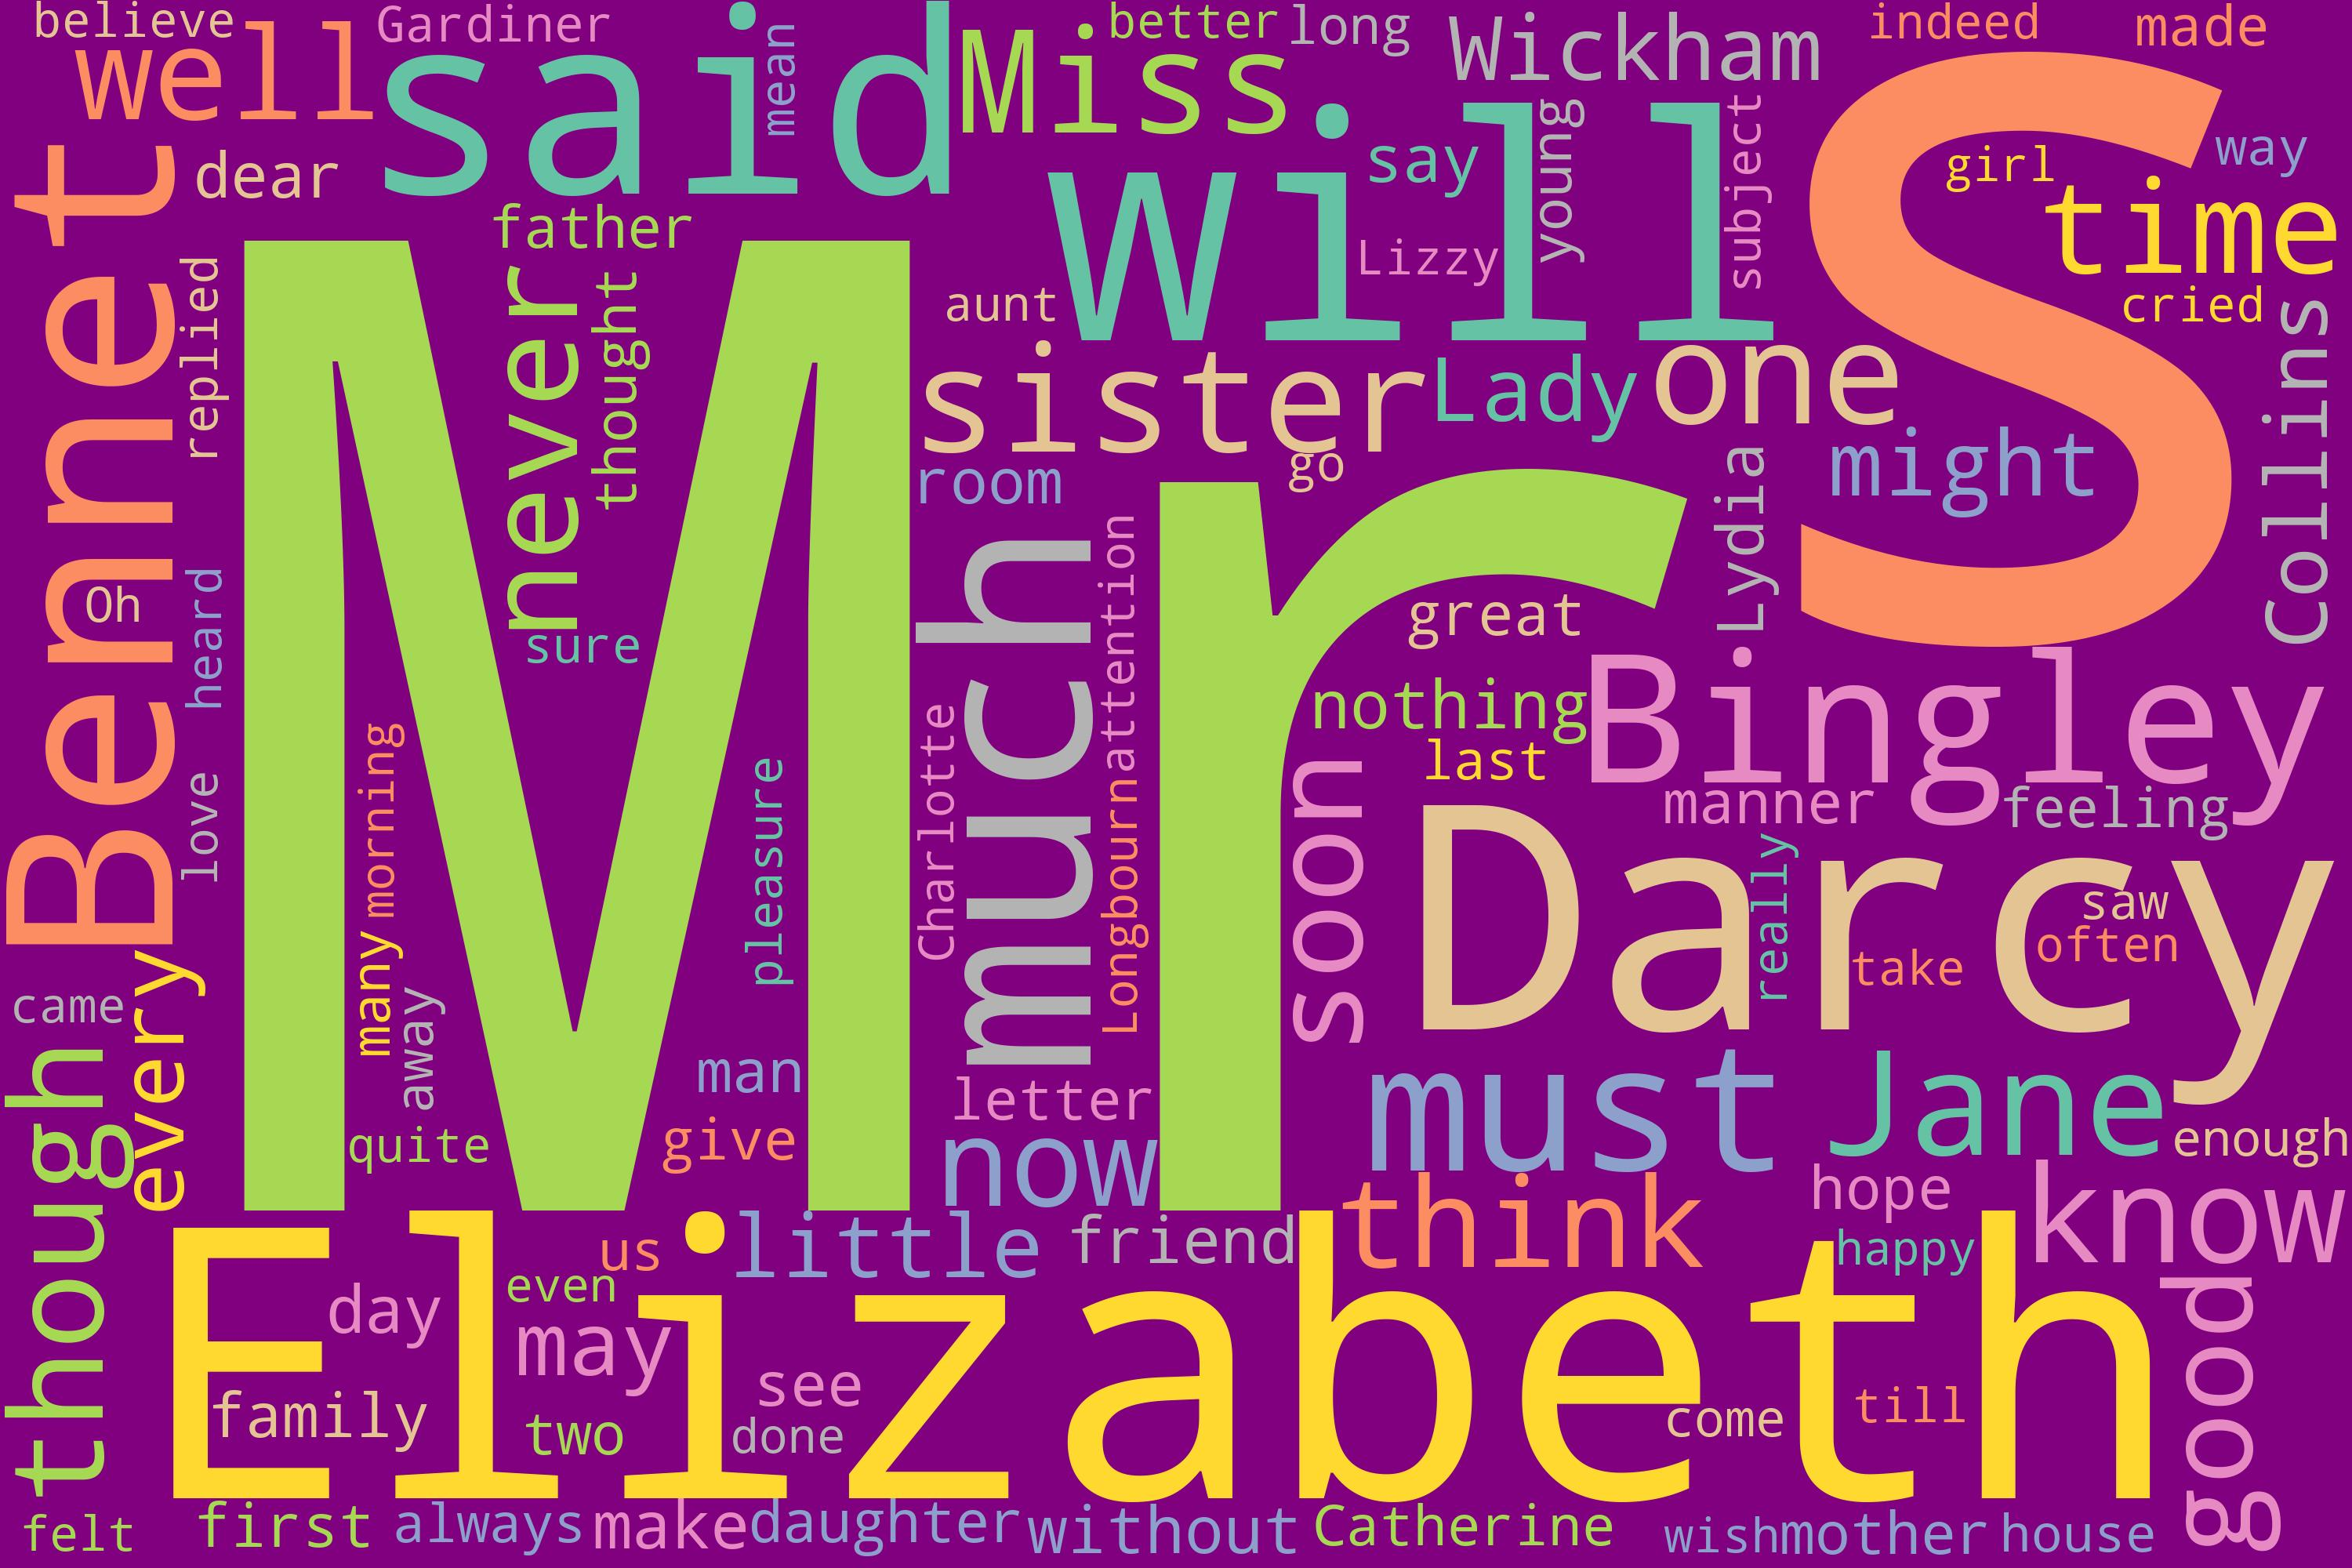
\includegraphics[width = 0.7\textwidth]{Images/PridePrejudice_JaneAusten.jpeg} % enter the filename here
		\caption{Word Cloud - Pride and Prejudice}
		\label{fig:pride-prejudice}
	\end{center}
\end{figure}

\begin{figure}[H]
	\begin{center}
		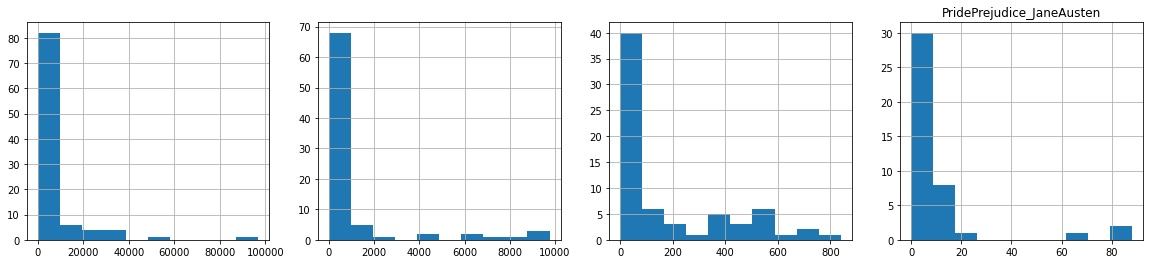
\includegraphics[width = 1.0\textwidth]{Images/char_hist_PridePrejudice_JaneAusten.jpeg} % enter the filename here
		\caption{Character Histogram - Pride and Prejudice}
		\label{fig:histogram-prideprejudice}
	\end{center}
\end{figure}



\subsection{\textcite{sherlock-holmes}} %enter the name of the subsection here
\label{sec:sherlock-holmes} % enter the subsection label here (for cross referencing)

The Adventures of Sherlock Holmes is a collection of twelve stories involving the famous London detective Sherlock Holmes and his associate Dr. Watson. The collection was published in October 1892, although the first Sherlock story appeared in the Strand Magazine in July 1891. In fact, the character of Sherlock Holmes first appeared in a short story called, A Study in Scarlet, published in Beeton's Christmas Annual in 1887. The themes of Sherlock Holmes are centered around four aspects, namely, Social Class, Justice, Deception, and Logic & Reason. \textcite{sherlock-holmes-summary}. Below is a quick word cloud from the complete book. 

\begin{figure}[H]
	\begin{center}
		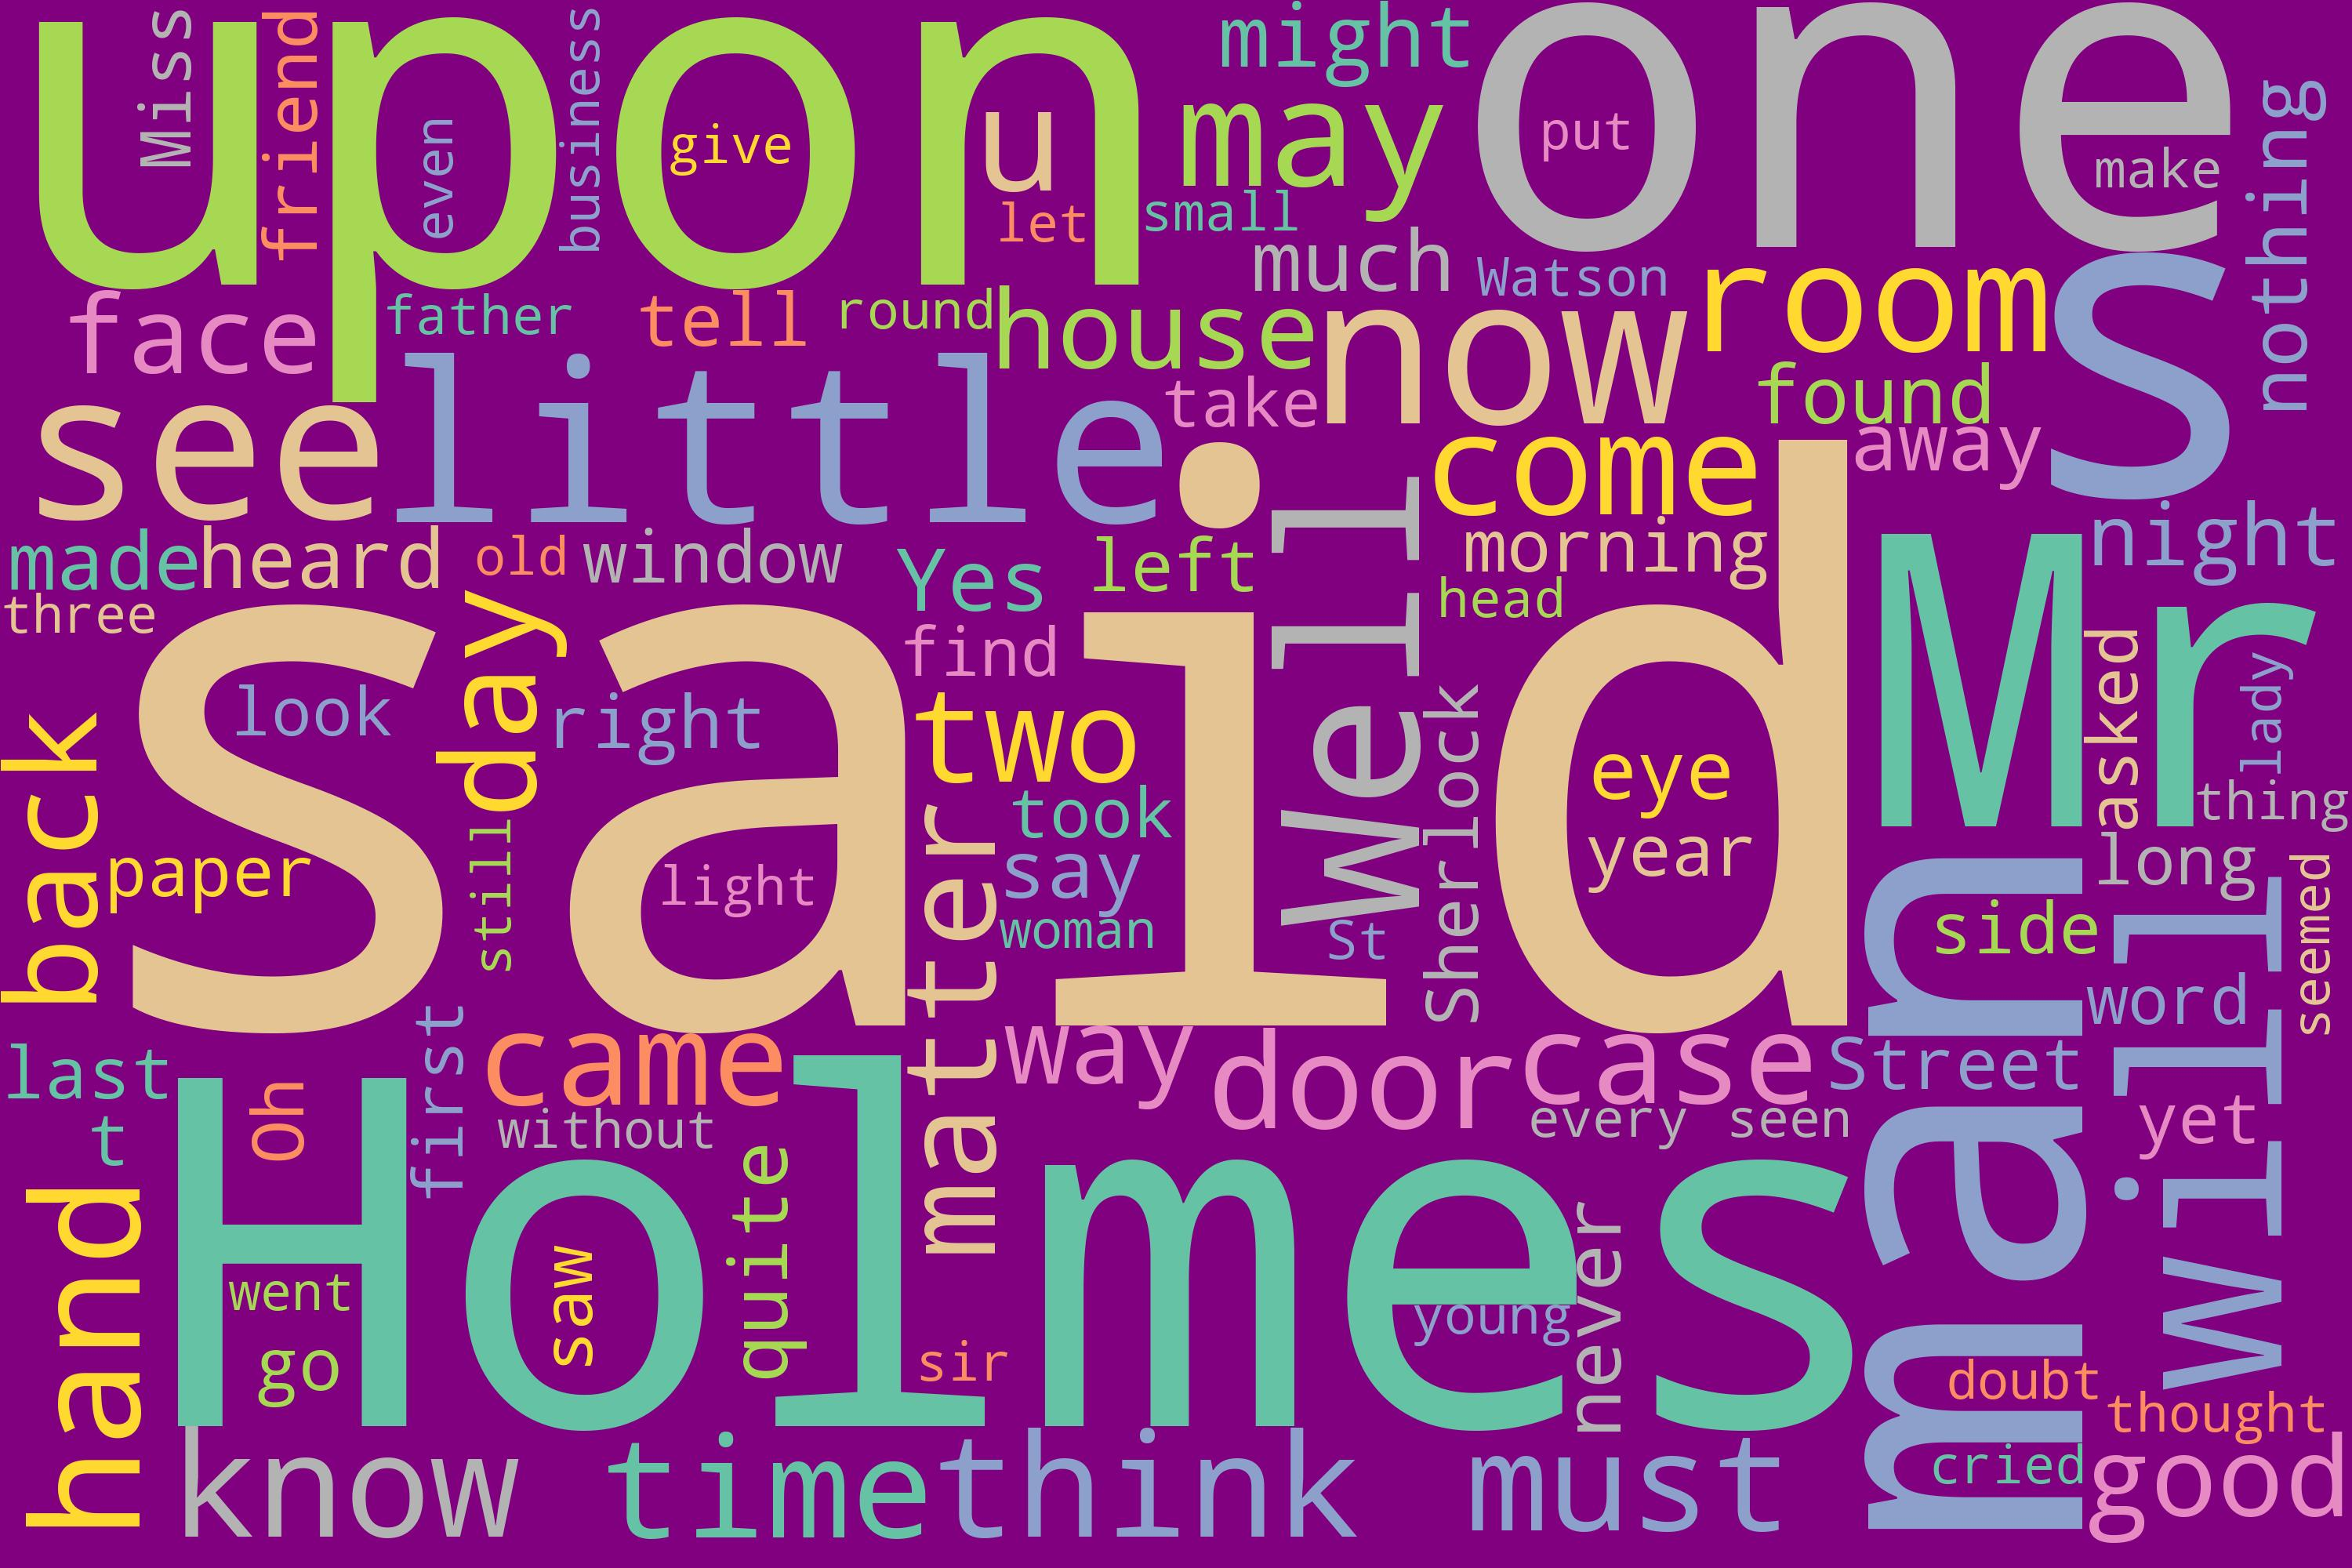
\includegraphics[width = 0.7\textwidth]{Images/SherlockHolmes_ArthurDoyle.jpeg} % enter the filename here
		\caption{Word Cloud - Sherlock Holmes}
		\label{fig:sherlock-holmes}
	\end{center}
\end{figure}

\begin{figure}[H]
	\begin{center}
		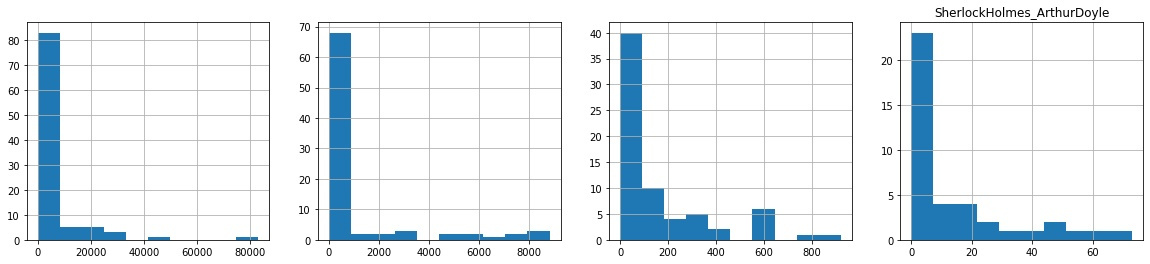
\includegraphics[width = 1.0\textwidth]{Images/char_hist_SherlockHolmes_ArthurDoyle.jpeg} % enter the filename here
		\caption{Character Histogram - Sherlock Holmes}
		\label{fig:histogram-sherlockholmes}
	\end{center}
\end{figure}

\subsection{\textcite{sign-of-the-four}} %enter the name of the subsection here
\label{sec:sign-of-the-four} % enter the subsection label here (for cross referencing)

The Sign of the Four is the second of Arthur Conan Doyle's Sherlock Holmes novels. In it, the detective and his companion Dr. Watson unravel a mystery of hidden treasure and murder. Miss Mary Morstan arrives at 221B, Baker Street to request help with the mystery of her missing father, her anonymous gifts of pearls, and a letter requesting her to meet an unknown person that evening. Holmes takes on her case and the adventure begins. Watson narrates the tale that sees the detective tracking down hidden treasure and murderers. By the end of the story the criminals are either dead or arrested, and Miss Mary Morstan and Watson are engaged to be married. \textcite{sign-of-the-four-summary}. Below is a quick word cloud from the complete book. 

\begin{figure}[H]
	\begin{center}
		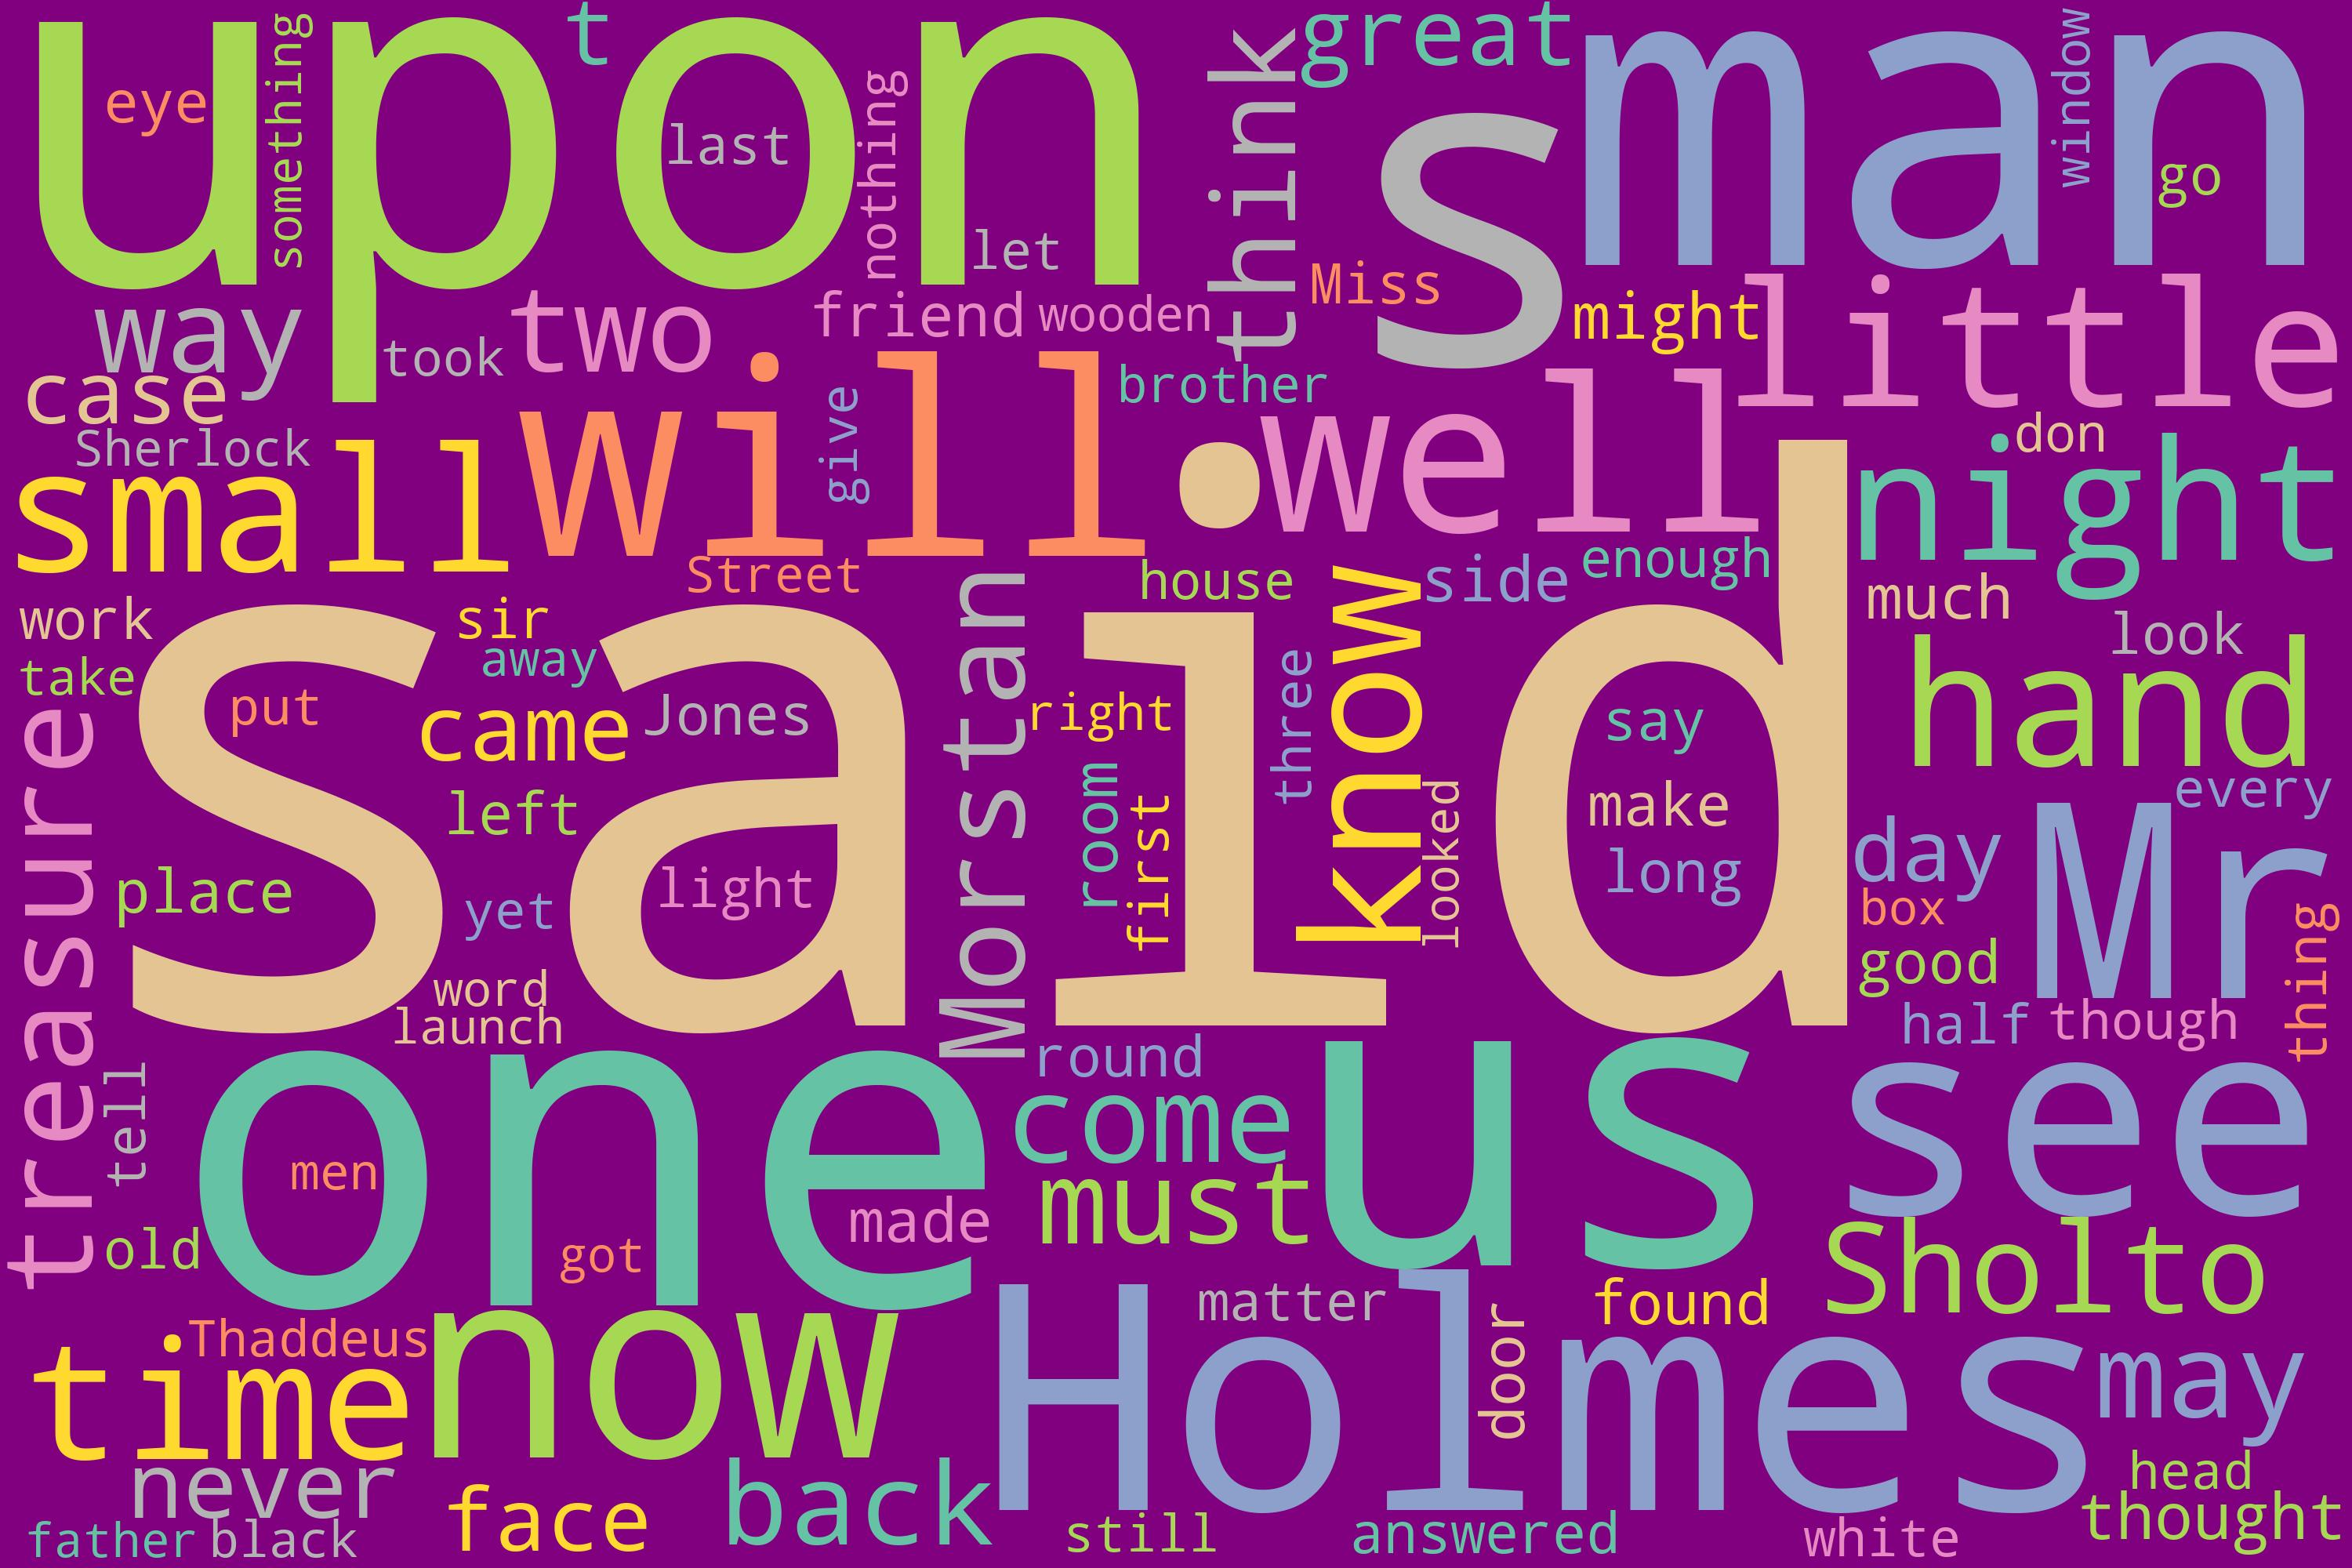
\includegraphics[width = 0.7\textwidth]{Images/SignOfTheFour_ArthurDoyle.jpeg} % enter the filename here
		\caption{Word Cloud - Sign of the Four}
		\label{fig:sign-of-the-four}
	\end{center}
\end{figure}

\begin{figure}[H]
	\begin{center}
		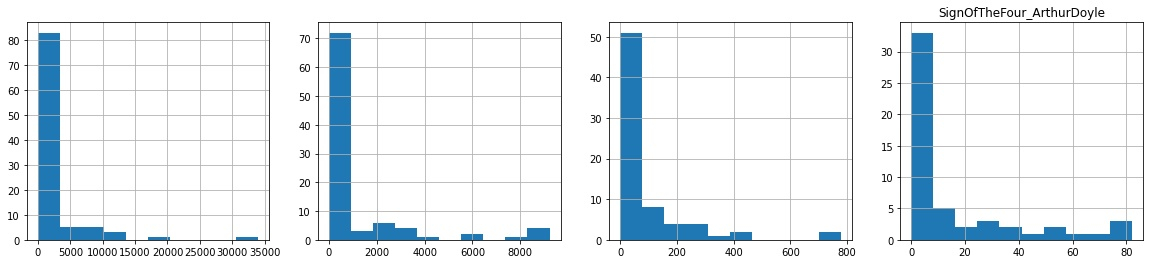
\includegraphics[width = 1.0\textwidth]{Images/char_hist_SignOfTheFour_ArthurDoyle.jpeg} % enter the filename here
		\caption{Character Histogram - Sign of the Four}
		\label{fig:histogram-signofthefour}
	\end{center}
\end{figure}

One key thing to notice is all of the histograms seem very skewed to the left. That's because a majority of the 98 characters do not actively occur in the entire text, mentioned in the section \ref{sec:unique-character-sets}. At maximum, we would see a corpus of 40 characters which would occur the most across all the text.

% ------------------------------------------------------------------------------
% Chapter 1
% Delete this content and replace it with your own
% ------------------------------------------------------------------------------
\chapter{Markov Chains} % enter the name of the chapter here
\label{cha:markov-chains} % enter the chapter label here (for cross-referencing)

In this section, we shall understand what Markov Chain does. But before we move with the main topic of our dissertation, let us understand why Markov Chains are as a concept and which problems they solve. Markov Chains is a stochastic statistical process, which derive usage from probabilities of occurrences of different events. Now these events can either be independent or dependent, and overall probabilities shall still be calculated based on the frequency within the provided data. Then that data can be used to perform additional classification work on a sample testing dataset.

However, a \textbf{stochastic process} is defined as follows:

\vspace*{\fill} 
\begin{quote}
\centering 
\textit{In probability theory and related fields, a stochastic or random process is a mathematical object usually defined as a family of random variables. Stochastic processes are widely used as mathematical models of systems and phenomena that appear to vary in a random manner.}
\end{quote}
\vspace*{\fill}

Next section, we shall go over the basic properties of a Markov Chain structure and its corresponding model.

\begin{itemize}
    \item The probabilities of moving from a state to all others sum to one, 
    \item The probabilities apply to all system participants, and 
    \item The probabilities are constant over time
\end{itemize}

\section{Markov Assumption} % enter the name of the section here
\label{sec:markov-assumption} % enter the section label here (for cross referencing)

In probability theory, Markov property refers to memory-less property of a stochastic process. The latter has the Markov property if the probability distribution of future states of the process conditioned on both the past and present states depends only on the present state. In other words, predicting the next word in a sentence depends only on the current word, and not on the words that came before the current word. Markov property holds in a model if the values in any state are influenced only by the values of the immediately preceding or a small number of immediately preceding states. The hidden Markov model (HMM) is an example in which it is assumed that the Markov property holds.

In general language, a model is an imitation of a real-world scenario.  Models allow us to try to understand and predict what might happen in the real world in a low-risk, cost-effective and fast way. For example, in order to predict how Amazon can ship its products in the most cost-effective ways, models are run in order to design routes and ensure minimal costs are incurred, thus optimizing these routes. 

An important distinction is between deterministic models and random models. Another word for a random model is a stochastic model. Deterministic models do not contain any random components, so the output is completely determined by the inputs and any parameters. Random models have variable outcomes to account for uncertainty and unpredictability, so they can be run many times to give a sense of the range of possible outcomes. 

\subsection{Stochastic Processes} %enter the name of the subsection here
\label{sec:stochastic-processes} % enter the subsection label here (for cross-referencing)

A stochastic process, which we will usually write as  $X_{n}$, is an indexed sequence of random variables that are usually dependent on each other. Now, $X_{n}$ consists of random variables which take a value within a \textbf{State Space} S. A state space can be either discrete or continuous and a discrete state space corresponds to a set of distinct outcomes which can be finite or infinite. A state space is nothing but a list of all possible values for a given event. Now the State Space S can be either discrete or continuous, depending on what the variable looks like. For our topic of the dissertation, we shall be focusing on novel textual data, thus our sample space or state space shall be characters ranging from $A-Z, a-z, 0-9$ or special characters. 

Furthermore, a stochastic process can be broken down into an Index Set, which brings in a time variable, providing some order to the entire process of indexing. This helps us make the entire process measurable over time. Thus, time can sometimes be selected as discrete intervals or continuous. A stochastic or 'random' process can be defined as four distinct processes based on \textbf{State Space} and \textbf{Index Set}.

\begin{itemize}
    \item \textbf{Discrete Time, Discrete Space} \\
    A major example of this shall be the number of students attending a maths lecture.
    \textbf{Markov Chains} is a perfect example of how discrete time and discrete space work in practice. Each node has a value, a weightage, and multiple yet finite edges based on a simple model.
    \item \textbf{Discrete Time, Continuous Space} \\
    Daily maximum temperature can be a good example of discrete time, which is one day, and continuous space, where the variables can take any value.
    \item \textbf{Continuous Time, Discrete Space} \\
    The number of visitors on a page over time, where total visitors vary over a defined number and time is continuous.
    \item \textbf{Continuous Time, Continuous Space} \\
    Levels of a share index, where values continue to fluctuate and generally do not remain in a defined discrete space of the shares of any company.
\end{itemize}

\begin{figure}[H]
	\begin{center}
		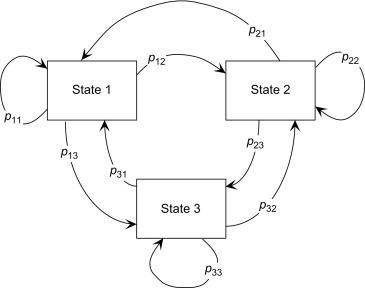
\includegraphics[width = 0.7\textwidth]{Images/markov_chain.jpg} % enter the filename here
		\caption{A simple example of states with discrete time.}
		\label{fig:markov-chain-state-space}
	\end{center}
\end{figure}

These Discrete Time Markov Chains are also what we shall be implementing in our novel classification problem further in the dissertation. We shall be focusing on a Discrete Space structure as part of the values. 

\section{Markov Property}
\label{sec:markov-property}
\textit{A stochastic process} $X = \left(X_{j}\right)_{j \in N_{0}}$ \textit{with values in a set space \textbf{S} is a Markov Chain if the following condition is met}.

\begin{equ}[!ht]
    \begin{equation}
    \begin{split}
        \label{eq:markov-chain-prop1}
        P \left( X_{j} \in A_{j} | X_{j-1} \in A_{j-1}, X_{j-2} \in A_{j-2}, \cdots, X_{0} \in A_{0} \right) \\ 
        &= P \left( X_{j} \in A_{j} | X_{j-1} \in A_{j-1} \right)
    \end{split}
    \end{equation}
\caption{\textit{$\forall A_0, A_1, \cdots, A_j \subseteq S$ and $j \in \mathbb{N}$}}
\end{equ}

This property works if the probability distribution $X_{j}$ depends on $X_{0}, \cdots, X_{j-2}$ through to $X_{j-1}$. And S is nothing but the state space or the sample space for the occurrence $\forall$ A. 

Now, let us try and demonstrate this property of Markov Chains through 2 simple examples.

\textbf{Example 1}: 
Let us denote $\left(\epsilon_{j}\right)_{j \in N_{0}}$ as identical independently distributed, i.e., i.i.d. random set of variables. The process X takes an assumption that $X_{0}$ = 0 and $X_j = X_{j-1} + \epsilon_j$, $\forall j \in \mathbb{N}$. If these conditions are satisfied, we can assume the model is a Markov Chain. And hence, we can denote $X_j$ as:
\begin{equ}[!ht]
    \begin{equation}
    \begin{split}
        \label{eq:markov-chain-prop1-ex1}
        X_j = \sum_{i = 1}^{j} \epsilon_{i}.
    \end{split}
    \end{equation}
\caption{In general, a Markov Chain is a random walk with some special cases.}
\end{equ}

\textbf{Example 2}: 
Let us denote $\left(\epsilon_{j}\right)_{j \in N_{0}}$ as identical independently distributed, i.e., i.i.d. random set of variables and this time, we have a variance of $Var\left(\epsilon_{j}\right)$ = 1. Then, this process can be given by $X_0$ = $X_1$ = 0 as the variance remains the same.

\begin{equ}[!ht]
    \begin{equation}
    \begin{split}
        \label{eq:markov-chain-prop1-ex2}
        X_{j} &= \frac{X_{j-1} + X_{j-2}}{2} + \epsilon_{j}
    \end{split}
    \end{equation}
\caption{And thus, $\forall$ j = 2,3,$\cdots$ is not a Markov Chain}.
\end{equ}

In the next two sections, we shall understand how the above Markov Property is useful when we distinguish between Discrete State Space Markov Chains and Continuous State Space Markov Chains.

\subsection{Discrete Space Markov Chains}
\label{sec:discrete-space-markov-chains}

In general working, when the state space is finite, such as for example, S = {1, 2, ..., N}, then the transition probabilities $P\left(X_{n} \in A_{n} | X_{n-1} \in A_{n-1}\right)$ in the equation \ref{eq:markov-chain-prop1} can be denoted with probabilities given by a short formula as 

\begin{equ}[!ht]
    \begin{equation}
    \begin{split}
        \label{eq:discrete-space-probdistro}
        p_{xy} = P \left( X_{j} = y | X_{j-1} = x \right)
    \end{split}
    \end{equation}
\caption{This equation is valid for all element pairs x, y $\in S$}.
\end{equ}

The resulting matrix P, which is derived by inserting values of the element pairs derived from the equation \ref{eq:discrete-space-probdistro}, i.e., $p_{xy}$ is known as the transition matrix. It would end up looking like this.

\begin{equ}[!ht]
    \begin{equation}
    \begin{split}
        \label{eq:discrete-time-transition-matrix}
        P = \left(
        \begin{array}{cccc}
        p_{11} & p_{12} & p_{13} & \cdots \\
        p_{21} & p_{22} & p_{23} & \cdots \\
        p_{31} & p_{32} & p_{33} & \cdots \\
        \vdots & \vdots & \vdots & \ddots
        \end{array}
        \right)
    \end{split}
    \end{equation}
\caption{This is how the transition matrix would be defined based on the number of variables we have}.
\end{equ}

When designing this transition probability matrix, we generally store a pair-mapping of each of the random variables and store their probability of occurrences. We shall see further that Markov Chains and Probability Matrices have a very deep relationship, as each distinct node can easily be considered a row and column value of this matrix. 
As an example, when we deal with characters as nodes in a Markov model, $p_{11}$ can be re-written as $p_{AA}$ if A is the first node of the model. It is pretty interchangeable but it can be simply explained as considering numerical numbers as an active denotation to simplify processes.

The matrix we considered is a finite one with limited variables. However, this transition matrix also works if we have an infinite state space and in those cases, our matrix P goes infinite as well. Now Discrete Markov Chains have a few Lemmas, which are important to keep in mind. Markov chains with finite or countably infinite state space are called Markov chains with \textit{discrete state space}.

\textbf{All of the following Lemmas are being taken from the book published by the Dr. Jochen Voss's taught module at the University of Leeds, and mentioned in their book, \textcite{voss:2013}}.

\subsubsection{Lemma 1}
\label{sec:discrete-markov-prop1}
Let $P^{SxS}$ be the transition matrix of a Markov Chain with state space, S. Then $P = \left(p_{xy}\right)_{x, y \in S}$ has the following properties:

\begin{enumerate}
    \item $p_{xy} \geq 0$ which stands true $\forall x, y \in S$.
    \item $\sum_{y \in S} p_{xy} = 1$ which stands true $\forall x \in S$. 
\end{enumerate}

A matrix that satisfies both the above conditions is known as a \textbf{stochastic matrix}. Additionally, a vector $\pi \in \mathbb{R}_{S}$ is called a probability vector, if $\pi_{x} \geq 0$ $\forall x \in S$ and $\sum_{x \in S} \pi_{x} = 1$. 

As we shall see in a later section, in order to simulate a Markov Chain, we shall require an input probability matrix $\pi$, and a transition matrix P, already defined to define any transition probabilities. For reference, the probability vector we shall be using is the probability of a novel occurring in a text and our probability of a character occurring in a novel would constitute the transition matrix.

\subsubsection{Lemma 2}
\label{sec:discrete-markov-prop2}

Let X be a time-homogeneous Markov chain with finite state space, and a transition matrix P. Then
\begin{equ}[!ht]
    \begin{equation}
    \begin{split}
        \label{eq:markov-discrete-lemma2}
        P \left( X_{j+k} = y | X_{j} = x \right) = \left( P^k \right)_{xy}
    \end{split}
    \end{equation}
\caption{$\forall j, k \in \mathbb{N}_{0}$ and $x, y \in S$, where $P^k = P. P \cdots P$ is the kth power of the transition matrix P}.
\end{equ}

Now we shall go about proving this lemma. That is important as need to figure out why time-homogeneous Markov chains function. 
\textbf{Proof}: For k = 0, the matrix $P^{0}$ is by definition the identity matrix and the statement
holds. Also, for k = 1 we have

\begin{equ}[!ht]
    \begin{equation}
    \begin{split}
        \label{eq:markov-discrete-lemma2-proof1}
        P \left( X_{j+1} = y | X_{j} = x \right) = p_{xy} = \left( P^1 \right)_{xy}
    \end{split}
    \end{equation}
\caption{by the definition of the transition matrix from equation \ref{eq:discrete-time-transition-matrix}}.
\end{equ}

Now we assume k $>$ 1 and the statement holds true for k-1, then we have

\begin{equ}[H]
    \begin{equation}
    \begin{split}
        \label{eq:markov-discrete-lemma2-proof2}
        P \left(X_{j+k} = y | X_{j} = x \right) \\
        &= \frac{P \left(X_{j+k} = y, X_{j} = x \right)}{P \left(X_{j} = x \right)} \\
        &= \frac{1}{P \left(X_{j} = x \right)} \sum_{z \in S} P \left(X_{j+k} = y, X_{j+k-1} = z, X_{j} = x \right) \\
        &= \frac{1}{P \left(X_{j} = x \right)} \sum_{z \in S} P \left(X_{j+k-1} = z, X_{j} = x \right) \\ &. P \left(X_{j+k} = y | X_{j+k-1} = z, X_{j} = x \right)  \\
    \end{split}
    \end{equation}
\caption{extended from the previous equation \ref{eq:markov-discrete-lemma2-proof1}}.
\end{equ}

Thus, using the Markov chain property from \ref{eq:markov-chain-prop1}, we use that property with this equation \ref{eq:markov-discrete-lemma2-proof2}

\begin{equ}[!ht]
    \begin{equation}
    \begin{split}
        \label{eq:markov-discrete-lemma2-proof3}
        P \left(X_{j+k} = y | X_{j} = x \right) \\
        &= \sum_{z \in S} \frac{P \left(X_{j+k-1} = z | X_{j} = x \right)}{P \left(X_{j} = x \right)} \\
        &= \sum_{z \in S} P \left(X_{j+k-1} = z | X_{j} = x \right) p_{xy} \\
        &= \sum_{z \in S} \left( P^{k-1} \right)_{xy} p_{xy}. 
    \end{split}
    \end{equation}
\caption{The above equation is basically a matrix-matrix multiplication of $P^{k-1}$ and $P$ probability transition matrices}.
\end{equ}

Now after we perform the matrix-matrix multiplication, we get the final equation of the Lemma 2.

\begin{equ}[!ht]
    \begin{equation}
    \begin{split}
        \label{eq:markov-discrete-lemma2-proof5}
        P \left(X_{j+k} = y | X_{j} = x \right) = \left( P^{k-1} . P\right)_{xy} = \left( P^{k} \right)_{xy}
    \end{split}
    \end{equation}
\caption{And we can summarize the lemma 2 using this equation above.}
\end{equ}


\subsubsection{Lemma 3}
\label{sec:discrete-markov-prop3}

Let X be a time-homogeneous Markov chain with finite state space and a transition state P and initial distribution $\pi$. Then we have 

\begin{equ}[!ht]
    \begin{equation}
    \begin{split}
        \label{eq:markov-discrete-lemma3}
        P \left(X_{j} = y\right) = \left(\pi^{T} P^{j}\right)_{y}
    \end{split}
    \end{equation}
\caption{$\forall y \in S$ }
\end{equ}

Now we shall go about proving this Lemma.

\textbf{Proof}: At time 0, the equation \ref{eq:markov-discrete-lemma3} can be reduced to

\begin{equ}[!ht]
    \begin{equation}
    \begin{split}
        \label{eq:markov-discrete-lemma3-proof1}
        P\left(X_{0} = x\right) = \pi_{x}
    \end{split}
    \end{equation}
\caption{$\forall x \in S$ }
\end{equ}

For time k $>$ 0, we can use Bayes' formula to come up with a summary as follows:

\begin{equ}[!ht]
    \begin{equation}
    \begin{split}
        \label{eq:markov-discrete-lemma3-proof2}
        P \left(X_{j} = y\right) = \sum_{x \in S} P \left(X_{j} = y | X_{0} = x\right) \\
        &= \sum_{x \in S} P \left(X_{0} = x\right) P \left(X_{j} = y | X_{0} = x\right) \\
        &= \sum_{x \in S} \pi_{x} \left( P^{j}\right)_{xy}
    \end{split}
    \end{equation}
\caption{$\forall y \in S$ }
\end{equ}

We need to consider a transposed vector $\pi^{T}$ as a matrix with one row and S columns, the equation \ref{eq:markov-discrete-lemma3-proof2} can be written as a matrix-matrix multiplication. 
Since X is a time-homogeneous Markov chain with a transition matrix, P. A probability matrix $\pi$ is called a \textit{stationary distribution} of X if $\pi^{T}.P = \pi^{T}$, leads us to the equation

\begin{equ}[!ht]
    \begin{equation}
    \begin{split}
        \label{eq:markov-discrete-lemma3-proof3}
        \sum_{x \in S} \pi_{x} p_{xy} = \pi_{y}
    \end{split}
    \end{equation}
\caption{$\forall y \in S$ }
\end{equ}

Now through the equation \ref{eq:markov-discrete-lemma3-proof1}, we already know that 

\begin{equ}[!ht]
    \begin{equation}
    \begin{split}
        \label{eq:markov-discrete-lemma3-proof4}
        P \left(X_{j} = y\right) = \left( \pi^{T} P^{j}\right)_{y}
    \end{split}
    \end{equation}
\caption{$\forall y \in S$ }
\end{equ}

\subsection{Continuous Space Markov Chains}

Even though we shall not be using continuous Markov chains for the purposes of our dissertation, we shall briefly understand what continuous Markov chains look like and go over their structure, how to incorporate them through an algorithm and take an example.

Markov chains can be considered on very general state spaces, but here we restrict ourselves to the case $S = \mathbb{R}^{d}$ . Most of the results from the previous section formally carry over to the case of continuous state space, with only changes in notation. Now instead of an infinite transition matrix P, we shall be using transition kernels which will be defined below.

A \textit{transition kernel} is a map $P\left(.,.\right)$ such that:

\begin{enumerate}
    \item $P \left(x, A\right) \geq 0$ for all $x \subseteq \mathbb{R}^{d}$ and all $A \subseteq {R}^{d}$; and 
    \item $P \left(x, .\right)$ is a probability distribution on $\mathbb{R}^{d}$ for all $x \in \mathbb{R}^{d}$.
\end{enumerate}

The idea behind a transition kernel is that it is a map of the distribution of the next value of the Markov chain. Keeping in mind that a continuous state space would tentatively have infinite values, a map would be the best idea to denote what the transition state could look like. Now, the map A $\rightarrow$ $P \left(x, A\right)$ is denoted as the distribution of the subsequent Markov chain. And hence, we can define the transition kernel with one equation below.

\begin{equ}[!ht]
    \begin{equation}
    \begin{split}
        \label{eq:markov-continuous-transition-kernel}
        P \left(x, A\right) = P \left(X_{j} \in A | X_{j-1} = x\right).
    \end{split}
    \end{equation}
\end{equ}

Additionally, there is a topic named transition density which comes into factor when dealing with continuous variables. Thus, if X is a Markov chain then the transition density is described as follows.

\begin{equ}[!ht]
    \begin{equation}
    \begin{split}
        \label{eq:markov-continuous-transition-density}
        P \left(X_{j} \in A | X_{j-1} = x\right) = \int_{A} p \left(x, y\right) dy
    \end{split}
    \end{equation}
    \caption{$\forall x \in \mathbb{R}^{d}$}
\end{equ}



\textbf{Algorithm of Markov chains with continuous state space} \\
Input: \\
A probability density π: Rd → [0,$\infty$) \\
A transition density p: Rd × Rd → [0,$\infty$) \\
Randomness used: \\
One sample $X_{0} \sim \pi$ \\
Samples from the densities $p \left(x, .\right)$ for $x \in \mathbb{R}$ \\
Output: \\
A path of a Markov chain with initial distribution $\pi$ and transition matrix P \\
1: Generate $X_{0} \sim \pi$ \\
2: Output $X_{0}$ \\
3: For $j = 1, 2, 3, \cdots $ \textbf{do} \\
4: Generate $X_{j} \sim$ $p \left( X_{j-1}, . \right)$ \\
5: Output $X_{j}$ \\
6: End for

This is the algorithm we would use to implement a continuous state Markov model. \\


\section{Markov Chain Example}

Now, we shall go over a sample example of a completely interconnected 3-state Markov Chain. When we solve for a Markov Chain, we try to solve for when all the states would return 1 as their final solution. 

\begin{figure}[htb]
\label{fig:markov-chain-example-1}
\centering
\begin{tikzpicture}
\node[state, align = center] (s1) {State 1};
\node[state, below right of=s1]  (s2) {State 2};
\node[state, below left of=s1] (s3) {State 3};

\draw (s1) edge[loop above] node {$1/4$} (s1);
\draw (s1) edge[bend left] node {$1/2$} (s2);
\draw (s1) edge[bend left=12] node {$1/4$} (s3);

\draw (s2) edge[bend left=12] node {$2/3$} (s1);
\draw (s2) edge[loop right] node {$1/6$} (s2);
\draw (s2) edge[bend right=12] node {$1/6$} (s3);

\draw (s3) edge[bend left] node {$1/6$} (s1);
\draw (s3) edge[bend right] node {$1/2$} (s2);
\draw (s3) edge[loop left] node {$1/3$} (s3);

\end{tikzpicture}
\caption{Example 1 of a 3-State Markov Chain}
\end{figure}

Therefore, the Transition Matrix of this completely interconnected Markov Model is denoted by:

\begin{equ}[!ht]
    \begin{equation}
    \begin{split}
        \label{eq:markov-chain-ex1}
        P = \left(
        \begin{array}{ccc}
        1/4 & 1/2 & 1/4 \\
        2/3 & 1/6 & 1/6 \\
        1/6 & 1/2 & 1/3
        \end{array}
        \right)
    \end{split}
    \end{equation}
\caption{Transition Matrix 1}.
\end{equ}

Similarly, if a few certain nodes end up missing, further is a second example:

\begin{figure}[htb]
\label{fig:markov-chain-example-2}
\centering
\begin{tikzpicture}
\node[state, align = center] (s1) {State 1};
\node[state, below right of=s1]  (s2) {State 2};
\node[state, below left of=s1] (s3) {State 3};

\draw (s1) edge[loop above] node {$3/4$} (s1);
\draw (s1) edge[bend left] node {$1/4$} (s2);
%\draw (s1) edge[bend left=12] node {$1/4$} (s3);

\draw (s2) edge[bend left=12] node {$2/3$} (s1);
%\draw (s2) edge[loop right] node {$1/6$} (s2);
\draw (s2) edge[bend right=12] node {$1/3$} (s3);

\draw (s3) edge[bend left] node {$1/6$} (s1);
\draw (s3) edge[bend right] node {$1/2$} (s2);
\draw (s3) edge[loop left] node {$1/3$} (s3);

\end{tikzpicture}
\caption{Example 2 of a 3-State Markov Chain}
\end{figure}

Therefore, the Transition Matrix of this completely interconnected Markov Model is denoted by:

\begin{equ}[!ht]
    \begin{equation}
    \begin{split}
        \label{eq:markov-chain-ex2}
        P = \left(
        \begin{array}{ccc}
        1/4 & 1/2 & 1/4 \\
        2/3 & 1/6 & 1/6 \\
        1/6 & 1/2 & 1/3
        \end{array}
        \right)
    \end{split}
    \end{equation}
\caption{Transition Matrix 2}.
\end{equ}
% Chapter 1
% Delete this content and replace it with your own
% ------------------------------------------------------------------------------
\chapter{Bayesian Classification} % enter the name of the chapter here
\label{cha:bayes} % enter the chapter label here (for cross-referencing)

Bayes Theorem provides a principled way for calculating a conditional probability.

It is a deceptively simple calculation, although it can be used to easily calculate the conditional probability of events where intuition often fails. Although it is a powerful tool in the field of probability, Bayes Theorem is also widely used in the field of machine learning. Its use in a probability framework for fitting a model to a training dataset and in developing models for classification predictive modeling problems such as the Bayes Optimal Classifier and Naive Bayes.

The main aim of this chapter is to provide some base for how Bayes' theorem works and how we could connect it with the main topic of our dissertation, Markov chains. Bayes' conditional probability has various uses and is even used in the probability matrix. And thus, at the end of this chapter, we shall understand four main knowledge pointers which are as follows:

\begin{itemize}
    \item Bayes Theorem definition and the methods involved in its implementation.
    \item Terms in the Bayes theorem calculation and their uses.
    \item Examples of Bayes theorem usage in classifiers, optimization, and causal models.
    \item Usage of Bayes' theorem in a discrete Markov chain model.
\end{itemize}

\section{Types of Probabilities} % enter the name of the section here
\label{sec:bayes-theorem-conditional-probability} % enter the section label here (for cross-referencing)

Before we understand what Bayes Theorem is, we need to be clear about what marginal, joint, and conditional probabilities are. 

In this section, we shall go over what they mean and how to implement them in theory. Probability is simply how likely something is to happen. Whenever we're unsure about the outcome of an event, we can talk about the probabilities of certain outcomes—how likely they are. Many events can't be predicted with total certainty. The best we can say is how likely they are to happen, using the idea of probability.

For example, the likeliness of a completely fair coin toss to yield Heads or Tails would exactly be 0.5 if the coin the absolutely balanced. This 0.5 is the probability of either Heads or Tails showing up at a given toss.

Now, let us go over what the different types of probabilities are.

\subsection{Marginal Probabilities} %enter the name of the subsection here
\label{sec:bayes-marginal-probabilities} % enter the subsection label here (for cross-referencing)

The probability of an event occurring $P \left(A\right)$, may be thought of as an unconditional probability.  It is not conditioned on another event. 
Marginal probability is the probability of an event, irrespective of other random variables. If the random variable is independent, then it is the probability of the event directly, otherwise, if the variable is dependent upon other variables, then the marginal probability is the probability of the event summed over all outcomes for the dependent variables, called the sum rule.

\textbf{Example 1}: The probability that a card drawn from a deck of 52 is red is given as $P\left(red\right) &= 0.5$. \\
\textbf{Example 2}: The probability that a card drawn from the same deck is a 4 is calculated to be $P\left(four\right) &= \frac{1}{13}$.

\subsection{Joint Probabilities}
\label{sec:bayes-joint-probabilities}

The joint probability is the probability of two (or more) simultaneous events, often described in terms of events A and B from two dependent random variables, e.g. X and Y. The joint probability is often summarized as just the outcomes, e.g. A and B is written as $P\left(A-and-B\right)$.  The probability of event A and event B occurring.  It is the probability of the intersection of two or more events.  The probability of the intersection of A and B may be written as $P \left( A \cap B \right)$.

\textbf{Example}: The probability that a card is a four and red shall be denoted and calculated as $P\left(four-and-red\right) &= \frac{2}{52} &= \frac{1}{26}$.  (There are two red fours in a deck of 52, the 4 of hearts and the 4 of diamonds).

\subsection{Conditional Probabilities}
\label{sec:bayes-conditional-probabilities}

The conditional probability is the probability of one event given the occurrence of another event, often described in terms of events A and B from two dependent random variables e.g. X and Y.
$P\left(A|B\right)$ is the probability of event A occurring, given that event B occurs. 

\textbf{Example}: Given that we drew a red card, what’s the probability that it’s a four $P\left(four|red\right) &= \frac{2}{26} &= \frac{1}{13}$. So out of the 26 red cards (given a red card), there are two fours that explain the calculation.

\section{Miscellaneous Probability Functions}

The joint probability can be calculated using conditional probability. The equation goes as follows:

\begin{equ}[!ht]
    \begin{equation}
    \begin{split}
        \label{eq:joint-prob-product-rule}
        P\left(A, B\right) &= P\left(A|B\right) * P\left(B\right)
    \end{split}
    \end{equation}
\caption{\textit{This is known as the product rule of probability}}
\end{equ}

Additionally, joint probability is symmetrical and thus, $P\left(A, B\right) = P\left(B, A\right)$.

Next, conditional probability is calculated using the joint probability, thus, we have the following equation.

\begin{equ}[!ht]
    \begin{equation}
    \begin{split}
        \label{eq:condn-prob-rule-p1}
        P\left(A | B\right) &= \frac{P\left(A, B\right)}{P\left(B\right)}
    \end{split}
    \end{equation}
\caption{\textit{Derivation of conditional probability through join probability}}
\end{equ}

However, conditional probability is not symmetrical. Thus, $P\left(A|B\right) \neq P\left(B|A\right)$.

Now, we can also calculate conditional probability through a secondary route. The next couple equations shall make that clearer.

\textbf{\begin{equ}[!ht]
    \begin{equation}
    \begin{split}
        \label{eq:condn-prob-rule-p2}
        P\left(A | B\right) &= \frac{P\left(B | A\right) * P\left( A\right)}{P\left(B\right)}
    \end{split}
    \end{equation}
\caption{\textit{This is the conditional probability formula}}
\end{equ}}

The reverse of this rule also works. Thus, 

\textbf{\begin{equ}[!ht]
    \begin{equation}
    \begin{split}
        \label{eq:condn-prob-rule-p2-rev}
        P\left(B | A\right) &= \frac{P\left(A | B\right) * P\left( B\right)}{P\left(A\right)}
    \end{split}
    \end{equation}
\caption{\textit{This is the conditional probability reverse formula}}
\end{equ}}

We use equations \ref{eq:condn-prob-rule-p2} and \ref{eq:condn-prob-rule-p2-rev} the most, as in most cases, joint probability from equation \ref{eq:joint-prob-product-rule} is tough to calculate in most cases. \textbf{These alternative equations of the conditional probabilities are known as Bayes' Rules or the Bayes' Theorem}.

\section{Bayes' Rule}
\label{sec:bayes-rule}

From equations \ref{eq:condn-prob-rule-p2} and \ref{eq:condn-prob-rule-p2-rev}, we were able to deduce that conditional probabilities do not need to rely on joint probabilities as the latter is a lot tougher to calculate and not generally available.

Thus, the final Bayes' Theorem can be deduced as follows.

\textbf{\begin{equ}[!ht]
    \begin{equation}
    \begin{split}
        \label{eq:bayes-rule-pb}
        P\left(B\right) &= P\left(B|A\right) * P\left(A\right) + P\left(B|not A\right) * P\left(not A\right)
    \end{split}
    \end{equation}
\caption{\textit{Conditional Probability designed around dependent event}}
\end{equ}}

Thus, we can use the equation \ref{eq:bayes-rule-pb} mentioned above in the conditional probability equation \ref{eq:condn-prob-rule-p2}, and have the rule re-defined as follows:

\textbf{\begin{equ}[!ht]
    \begin{equation}
    \begin{split}
        \label{eq:bayes-rule-pb-final}
         P\left(A | B\right) = \frac{\left(P\left(B | A\right) * P\left(A\right)\right)}{\left(P\left(B|A\right) * P\left(A\right) + P\left(B|not A\right) * P\left(not A\right)\right)}
    \end{split}
    \end{equation}
\caption{\textit{Conditional Probabilities}}
\end{equ}}

Additionally, keep in mind that $P\left(not A\right)$ is nothing but $1 - P\left(A\right)$. In the following sub-sections, we shall understand the terms of the Bayes' Rule.

\subsection{Terms of the Theorem}

The terms in the Bayes Theorem equation are given names depending on the context where the equation is used.

It can be helpful to think about the calculation from these different perspectives and help to map your problem onto the equation.

We need to keep in mind that the result $P\left(A | B\right)$ is referred to as the \textbf{posterior probability} and $P\left(A\right)$ is referred to as the \textbf{prior probability}. A quick link to an article explaining this is \textcite{ml_bayes_theorem}.

Similarly, $P\left(B | A\right)$ is referred to as the \textbf{likelihood} and $P\left(B\right)$ is referred to as the \textbf{evidence}.

\begin{itemize}
    \item $P\left(B | A\right)$ : Posterior Probability
    \item $P\left(A\right)$ : Prior Probability
    \item $P\left(B | A\right)$ : Likelihood
    \item $P\left(B\right)$ : Evidence
\end{itemize}

Let us explain the above terms with the help of an example. The example we shall take is exactly the topic of our dissertation. Let's say we need to find whether \textbf{novel A} is written by an \textbf{author A} or by \textbf{author B}, given we have another \textbf{novel B} written by one of these authors. We need to define the probability just on the basis of identifying all the texts from either of the books. Thus, let us consider $P\left(novel \textunderscore A\right)$ be the Prior, $P\left(novel\textunderscore A | author\textunderscore A\right)$ be the Likelihood and $P\left(author\textunderscore A\right)$ be the evidence.
Thus, this gives us the final equation:

\textbf{\begin{equ}[!ht]
    \begin{equation}
    \begin{split}
        \label{eq:bayes-rule-novel}
         P\left(author\textunderscore A | novel\textunderscore A\right) = P\left(novel\textunderscore A | author\textunderscore A\right) * P\left(author \textunderscore A\right) \div P\left(novel \textunderscore A\right)
    \end{split}
    \end{equation}
\caption{\textit{An example with novels}}
\end{equ}}

In the next couple section, we shall understand how Bayes' Formula can be used in Python as well as understand how Bayes' classifier can be built. 

\section{Code for Bayes' Rule}
\label{sec:python-bayes-rule}

Consider a human population that may or may not have cancer (Cancer is True or False) and a medical test that returns positive or negative for detecting cancer (Test is Positive or Negative). With this example, we shall be able to define the problem, as well as understand how to code Bayes' rule within Python. Now, with this scenario, we try to solve for the problem as follows :

\textit{If a randomly selected patient has the test and it comes back positive, what is the probability that the patient has cancer?}

We take this example from the article \textcite{ml_bayes_theorem}.

Medical tests are not free of errors. Thus, in order to predict whether a test which has given a positive result is truly positive or not, we consider a 2 by 2 matrix. This matrix is termed as the confusion matrix, which is used as a key metric in classification, which we shall delve deeper in the section \ref{sec:bayes-classification}.

\noindent
\renewcommand\arraystretch{1.5}
\setlength\tabcolsep{0pt}
\begin{tabular}{c >{\bfseries}r @{\hspace{0.7em}}c @{\hspace{0.4em}}c @{\hspace{0.7em}}l}
\label{Tab:confusion-matrix}
  \multirow{10}{*}{\parbox{1.7cm}{\bfseries\raggedleft actual}} & 
    & \multicolumn{2}{c}{\bfseries Confusion Matrix} & \\
  & & \bfseries p & \bfseries n & \bfseries total \\
  & p$'$ & \MyBox{True Positive}{} & \MyBox{False Negative}{} & P$'$ \\[2.4em]
  & n$'$ & \MyBox{False Positive}{} & \MyBox{True Negative}{} & N$'$ \\
  & total & P & N &
\end{tabular}

Before we begin with any coding, let us go over how to theoretically solve the table \ref{Tab:confusion-matrix}.

Sometimes a patient will have cancer, but the test will not detect it. This capability of the test to detect cancer is referred to as the sensitivity, or the \textbf{true positive} rate in the table \ref{Tab:confusion-matrix}. We will contrive a sensitivity value for the test. The test is good, but not great, with a true positive rate or sensitivity of 85 \%. That is, of all the people who have cancer and are tested, 85 \% of them will get a positive result from the test.

Therefore, $P\left(Test = Positive | Cancer = True\right) = 0.85$. 

Now similarly, we can use a contrived up number assuming the probability of cancer is low, and use a contrived base rate value of one person in 5,000, or (0.0002), 0.02 \%. Thus, $P\left( Cancer=True\right) = 0.0002$. There, using the equation \ref{eq:condn-prob-rule-p1}, we can redefine the equation for our needs as below.

\textbf{\begin{equ}[!ht]
    \begin{equation}
    \begin{split}
        \label{eq:bayes-rule-cancer}
        P\left( Cancer = True | Test = Positive\right) = \frac{P\left(Test=Positive | Cancer=True\right) * P\left(Cancer=True\right)}{P\left(Test=Positive\right)}
    \end{split}
    \end{equation}
\caption{\textit{Cancer example for Bayes' Rule}}
\end{equ}}

We know the probability of the test being positive given that the patient has cancer is 85\%, and we know the base rate or the prior probability of a given patient having cancer is 0.02\%. Similarly, from equation \ref{eq:bayes-rule-pb}, we get the following equation.

\textbf{\begin{equ}[!ht]
    \begin{equation}
    \begin{split}
    \begin{aligned}
        \label{eq:bayes-rule-cancer-2}
        P\left(Test=Positive\right) &= \\
        P\left(Test=Positive|Cancer=True\right) * P\left(Cancer=True\right) &+ \\
        P\left(Test=Positive|Cancer=False\right) * P\left(Cancer=False\right) \\
    \end{aligned}
    \end{split}
    \end{equation}
\caption{}
\end{equ}}

Now first, we calculate $P\left(Cancer=False\right)$ which is nothing but the inverse of cancer being true, which was 0.0002 in probability. Thus, $P\left(Cancer=False\right) = 1 - P\left(Cancer=True\right) = 1 - 0.0002 = 0.9998$. We still do not know the probability of a positive test result given no cancer. This requires additional information. Specifically, we need to know how good the test is at correctly identifying people that do not have cancer. That is, testing negative result (Test=Negative) when the patient does not have cancer (Cancer=False), called the true negative rate or the specificity. Let us use a random specificity for this value of 95 \%. Thus, $P\left(Test=Negative | Cancer=False\right) = 0.95$.  

Thus, with all this information, $P\left(Test=Positive|Cancer=False\right) &= \\  1 – P\left(Test=Negative | Cancer=False\right) = 1 - 0.95 = 0.05$. Thus, plugging in all the values into equation \ref{eq:bayes-rule-cancer-2}. $P\left(Test=Positive\right) = 0.85 * 0.0002 + 0.05 * 0.9998 = 0.05016$.

Excellent, so the probability of the test returning a positive result, regardless of whether the person has cancer or not is about 5 \%. Now, we finally have all the information needed to calculate the probability using our Bayes' Theorem and estimate whether a person has cancer or not based on whether or not they tested positive on a test. Inputting all the information into equation \ref{eq:bayes-rule-cancer}, we get the values as follows. 

$P\left(Cancer=True | Test=Positive\right) = \frac{0.85 * 0.0002}{0.05016} = 0.003389154704944$.

The calculation suggests that if the patient is informed they have cancer with this test, then there is only a 0.33\% chance that they have cancer. \textbf{This is a very bad diagnostic}. The test is completely unreliable. This is a little rare a case, and we typically have to calculate the bits we need and plug them in, as we did in this case. In our scenario, we were given 3 pieces of information, the base rate, the  sensitivity (or true positive rate), and the specificity (or true negative rate).

\begin{itemize}
    \item \textbf{Sensitivity:} 85\% of people with cancer will get a positive test result.
    \item \textbf{Base Rate:} 0.02\% of people have cancer.
    \item \textbf{Specificity:} 95\% of people without cancer will get a negative test result.
\end{itemize}

Now we finally show how we could code this in Python.

\begin{code}
\begin{minted}[frame=single,framesep=10pt]{python}
# Calculate P(A|B) given P(A), P(B|A), P(B|not A)
def bayes_theorem(p_a, p_b_given_a, p_b_given_not_a):
    # calculate P(not A)
    not_a = 1 - p_a
    # calculate P(B)
	p_b = p_b_given_a * p_a + p_b_given_not_a * not_a
	# calculate P(A|B)
	p_a_given_b = (p_b_given_a * p_a) / p_b
	return p_a_given_b

# P(A)
p_a = 0.0002
# P(B|A)
p_b_given_a = 0.85
# P(B|not A)
p_b_given_not_a = 0.05

# calculate P(A|B)
result = bayes_theorem(p_a, p_b_given_a, p_b_given_not_a)

# summarize
print('P(A|B) = %.3f%%' % (result * 100))
\end{minted}
\end{code}

This would end with the result printing as $P\left(A|B\right) = 0.339\%$.

Finally, in this section, we shall understand the ways a confusion matrix, mentioned in \ref{Tab:confusion-matrix} can be used to determine metrics for a classification system. There are three terms we shall be going in depth, and shall figure out the formula for each of them using the values from our confusion matrix. These terms are namely, \textbf{Precision, Recall and Accuracy}. Keep in mind, for the purposes of this task, we shall be referring to all the values via their abbreviation. Here are the terms we learnt about from the confusion matrix. 

\begin{itemize}
    \item True Positive : TP
    \item True Negative : TN
    \item False Positive : FP
    \item False Negative : FN
\end{itemize}

In all cases, the target of a confusion matrix and prior model development is to maximize the True Positives & False Negatives and minimize the True Negatives and False Positives. This leads us to the three terms mentioned above. Precision, Recall and Accuracy. These are simple formulae designed around the 2x2 confusion matrix, with which we can calculate the overall closeness within the model.
A true positive or true negative is a data point that the algorithm correctly classified as true or false, respectively. A false positive or false negative, on the other hand, is a data point that the algorithm incorrectly classified.

\subsection{Accuracy}
\label{sec:accuracy-confusion-matrix}

The exact formula for accuracy is as follows:

\textbf{\begin{equ}[H]
    \begin{equation}
    \begin{split}
    \begin{aligned}
        \label{eq:accuracy-confusion-matrix}
        Accuracy = \frac{TP + FN}{TP + TN + FP + FN}
    \end{aligned}
    \end{split}
    \end{equation}
\caption{}
\end{equ}}

\textbf{Accuracy} is the number of correctly predicted data points out of all the data points. More formally, it is defined as the number of true positives and true negatives divided by the number of true positives, true negatives, false positives, and false negatives. 

\subsection{Precision}
\label{sec:precision-confusion-matrix}

The exact formula for precision is as follows:

\textbf{\begin{equ}[H]
    \begin{equation}
    \begin{split}
    \begin{aligned}
        \label{eq:precision-confusion-matrix}
        Accuracy = \frac{TP}{TP + FP}
    \end{aligned}
    \end{split}
    \end{equation}
\caption{}
\end{equ}}

\textbf{Precision} is a useful metric in cases where False Positive is a higher concern than False Negatives. \textbf{Precision} is important in music or video recommendation systems, e-commerce websites, etc. Wrong results could lead to customer churn and be harmful to the business.


\subsection{Recall}
\label{sec:recall-confusion-matrix}

The exact formula for accuracy is as follows:

\textbf{\begin{equ}[H]
    \begin{equation}
    \begin{split}
    \begin{aligned}
        \label{eq:recall-confusion-matrix}
        Accuracy = \frac{TP}{TP + FN}
    \end{aligned}
    \end{split}
    \end{equation}
\caption{}
\end{equ}}

\textbf{Recall} is a useful metric in cases where False Negative trumps False Positive. \textbf{Recall} is important in medical cases where it does not matter whether we raise a false alarm but the actual positive cases should not go undetected.


\section{Bayes' Theorem for Classification}
\label{sec:bayes-classification}

Classification is a predictive modeling problem that involves assigning a label to a given input data sample. The problem of classification predictive modeling can be framed as calculating the conditional probability of a class label given a data sample. 

\textbf{\begin{equ}[H]
    \begin{equation}
    \begin{split}
    \begin{aligned}
        \label{eq:bayes-classification-p1}
        P\left(class|data\right) = \frac{P\left(data|class\right)}{P\left(data\right)}
    \end{aligned}
    \end{split}
    \end{equation}
\caption{Where $P\left(class|data\right)$ is the probability of a class given the some data.}
\end{equ}}

This calculation can be performed for each class in the problem and the class that is assigned the largest probability can be selected and assigned to the input data.

The priors for the class and the data are easy to estimate from a training dataset if the dataset is suitability representative of the broader problem. The conditional probability of the observation based on the class $P\left(data|class\right)$ is not feasible unless the number of examples is extraordinarily large, e.g. large enough to effectively estimate the probability distribution for all different possible combinations of values. This is almost never the case, we will not have sufficient coverage of the domain.


\subsection{Naive Bayes Classifier}
\label{sec:naive-bayes-classifier}

The main reason for using Bayes' Theorem for a conditional probability classification model is to ease the model of high-level calculations and overall, reduce the complexities involved. Bayes Theorem assumes that each input variable is dependent upon all other variables. This is a cause of complexity in the calculation. We can remove this assumption and go with the consideration that each of the input variables provided are random and independent of each other. In other words, the best way to consider a classification model with Bayes' Theorem would be to ensure all input variables are independently identically distributed (i.i.d.) over a given axis.

This changes the model from a dependent conditional probability model to an independent conditional probability model and dramatically simplifies the calculation. This means that we calculate $P\left(data|class\right)$ for each input variable separately and multiple the results together.
Thus, let us consider we have n variables, namely $x_1, x_2, x_3, \cdots, x_n$. We have one class defined over a given set of data. Then, we can use the equation \ref{eq:bayes-classification-p1} into a few smaller segments which remove the necessity of finding any combined probabilities. This gives us the following equation.

\textbf{\begin{equ}[H]
    \begin{equation}
    \begin{split}
    \begin{aligned}
        \label{eq:naive-bayes-classifier}
        P\left(class|x_1, x_2, \cdots, x_n \right) = P\left(x_1|class\right) * P\left(x_2|class\right) * \cdots * P\left(x_n|class\right) / P\left(data\right)
    \end{aligned}
    \end{split}
    \end{equation}
\caption{Where $P\left(class|data\right)$ is the probability of a class given the some data.}
\end{equ}}


\subsection{Bayes Optimal Classifier}
\label{sec:bayes-optimal-classifier}

The Bayes optimal classifier is a probabilistic model that makes the most likely prediction for a new example, given the training dataset. This model is also referred to as the Bayes optimal learner, the Bayes classifier, Bayes optimal decision boundary, or the Bayes optimal discriminant function.

Global optimization is a challenging problem of finding an input that results in the minimum or maximum cost of a given objective function. Typically, the form of the objective function is complex and intractable to analyze and is often non-convex, nonlinear, high dimension, noisy, and computationally expensive to evaluate.

Bayesian Optimization provides a principled technique based on Bayes Theorem to direct a search of a global optimization problem that is efficient and effective. It works by building a probabilistic model of the objective function, that is then searched efficiently with an acquisition function before candidate samples are chosen for evaluation on the real objective function.

Global Optimization is a major use of the Bayes Optimal Classifier, which works in tandem with an objective function. In the equation below, we share how Bayes Optimal Classifier works, but keep in mind, this is not a part of our dissertation topic. We are including this in order to have a wider and complete understanding of the Bayesian Classification subject. 

For the purpose of this equation, we figure out how to calculate the conditional probability for a new instance (vi) given the training data (D), given a space of hypotheses (H).

\textbf{\begin{equ}[H]
    \begin{equation}
    \begin{split}
    \begin{aligned}
        \label{eq:bayes-optimal-classifier}
        P\left(vj | D\right) = sum \{h in H\} P\left(vj | hi\right) * P\left(hi | D\right)
    \end{aligned}
    \end{split}
    \end{equation}
\caption{\textit{Where $vj$ is a new instance to be classified, $H$ is the set of hypotheses for classifying the instance, $hi$ is a given hypothesis, $P\left(vj | hi\right)$ is the posterior probability for $vi$ given hypothesis $hi$, and $P\left(hi | D\right)$ is the posterior probability of the hypothesis hi given the data $D$.}}
\end{equ}}

Now in the next and final theoretical chapter, we shall understand how we combine Markov Chains and Bayes' Theorem to predict which text is a part of which novel.



% ------------------------------------------------------------------------------
% Chapter 3

% ------------------------------------------------------------------------------

\chapter{Markov Chain Model for Text} % enter the name of the chapter here
\label{cha:markov_chain_text} % enter the chapter label here (for cross-referencing)

We shall now delve deeper into how Markov Chains can be effectively used with texts, and more specifically, Novels written by famous authors. Instead of traditional Markov Chains, we shall be using a combination of Bayes' Formula as well as Markov Chain probability distributions with a character level distinction. What we saw in the previous section is how Markov Chains connect different nodes, through edges with a certain weightage for each edge going from any Node A to Node B.

A short summary of how we shall perform Markov Chain Analysis with Novels is by creating a probability distribution transition matrix of all unique characters in each novel, using those probabilities as our edge weightage in Markov Chains, then finally train, test, and predict which text was written by a particular author.

\section{Character Tokenization} % enter the name of the section here
\label{sec:tokenization} % enter the section label here (for cross-referencing)

\textbf{Tokenization is essentially splitting a phrase, sentence, paragraph, or an entire text document into smaller units, such as individual words or terms}. In true essence, when working with large datasets, we tokenize all the text into small parts, for a type of batch processing. Since our process is restricted to working with unique characters, we shall be breaking words into smaller parts. Given a character sequence and a defined document unit, tokenization is the task of chopping it up into pieces, called tokens , perhaps at the same time throwing away certain characters, such as punctuation. \textcite{manning:2008}.

In NLP, textual data has been traditionally segmented into “sentences” (or “utterances”, etc.) and
“words” due to linguistic motivations and technical constraints. The macroscopic units (“sentences”) are often considered independently from one another and themselves segmented into microscopic units. The definition of these microscopic units has always been a matter of approximation and compromise. On the one hand, these units receive linguistic annotations (e.g. part-of-speech tags, morphosyntactic annotation, syntactic dependency information), which would require them to be linguistically motivated units. On the other hand, a large range of phenomena makes it highly non-trivial to identify and even consistently define linguistic units, denoted by the Morphological Annotation Framework (MAF) ISO standard as word forms. \textcite{DBLP:journals/corr/abs-2112-10508}.

Delving deeper, the main goal of Tokenization is building a vocabulary of any given text. This vocabulary is not only limited to words. It could be characters, phrases, or even sentences. Taking an example of speeches by different world leaders, the same message can be relayed by various leaders in completely different languages, dialects, or even the same language using synonyms, and holding unique styles in their speeches. Each separate and unique piece of text, character, word, or phrase is generally known as a \textbf{Token}. In general, when dealing with medium to large sets of texts, only 3 types of tokens are broadly used, which are classified as follows:

\begin{enumerate}
    \item \textbf{Characters}
    \item \textbf{Subwords} \textit{(A good example of sub-words would be happy, which is the root for multiple words, such as happiness, happily, happiest, happier, and happinesses. Thus, all these words would be considered a part of the root word in a tree word-mapping structure).}
    \item \textbf{Words} \textit{(In word tokenization, we are not working with word stemming or lemmatization. These processes fall under the subword tokenization structure and helps identify a complete vocabulary instead of small words or characters).}
\end{enumerate}

In terms of a quick visualization, here is how all three tokenization processes are implemented.

\begin{figure}[H]
	\begin{center}
		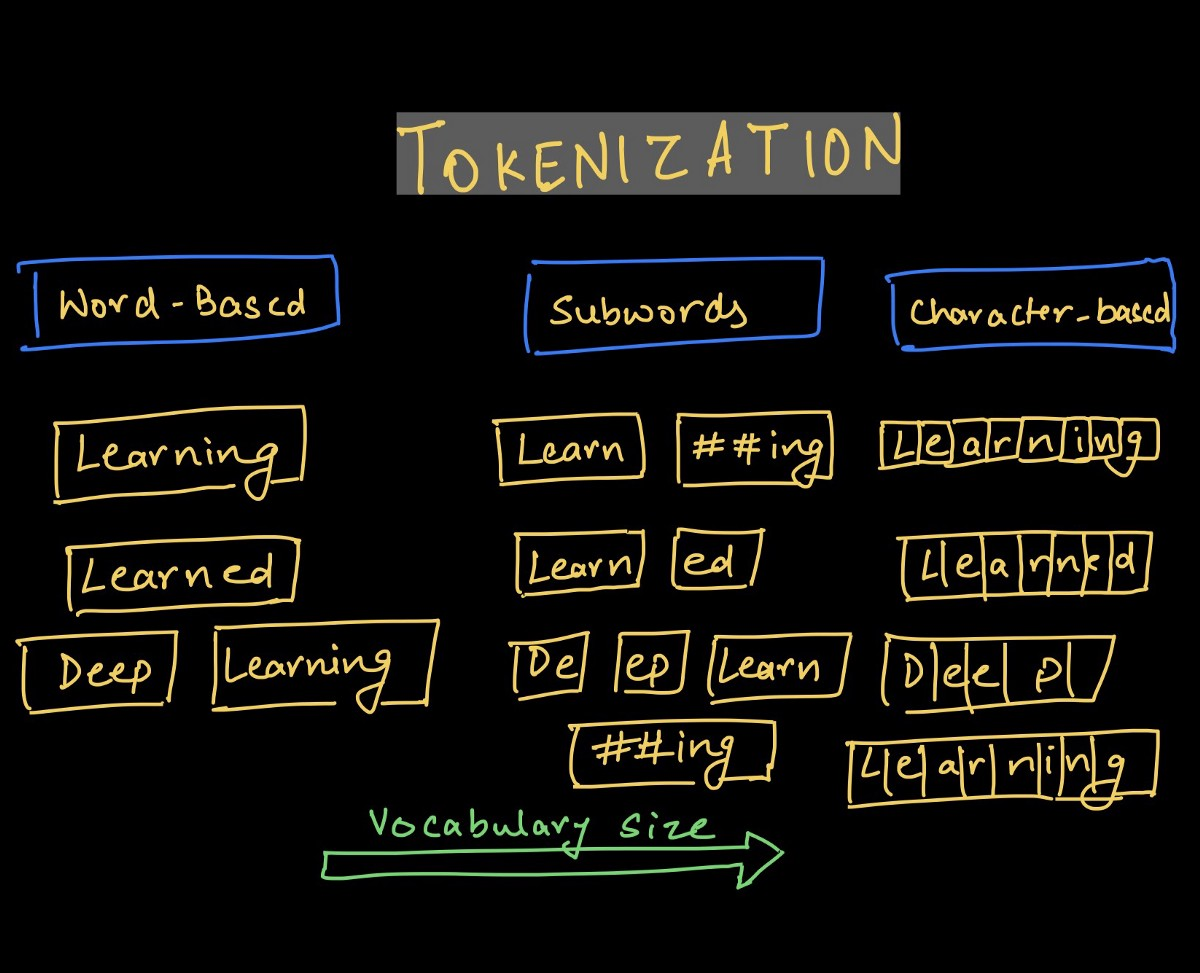
\includegraphics[width = 0.8\textwidth]{Images/tokenization.jpeg} % enter the filename here
		\caption{This is a quick example how character, subword and word tokenization works}
		\label{fig:tokenization-types}
	\end{center}
\end{figure}


If we deal with unique words or subwords, the number of tokens shall be much higher, leading to a much higher requirement of memory, space and computing power. In general working though, huge data models are trained on super-computers (as is the example of language translation of Google), then the model is released to the public, which constant upgrades and retraining taking place on the go.

Tokenization is the basic building block of any Natural Language Processing problem in machine learning. It is the most common process of solving any text prediction, one-hot embedding, or word-embedding problem, along with accessing raw text. 

One major problem also witnessed in Tokenization is the \textbf{OOV} (Out Of Vocabulary) issue. This causes the trained model to miss out on certain characters, words or subwords missed out during the training phase and are thus, encountered in the testing phase. This leads to the model not consisting of some tokens, causing errors in the prediction model. \textcite{tokenization_nlp_analyticsvidhya} .
However, these untrained tokens in words are generally solved by replacing the never-seen-before tokens with an \textit{$<$unknown token$>$} identifier. Since these words or characters are very rare in the main entire dataset, they are generally considered to have a very minuscule to nil effect on the final model. This would help in making sure the model is clean when tested, and does not create any out-of-memory error trying to retrain the same model upon revisitation.
 
\subsection{Character Tokenization} %enter the name of the subsection here
\label{sec:token_characters} % enter the subsection label here (for cross-referencing)

Characters are not limited to just English letters. It could be special characters like brackets({}, (), []), colons or semi-colons, numbers, etc. This breaks down the complete dataset into its most fundamental elements, creating a character-wise probability distribution that acts as the character weightage for our Markov Chain edges and nodes.

As discussed in previous sections and what shall be seen in the next sections we shall be utilizing character tokens are part of this project. The reason for this being we wish to delve deeper into how different novelists and authors use unique characters in their books. A detailed analysis of this shall be available in later sections as well. 

This trick in NLP can be considered quite useful when dealing with a smaller memory for the training model, and the size of the dataset would have a much lesser requirement of RAM or GPU for data processing. This is because characters, which can include letters from different languages, special characters such as semi-colons or commas, and numerical characters can be limited to maybe a maximum of a couple of hundred unique tokens.
Now, while this technique is much lower computationally expensive, character tokenization has a few drawbacks on its own.

\begin{itemize}
    \item Character tokens solve the OOV problem but the length of the input and output sentences increases rapidly as we are representing a sentence as a sequence of characters. As a result, it becomes challenging to learn the relationship between the characters to form meaningful words.
    \item If a single character is missed out from the training dataset, the actual relationship of the character with other tokens would be completely lost as the previously-not-seen character would be considered an \textit{$<$unknown token$>$}.
\end{itemize}

\subsection{Subword Tokenization}
\label{sec:token_subwords}

The core concept behind subwords is that frequently occurring words should be in the vocabulary, whereas rare words should be split into frequent subwords. Eg. The word “refactoring” can be split into “re”, “factor”, and “ing”. Subwords “re”, “factor” and “ing” occur more frequently than the word refactoring, and its overall meaning is also kept intact. \textcite{subwords_tokenization}. 

Since a majority of this project is focused on character tokenization and not subwords, we shall briefly understand all the different types of active subword tokenizations.

For reference to how subwords are broadly used, these are some of the most widely used techniques.

\begin{itemize}
    \item \textbf{Byte-Pair Encoding}, i.e., BPE was introduced in the article, \textcite{DBLP:journals/corr/SennrichHB15}, which explains how we can use Neural Machine Translations and extract all the words into an occurrence-based encoding, leading to either a word-wise or character-wise byte-pairing. Byte Pairing, however, has a distinction between train and test datasets, and would end up including some $<$unknown tokens$>$ in the test set.
    \item \textbf{WordPiece Tokenization}, works similar to Byte-Pair Encoding, with the exception that all the characters or words are already included in the vocabulary. This completely eradicates the need for unknown token generation and maximizes the likelihood of the training data and minimizes any training loss.
    \item \textbf{SentencePiece Tokenization}, does not treat space as a separator, instead, it takes the string as input in its original raw format, i.e. along with all spaces. It then uses BPE or unigram as its tokenizers to construct the vocabulary. In this case, words are pre-tokenized with a special character, which could be \textunderscore , or -, or any other distinctive character token.
\end{itemize}

\subsection{Word Tokenization}
\label{sec:token_words}

Word Tokenization, is among the most widely used algorithm in NLP, as it stores the essense of words in sentences while a model is trained. During word tokenization, there is no change in the final words, rather, stop words are removed, word-stemming and lemmatization takes place and root-words are separated from the actual text. A number of techniques, such as GloVe, Word2Vec, are used for the vectorization of words into word embeddings for a graphical representation, based on the overall probability of occurance in pre-trained or newly trained NLP models.

When dealing with words, there are a number of issues one can face. Some of them are as follows:

\begin{itemize}
    \item \textbf{OOV Words}, also stated above as \textbf{Out-Of-Vocabulary} words, certain words tend to be rare in the dataset. In order to handle these missing words, only the Top-K Frequent words are included in the dictionary and the remaining missing words are handled as \textit{$<$unknown token$>$}.
    \item \textbf{$<$unknown token$>$}, are missing words, which have been replaced in the vocabulary, and are very rare. However, the word mapping is lost in case of UNK tokens.
    \item \textbf{Large Vocabulary}. In this issue, most of the models we see today have been trained over huge corpus of text, which could range from twitter to novels to article datasets. In order to improve any of the models, a large amount of memory would be needed to train these models all over again.
\end{itemize}

Due to these drawbacks, we also sometimes focus on character tokenization of small datasets, which would preserve the overall structure of words, but ends up missing out on sentence formation and containing the meaning of words.


% ------------------------------------------------------------------------------
% Referencing examples
% ------------------------------------------------------------------------------
\section{Custom Bayes' Rule Implementation}
\label{sec:custom-bayes-implementation}

From what we learnt in the previous chapter, Naive Bayes' formula is very useful calculating underlying probabilities of 'A' given 'B'. 

Since we are using character tokens for our novels, we work with a custom Bayes' formula. Before we go on to the custom formula, let us consider an example.

\begin{equ}[!ht]
  \begin{equation}
    \label{eq:bayes-2}
    P(\theta|\textbf{D}) = \frac{P(\theta ) * P(\textbf{D} |\theta)}{P(\textbf{D})} ~~~~~|| I,
  \end{equation}
\caption{where {\texttheta} is the target and \textbf{D} is the feature}
\end{equ}

While in a normal Naive Bayes' theorem we have one target and one feature, we work with a custom form while working over our character tokenization problem, creating a probability matrix for each novel we work with. However, with a customized Bayes' Theorem, we work with multiple features. Let us consider an example for the same.

\begin{equ}[!ht]
  \begin{equation}
    \label{eq:characters_all}
    x_{1}, x_{2}, ..., x_{n} \in \textbf{A}
  \end{equation}
\caption{where $x_{k}$ are all the distinct characters and \textbf{A} are all real characters.}
\end{equ}

In general, when dealing with a specific language, the vocabulary is restricted to the characters found within that language. For example, with English, we are dealing with a vocabulary of about 94 characters, which includes special characters, numerals, capital and small letters. An extended example is provided in the image \ref{fig:english-characters}. With it, we can understand how each character would have a different weightage, once we have a broader understanding of the complete vocabulary for our custom Bayes' Rule.

\begin{figure}[H]
	\begin{center}
		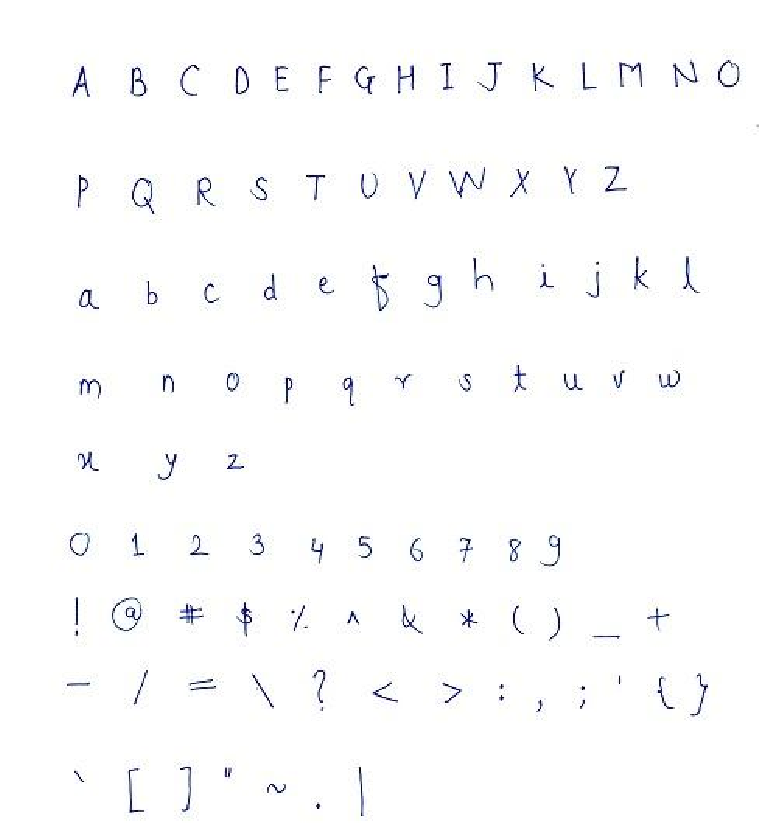
\includegraphics[width = 0.7\textwidth]{Images/english_characters.png} % enter the filename here
		\caption{An exhaustive list of all English characters \cite{english_characters}.}
		\label{fig:english-characters}
	\end{center}
\end{figure}

Keeping in mind the true formula of Bayes' Rule from the equation \ref{eq:bayes-2}, our target \texttheta is the variable for our novel we are trying to predict, and \textbf{D} is/are the features we have, i.e, our character sets. For each target, the overall characters shall remain the same as the number of characters does not budge. Thus, our features remain static and the prediction algorithm works over the probabilities. 

Bayes' Formula, which works over probabilities on the occurrences, determines the extent to which an event is supposed to occur. However, the summation of all the probabilities of an event always sums up to 1.


\begin{equ}[!ht]
    \begin{equation}
        \label{eq:probabilities_sum}
        \sum_{a \in \textbf{A}} P_x^{\left ( i \right )} = 1
    \end{equation}
\caption{$\forall$ events 'i' and features 'x'}
\end{equ}

Now with this equation, we move ahead with an assumption that all probabilities sum up to 1 for each event in the matrix. After this, we shall be able to move ahead with the overall structure of our Custom Naive Bayes' theorem, which can be a good predictor of the occurrence of randomized conditions. With this assumption, let us consider our custom Bayes' formula.

\newline

\begin{equ}[!ht]
    \begin{equation}
        \label{eq:custom_bayes_p1}
        P \left ( i | x_{1}, x_{2}, \cdots, x_{n} \right ) &= \frac{P \left (x_{1}, x_{2}, \cdots, x_{n} | i \right ) . \pi \left ( i \right )}{P \left (x_{1}, x_{2}, \cdots, x_{n} \right )}
    \end{equation}
\caption{$\forall$ events 'i' and features 'x', a custom Bayes' Theorem}.
\end{equ}

In the equation \ref{eq:custom_bayes_p1}, we mainly deal with probabilities. 
\begin{itemize}
    \item $\pi \left ( i \right )$ is the probability of an event 'i' occurring.
    \item $P \left ( i | x_{1}, x_{2}, \cdots, x_{n} \right )$ is the probability of event 'i' occurring given $x_{1}, x_{2}, \cdots, x_{n}$ occur.
    \item $P \left (x_{1}, x_{2}, \cdots, x_{n} | i \right )$ is the probability of $x_{1}, x_{2}, \cdots, x_{n}$ occurring given that event 'i' has already transpired.
\end{itemize}


Now, the denominator $P \left (x_{1}, x_{2}, \cdots, x_{n} \right )$, is just the probabilities of our features 'x' occurring over a given event. This means, however small the product of the probabilities be, they shall remain constant for the event 'i'. Similarly, $\pi_{i}$ is the probability of an event 'i' occurring and for all events, the probability shall remain constant. 

Thus, moving ahead, we can replace the equality with a proportionality instead since we have two variables that remain constant for an event 'i'. Thus, our new custom Bayes's Rule can be summarised as follows.

\begin{equ}[!ht]
    \begin{equation}
        \label{eq:custom_bayes_p2}
        P \left ( i | x_{1}, x_{2}, \cdots, x_{n} \right ) &\propto \Pi_{j = 1}^n P_{x_j}^{\left ( i \right )} . \pi \left ( i \right )
    \end{equation}
\caption{\textit{The R.H.S. is a product of all of the feature probabilities}}.
\end{equ}

Considering we would have to deal with values of the feature probabilities all ranging from [0, 1], the best option would be to take a log of the probabilities of $x_1, x_2, \cdots, x_n$ combined, and according to the product rule of log, we would just need to sum up the log probabilities individually. In terms of an equation, we state it at follows.

\begin{equ}[H]
    \begin{equation}
    \begin{split}
        \label{eq:custom_bayes_p3}
        \log_e \left ( P \left (x_{1}, x_{2}, \cdots, x_{n} | i \right ) \right ) &= \log_e \left ( \Pi_{j = 1}^n P_{x_j}^{\left ( i \right )} . \pi \left ( i \right ) \right ) \\
        &= \sum_{j = 1}^n \log_e P_{x_j}^{\left ( i \right )} + \text{Const.} \\
        &= \sum_{j = 1}^n \log_e P_{x_j}^{\left ( i \right )} - \max_{j} \log_e P_{x_j}^{\left ( k \right )}
    \end{split}
    \end{equation}
\caption{\textit{Log of a product leads to the summation over individual Logs}}
\end{equ}

A short summary of equation \ref{eq:custom_bayes_p3}, we obtain a $\textbf{Const.}$ upon taking the logarithm over $\pi \left ( i \right )$, we take the $\max_{j} \log_e P_{x_j}^{\left ( k \right )}$ as the constant because \textbf{each iteration would add an additional maximum value of and each event would have a new adjustment factor}. \textit{Please note, the maximum we take is over all the novels we are working alongside and not just a single character maximum}.

Now each of our Bayes' rule probabilities are stored as effective weights for our Markov Chain model's edges and useful for connecting nodes. We add the constant at the end of equation \ref{eq:custom_bayes_p3} so as to adjust for any bias. One key change we have made is adding a $\log_e$ to the custom rule. Thus, in order for this logic to function, we would need to take an exponent to revert back to the actual probability.

Finally, we can concise all the equations above in the next final equation, which becomes the basis of our complete project, \textbf{which is to predict which piece of text was authored by which novelist}. 

\begin{equ}[H]
    \begin{equation}
    \begin{split}
        \label{eq:final_custom_bayes}
        \log_e \left ( P \left (L | X_{1} = W, X_{2} = E \right ) \right ) &= \log_e \left ( P \left (X_{1} = W, X_{2} = E | L \right ) . P \left ( L \right ) \right ) \\
        &= \log_e ( P \left (X_{1} = W, X_{2} = E | L \right ) + \left(n . \log_e P \left ( L \right ) \right ) \pm  \log_e \left( Const. \right)
    \end{split}
    \end{equation}
\caption{\textit{Summarization of the custom formula for Bayes' Rule and Markov Chains}}
\end{equ}

There are multiple reasons why a log was the best solution. We shall state them as follows:

\begin{enumerate}
    \item Probabilities are always between [0, 1) and upon multiplying small numbers, ex: 0.01 * 0.001 = 0.00001, which would yield computationally insignificant results.
    \item With Logarithms at this step, we eliminate the possibility of a variable's impact in the final model going zero. Instead, that log converts the probability into a negative number for further calculations.
    \item Each event would have its own probability, and with negative logs, prediction over the test set shall be much easier.
\end{enumerate}

\section{Custom Bayes' Rule Example}
\label{sec:custom-bayes-example}

In this section, we shall see a quick example of how we would train a text dataset based on its probabilities and use Bayes' Rule to solve that issue. As we have seen in \ref{sec:custom-bayes-implementation}, each and every value needs to be given equal importance. Thus, we take a log of the values as lower values would end up being considered negligible by a simple model, and thus, result in data loss.

Let us show this as an example. 

Say we have two pieces of text and let's call them events. 
$ABCB$ and $BACCA$. Now, since we already know the length of the strings, and all the unique characters are present, we can easily compute their respective character probabilities. Let $ABCB$ be event 1 and $BACCA$ be event 2 for the purposes of our example.

\begin{equ}[H]
    \begin{equation}
    \begin{split}
        \label{eq:custom_train_example}
        Event_1 \\
        P\left(A\right)^{\left(1\right)} = 1/4 \\
        P\left(B\right)^{\left(1\right)} = 1/2 \\
        P\left(C\right)^{\left(1\right)} = 1/4 \\
        --------\\
        Event_2 \\
        P\left(A\right)^{\left(2\right)} = 2/5 \\
        P\left(B\right)^{\left(2\right)} = 1/5 \\
        P\left(C\right)^{\left(2\right)} = 2/5 \\
    \end{split}
    \end{equation}
\caption{\textit{Example of the Bayes' Rule above}}
\end{equ}

Consider the training examples we have. \textbf{ABCB} and \textbf{BACCA}, which we shall use in order to present generate an extremely elementary Markov Chain model. With this, we separate each text into its elemental units, i.e., characters. And then we calculate the probabilities of each character within each piece of text. Thus, ensuring the total probabilities sum up to 1. Now, we shall test a simple piece of text and then use it to possibly predict which sequence of characters works best with it.

Thus, we can next, calculate the probabilities from the information we calculated in equation \ref{eq:custom_train_example}. Let us consider we have a new piece of text, $BBC$, for which we need to predict which event did this test tentatively originate from.


\begin{equ}[H]
    \begin{equation}
    \begin{split}
        \label{eq:custom_test_example}
        Test \\
        P\left(BBC | event_1\right) = 1/2 * 1/2 * 1/4 = 1/16 = 0.0625 \\
        P\left(BBC | event_1\right) = 1/5 * 1/5 * 2/5 = 2/125 = 0.016 \\
        --------\\
        Now, 0.0625 > 0.016
    \end{split}
    \end{equation}
\caption{\textit{Example of the Bayes' Rule above}}
\end{equ}

From both these examples above, we can quickly see that $P \left ( 'BBC' | event_{1} \right )$ gives an yield of 0.0625 probability whereas the $P \left ( 'BBC' | event_{2} \right )$ shows us this probability of occurrence goes down to 0.016. Thus, we can consider that 'BBC' could be predicted as being a part of event 1 rather than event 2 in our machine learning model.

Since our target was to use character-level Markov Chains, and the key characteristic of any Markov Chain model is that each weight going out of a node sums up to one, we perform this over a complete novel, in order to better capture the results of how prediction could work for a particular piece of text when dealing with a number of different authors. In order to predict the final outcome in predicting the right novel, we shall create a transition matrix, which is depicted as a probability matrix for each novel corresponding to each character. 

\section{Laplacian Smoothing}
\label{sec:laplace-smoothing}

In general, Laplace Smoothing is also termed as Additive Smoothing. In a broader understanding of the term, Laplace Smoothing is used in order to \textbf{smooth categorical data}. Let us consider this with the help of an equation.
Let us consider we have a list of observations, $X = < x_1, x_2, \cdots, x_p>$ with p-dimensions, and n possible scenarios or possible state spaces. Thus, we just add an additional value $\alpha$ to all the values, in order to avoid any zero values occurring in the text. In terms of the equation, it can be explained below:

\begin{equ}[H]
    \begin{equation}
    \begin{split}
        \label{eq:laplacian-smoothing-generic}
        \hat{\theta}_i = \frac{x_i + \alpha}{n + \left(\alpha * d\right)}
    \end{split}
    \end{equation}
\caption{\textit{$\forall i = \left(1, 2, \cdots, d\right)$}}
\end{equ}

where $\hat{\theta}_i$ is the estimator and the smoothed count $\hat{x}_i = n\hat{\theta}_i$ and the \textit{pseudo-count} $\alpha > 0$ is a smoothing parameter. $\alpha = 0$ corresponds to no smoothing.
Additive smoothing is a type of shrinkage estimator, as the resulting estimate will be between the empirical probability (relative frequency) $\frac{x_i}{n}$, and the uniform probability $\frac{1}{d}$. In general, the value of our smoothing parameter $\alpha$ has to be 1 when dealing with categorical variables. But it could also be argued the value can be deemed lower and maintained much lower in order to ensure minimal to no impact on the probability distribution and the transition matrices which need to be designed for the model.

Additionally, we shall see further in the working of our model that we use 1 as the Laplacian Smoothing constant in order to avoid the zero probabilities within the training set, such as to avoid any unseen occurrence of a value in the testing set, ensuring data loss is minimal.

Finally, Laplacian smoothing can be a very useful tool, when we are working with different sets of training, and testing data. Thus, when working with categorical data, we can work with the maximum value we are allowed to use. With 1, the value in and of itself would have a very minimal to absolutely no impact on the actual model but would ensure features are being accounted for, no data loss takes place during training. 


\section{Custom Testing over Prediction}
\label{sec:custom-testing}

Now, theoretically, we shall be going over how we would calculate our results, specifically the scores a piece of text could achieve which would be close to the actual novel the text was picked up from. However, to explain it, let us consider we have a \textbf{Transition Matrix} \ref{eq:discrete-time-transition-matrix} ready for a piece of text, and in the case of our dissertation, let the piece of text belong to a particular author.

Let the text in question be denoted as $x_1, x_2, \cdots, x_n \in \{ A, B, C \cdots \}$, where all $x_1, x_2, \cdots, x_n$ would be a part of a random sequence $AVASD BGHGF MKIODF LPSD! \cdots$. Now, we can quickly define the transition matrix as follows, for a given author k.

\begin{equ}[!ht]
    \begin{equation}
    \begin{split}
        \label{eq:custom-transition-matrix}
        P^{k} = \left(
        \begin{array}{cccc}
        p_{AA}^{k} & p_{AB}^{k} & p_{AC}^{k} & \cdots \\
        p_{BA}^{k} & p_{BB}^{k} & p_{BC}^{k} & \cdots \\
        p_{CA}^{k} & p_{CB}^{k} & p_{CC}^{k} & \cdots \\
        \vdots & \vdots & \vdots & \ddots
        \end{array}
        \right)
    \end{split}
    \end{equation}
\caption{An example of the actual transition matrix we shall define}.
\end{equ}

Now, these are all probabilities of each element occurring in the training set. Thus, from our custom Bayes' Rule equation \ref{eq:custom_bayes_p3}, we can simply calculate the final probabilities with this given equation. And on the basis of our calculated log from equation \ref{eq:custom_bayes_p3}, we can predict the closeness of the data from the training set, along with that of the test set.


\begin{equ}[H]
    \begin{center}
    \begin{equation}
    \begin{split}
    \raggedright
        \label{eq:custom-test-results}
        log\left( P \left( X = \say{AVASD\space \cdots} | k \right) \right) &= \\
        log \left( p_{A}^{\left(k\right)} p_{AV}^{\left(k\right)} p_{VA}^{\left(k\right)} p_{AS}^{\left(k\right)} p_{SD}^{\left(k\right)} p_{D\cdots}^{\left(k\right)} \right) &= \\
        log\left(p_{A}^{\left(k\right)}\right) + log\left(p_{AV}^{\left(k\right)}\right) + log\left(p_{VA}^{\left(k\right)}\right) + log\left(p_{AS}^{\left(k\right)}\right) + log\left(p_{SD}^{\left(k\right)}\right) + log\left(p_{D<space>}^{\left(k\right)}\right) + \cdots
    \end{split}
    \end{equation}
    \end{center}
\caption{A final equation where we shall calculate our testing results}.
\end{equ}

Keep in mind that we shall be using dual and singular probabilities for a given piece of text. For the purposes of our model, we shall have the probabilities ready and then calculate individual log probabilities, sum them up over the test set and find which is the closest value for all of the books.

And once again, while we compare our results with equation \ref{eq:custom_bayes_p3}, and reduce the maximum out of all values for regularization, the maximum of $P\left( <text> | k\right)$ for all novels k would be considered as the regularization term.

% Chapter 1
% Delete this content and replace it with your own
% ------------------------------------------------------------------------------
\chapter{Analysis, Modeling, and Results} % enter the name of the chapter here
\label{cha:data} % enter the chapter label here (for cross-referencing)

Let us now go over what data we possess, what we did with this data, and how we came up with those results. 


\section{Analysis}
\label{sec:analysis}

We have gone over some key analyses in the chapter \ref{cha:novels-why}. Specifically, in the section \ref{sec:novels-list}. Thus, with this section, we shall directly be jumping into the data modeling, training/testing, and results section.

\subsection{Unique Character Sets}
\label{sec:unique-character-sets}

We have already defined the function above for cleaning up through coding in the section \ref{code:data-clean}. Thus, the same function can be imported and we can simply generate a couple of lists with unique characters of single and dual combinations. In the next part, we shall see how we could do it. 
\vspace{0.5cm}

\begin{code}
\label{code:data-split}
\begin{minted}[frame=single,framesep=10pt]{python}

all_characters = set()
dual_characters = set()

for file in all_files:
    
    book = open(PATH + file, 'r', encoding = 'utf-8-sig')
    novel = book.read()
    novel = data_cleaning(novel)

    #Single Characters
    all_characters |= set(novel)
    #Dual Characters
    dual_characters |= set(list(''.join(x) for x in zip(novel[:-1], novel[1:])))  

all_characters = sorted(list(all_characters))
dual_characters = sorted(list(dual_characters))
    
\end{minted}
\caption{Coding for generating small samples of single and dual character sets}.
\end{code}

\begin{figure}[H]
	\begin{center}
		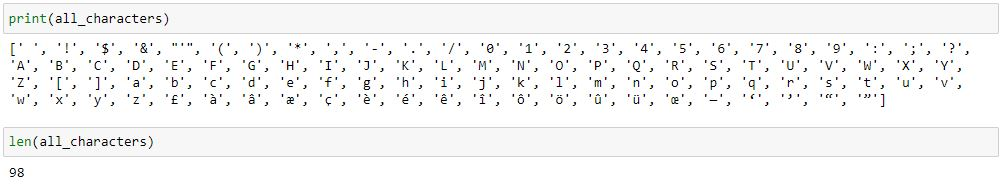
\includegraphics[width = 1.0\textwidth]{Images/single_chars.JPG} % enter the filename here
		\caption{Unique Individual Characters}
		\label{fig:single-chars-all}
	\end{center}
\end{figure}

\begin{figure}[H]
	\begin{center}
		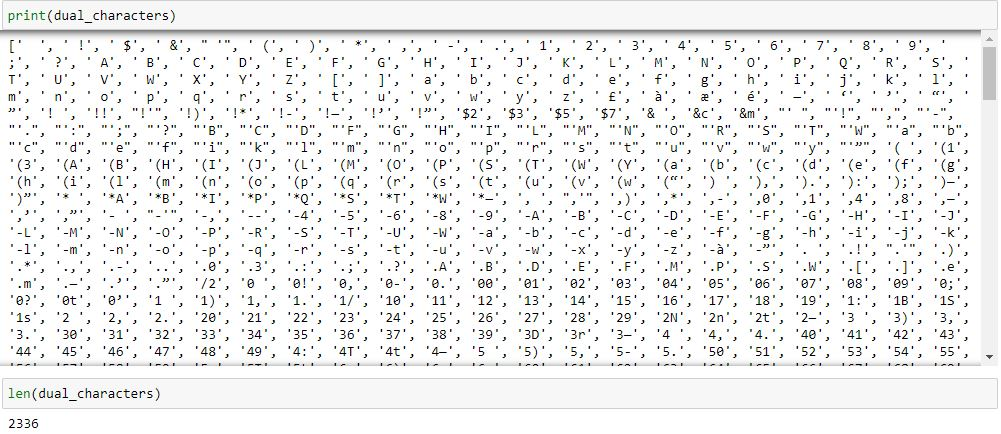
\includegraphics[width = 1.0\textwidth]{Images/dual_chars.JPG} % enter the filename here
		\caption{Unique Dual Character Sets}
		\label{fig:dual-chars-all}
	\end{center}
\end{figure}


\section{Modeling and Training}
\label{sec:modeling}

Now, we have already defined the libraries we would be using in the introduction \ref{sec:python-tools}. Now, let us continue with the overall structure and how we trained our model.
There will be 3 major tasks in this section.

\begin{itemize}
    \item Generating a list of unique single and dual character lists.
    \item Creating a probability distribution for single and dual character sets for each novel.
    \item Generate Log Probabilities and use the equations in \ref{sec:custom-bayes-implementation} into our model.
\end{itemize}
\vspace{0.5cm}

\begin{code}
\label{code:data-split}
\begin{minted}[frame=single,framesep=10pt]{python}
def data_split_custom(text):
    
    texts = len(text)
    # We are using a sample 80-20 train and test split for our novels. 
    split = int(0.8 * texts)
    return text[:split], text[split+1:]
\end{minted}
\caption{Our Function to Split our data into Train and Test samples for future use}.
\end{code}

\subsection{Log Probability Calculation}
\label{sec:log-probability-code}

In this section, we would be covering how we calculated individual and dual character probabilities for all the novels. In the first case of individual probabilities, a simple list works for each novel, yet however, for dual character probabilities, an n*n matrix, which is known as the Transition Matrix, mentioned in the section \label{sec:discrete-space-markov-chains}, and thus each of the novels would need their own DataFrames with these subsequent probabilities.

\subsubsection{Individual Probabilities}
\label{sec:individual-char-probs}
\vspace{0.5cm}

\begin{code}
\label{code:single-char-prob}
\begin{minted}[frame=single,framesep=10pt]{python}
probs = {}
probs_log = {}
charslen = {}

for file in all_files:
            
    book = open(PATH + file, 'r', encoding = 'utf-8-sig')       
    novel = book.read()
    novel = data_cleaning(novel)
    total_len = len(novel)
    novel_train, novel_test = data_split_custom(novel)
    
    probs[file] = {}
    probs_log[file] = {}
    charslen[file] = {}
    
    for char in all_characters:
        charcount = novel_train.count(char)
        probs[file][char] = charcount/total_len
        #Calculating Log Probabilities for all Novels over individual characters
        if charcount == 0:
            probs_log[file][char] = 0
        else:
            probs_log[file][char] = math.log((charcount)/(total_len))
probs_log_df = pd.DataFrame(probs_log)    
\end{minted}
\caption{Loop generates a DataFrame with Single Character Probabilities}.
\end{code}

With this, we get the following DataFrame, which lists out individual character probabilities within a novel. We have kept 0 as an actual occurrence to ensure dual character probabilities are distinguishable.

\begin{figure}[H]
	\begin{center}
		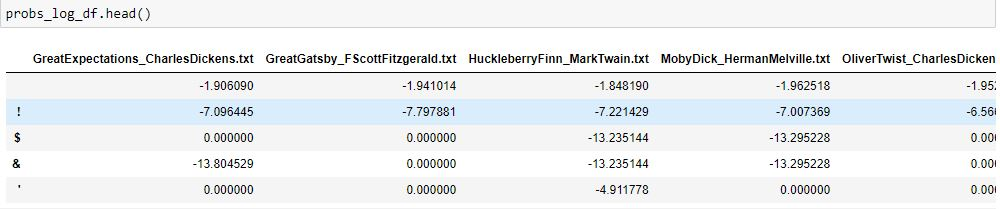
\includegraphics[width = 1.0\textwidth]{Images/single_char_probs.JPG} % enter the filename here
		\caption{Unique Single Character Matrix}
		\label{fig:single-char-prob-matrix}
	\end{center}
\end{figure}

\subsubsection{Dual Probabilities}
\label{sec:dual-char-probs}
\vspace{0.5cm}

\begin{code}
\label{code:transition-matrix}
\begin{minted}[frame=single,framesep=10pt]{python}
for file in all_files:
            
    book = open(PATH + file, 'r', encoding = 'utf-8-sig')
    novel = book.read()
    novel = data_cleaning(novel)
    novel_train, novel_test = data_split_custom(novel)
    counts = np.zeros((len(all_characters), len(all_characters)))
    pairs = zip(novel_train[:-1], novel_train[1:])
    
    for first, second in pairs:
        i = idx[first]
        j = idx[second]
        counts[i,j] += 1
    
    # Laplacian Smoothing
    counts += 1 
    
    #Defining a new DataFrame for each novel. 
    # As an example:
    # GreatExpectations_CharlesDickens is the count of co-occurrences of all characters
    # probs_GreatExpectations_CharlesDickens are the individual probabilities. 
    
    globals()[f"{file[:-4]}"] = counts
    mid_sum = np.sum(counts, axis=1)
    globals()[f"probs_{file[:-4]}"] = pd.DataFrame(counts/(mid_sum.reshape(len(mid_sum),1)), index = idx, columns = idx)
    globals()[f"logs_{file[:-4]}"] = pd.DataFrame(np.log(counts/(mid_sum.reshape(len(mid_sum),1))), index = idx, columns = idx)    
\end{minted}
\caption{Loop generates multiple DataFrames with Dual Character Probabilities}.
\end{code}

We learned about Laplacian Smoothing in the section \ref{sec:laplace-smoothing}. This is where it is extremely important to implement to avoid any data loss within dual character occurrences. The code \ref{code:transition-matrix} results in individual log and normal transition matrices. The names of each of the matrices are as follows. And after that, is an example of what the transition matrix for \textcite{great_expectations} would look like.

\begin{itemize}
    \item logs\textunderscore GreatExpectations\textunderscore CharlesDickens/ probs\textunderscore GreatExpectations\textunderscore CharlesDickens
    \item logs\textunderscore GreatGatsby\textunderscore FScottFitzgerald/ probs\textunderscore GreatGatsby\textunderscore FScottFitzgerald
    \item logs\textunderscore HuckleberryFinn\textunderscore MarkTwain/ probs\textunderscore HuckleberryFinn\textunderscore MarkTwain
    \item logs\textunderscore MobyDick\textunderscore HermanMelville/ probs\textunderscore MobyDick\textunderscore HermanMelville
    \item logs\textunderscore OliverTwist\textunderscore CharlesDickens/ probs\textunderscore OliverTwist\textunderscore CharlesDickens
    \item logs\textunderscore PridePrejudice\textunderscore JaneAusten/ probs\textunderscore PridePrejudice\textunderscore JaneAusten
    \item logs\textunderscore SherlockHolmes\textunderscore ArthurDoyle/ probs\textunderscore SherlockHolmes\textunderscore ArthurDoyle
    \item logs\textunderscore SignOfTheFour\textunderscore ArthurDoyle/ probs\textunderscore SignOfTheFour\textunderscore ArthurDoyle
\end{itemize}

\begin{figure}[H]
	\begin{center}
		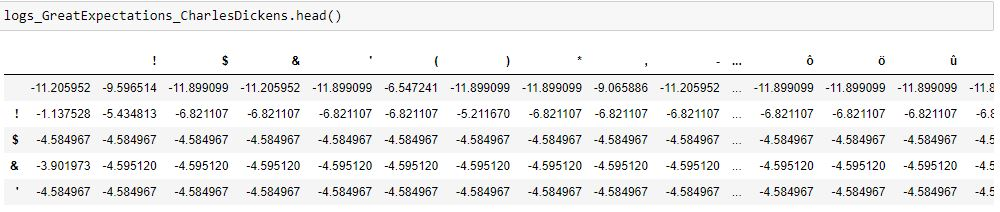
\includegraphics[width = 1.0\textwidth]{Images/transition_matrix.JPG} % enter the filename here
		\caption{Transition Matrix over Novels}
		\label{fig:dual-char-transition-matrix}
	\end{center}
\end{figure}

\textbf{Please Note: Since these are individual transition matrices, each novel in our dataset has a custom DataFrame. Now until this step, the entire code is reproducible over any given text and we can input any novels to generate it. However, the testing phase would be quite customized based on the testing text we choose, with further information in the section \ref{sec:results}}. 

\subsection{Custom Bayes' Rule Code}
\label{sec:code-custom-bayes-markov}

Now with this section, we shall finally implement the theory we studied and derived a final equation in the section \ref{sec:custom-bayes-implementation} with the derived equation \ref{eq:final_custom_bayes}.
\vspace{0.5cm}

\begin{code}
\label{code:final-custom-bayes}
\begin{minted}[frame=single,framesep=10pt]{python}
custom_MarkovChain = np.empty(len(all_files))
for i, file in enumerate(all_files):
    custom_MarkovChain[i] = probs_log_df[file].sum()
    
#With reducing the maximum of the entire model, we are regularizing the entire model.
custom_MarkovChain = custom_MarkovChain - custom_MarkovChain.max()

MarkovChain_Train = pd.DataFrame(data=custom_MarkovChain).T
MarkovChain_Train.columns=all_files    
\end{minted}
\caption{A 1*n DataFrame with final individual book log probabilities}.
\end{code}

With this, we get the following regularized log probabilities for each novel.

\begin{figure}[H]
	\begin{center}
		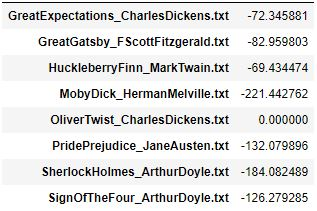
\includegraphics[width = 0.5\textwidth]{Images/markovchain_custom.JPG} % enter the filename here
		\caption{Markov Chain Probabilities}
		\label{fig:custom-markov-chain-probs-final}
	\end{center}
\end{figure}


\section{Testing and Results}
\label{sec:results}

Finally, when we go above and go through the code \ref{code:data-split}, there is a train and a test split. We use this function to create the test data set again, and then generate the log probabilities over the test data from our train data, predicting the closeness of authors with their actual work.

For our test, we shall only be focusing on two tests. It can be increased and changed by re-running the code, which shall be available on GitHub. 

Let us go over the process of testing our code. First, in order to test, we re-define the test pairs from the testing dataset. Please note, that there are way more efficient ways to perform this testing task, but since we are short on time, we are working with individual variables instead of a dynamic variable selection, as will be seen in the code 
\vspace{0.5cm}

\begin{code}
\label{code:testing-data-load}
\begin{minted}[frame=single,framesep=10pt]{python}
book = open(PATH + 'GreatExpectations_CharlesDickens.txt', 'r', encoding = 'utf-8-sig')
novel = book.read()
novel = data_cleaning(novel)
_, greatexp_test = data_split_custom(novel)

test_pairs = set(zip(greatexp_test[:-1], greatexp_test[1:]))
\end{minted}
\caption{Variable greatexp_test used for generating test set}.
\end{code}

Our test pairs look like this:

\begin{figure}[H]
	\begin{center}
		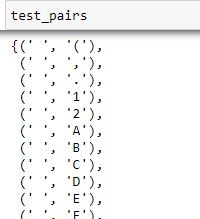
\includegraphics[width = 0.4\textwidth]{Images/test_pairs.JPG} % enter the filename here
		\caption{Test Dual Character Pairs}
		\label{fig:test-char-pairs}
	\end{center}
\end{figure}
\vspace{0.5cm}

\begin{code}
\label{code:testing-matrix-gen}
\begin{minted}[frame=single,framesep=10pt]{python}
#These variables are listed as abbreviations of the novel and the author name combined.
    
GECD_test = 0
GGFSF_test = 0
HFMT_test = 0
MDHM_test = 0
OTCD_test = 0
PPJA_test = 0
SAAD_test = 0
STFAD_test = 0

test_df = MarkovChain_Train.copy()

for first, second in test_pairs:
    
    GECD_test += logs_GreatExpectations_CharlesDickens.loc[first, second]
    GGFSF_test += logs_GreatGatsby_FScottFitzgerald.loc[first, second]
    HFMT_test += logs_HuckleberryFinn_MarkTwain.loc[first, second]
    MDHM_test += logs_MobyDick_HermanMelville.loc[first, second]
    OTCD_test += logs_OliverTwist_CharlesDickens.loc[first, second]
    PPJA_test += logs_PridePrejudice_JaneAusten.loc[first, second]
    SAAD_test += logs_SherlockHolmes_ArthurDoyle.loc[first, second]
    STFAD_test += logs_SignOfTheFour_ArthurDoyle.loc[first, second]

test_df['GreatExpectations_CharlesDickens.txt'] = GECD_test
test_df['GreatGatsby_FScottFitzgerald.txt'] = GGFSF_test
test_df['HuckleberryFinn_MarkTwain.txt'] = HFMT_test
test_df['MobyDick_HermanMelville.txt'] = MDHM_test
test_df['OliverTwist_CharlesDickens.txt'] = OTCD_test
test_df['PridePrejudice_JaneAusten.txt'] = PPJA_test
test_df['SherlockHolmes_ArthurDoyle.txt'] = SAAD_test
test_df['SignOfTheFour_ArthurDoyle.txt'] = STFAD_test

max_test_coef = max(GECD_test, GGFSF_test, HFMT_test, MDHM_test, OTCD_test, PPJA_test, SAAD_test, STFAD_test)

test_df = test_df - max_test_coef
test_df.T
\end{minted}
\caption{Semi-Reproducible Testing Process}.
\end{code}

When tested alongside with two books - \ref{sec:great-expectations} and \ref{sec:moby-dick}, give us some very interesting results. 

\begin{figure}[H]
	\begin{center}
		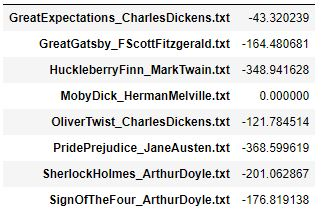
\includegraphics[width = 0.5\textwidth]{Images/testing_greatexp.JPG} % enter the filename here
		\caption{Great Expectations Testing Final Markov Chain Results}
		\label{fig:test-great-expectations}
	\end{center}
\end{figure}

\begin{figure}[H]
	\begin{center}
		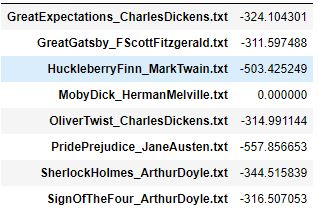
\includegraphics[width = 0.5\textwidth]{Images/testing_mobydick.JPG} % enter the filename here
		\caption{Moby Dick Testing Final Markov Chain Results}
		\label{fig:test-moby-dick}
	\end{center}
\end{figure}

Now, from \ref{fig:test-great-expectations}, we see that our model is predicting Great Expectations to be the second highest value. Moby Dick has the lowest value in the predicted value when we incorporate the equation \ref{eq:custom-test-results}. However, when we look at the prediction for Moby Dick, we get a very well-defined value whereas all other books are quite distant from the value for Moby Dick when it was trained over itself. However, this is just the first iteration, and in case we began training the model over a Gradient Descent model, in order to reduce the probabilities over a given sequence, we could have observed better results. But since we do not train over Markov Chains, this first iteration also gives us very good results.

We shall conclude our dissertation in the next chapter.




\chapter{Conclusion and Possibilities}
\label{cha:conclusion}

In this dissertation, a simple algorithm, \ref{cha:markov-chains} along with a derivation of \ref{cha:bayes}, to reach a new custom model namely \ref{cha:markov_chain_text}, which we implemented using a very simple dataset of novels acquired from \textcite{project-gutenburg}. Markov Chains are very useful in classifying texts in books as they have a very unique process of identifying specific features. 

In general, the most widely used implementation of Markov Chains with books is using words that we went through in the section \ref{sec:token_words} in chapter 5. This works really well when words act as nodes of the Markov Chain and edges are then the probabilities. However, we found that working with characters was a bit tricky, which was quite evident in the results as well, where we saw a weird result for one of the tests predicting another book and placing the original book and author in second place. 

Now, we could also have worked with a true neural network model, as Markov Chains are an example of a probability-based completely connected layer. In case we were to increase layers of modeling in our training, introducing new or existing algorithms, we could have seen better results as well. In the near future, this same project can be advanced by implementing newer layers of classification algorithms such as Random Forest Classifier, Gradient Descent Classifier, etc. The performance could also have been wildly improved if we tried to use a different variation of statistical technique, such as logarithm along with square-root or cube-root of the original probabilities, but that is a reason to speculate the probabilities. 

Finally, I would like to mention that characters were a chosen form, in order to find a relationship between different character occurrences rather than words or subwords as this way, I was able to both reduce computational requirements and keep the complexity at a minimal value.





% ------------------------------------------------------------------------------
% Reference list
% ------------------------------------------------------------------------------
\addcontentsline{toc}{chapter}{References}
\renewcommand\bibname{References}
\printbibliography

% ------------------------------------------------------------------------------
% Appendices
% ------------------------------------------------------------------------------
% --------------------------------------------------
% Appendices
% --------------------------------------------------
\appendix
\chapter{Appendix Chapter}

A lot of research has gone into improving textual models with Neural Networks and in some ways, Markov Models were the stepping stones for their interconnected layers. Following are some links that could be a good read for anyone wishing to delve deeper into this research.

Please note that these links are not references, and thus, have been kept separate from the Bibliography section. This appendix is added so as to help in further research in the topic if needed.

Complete Code Repository for this Dissertation: \href{https://github.com/saranshbh/Uni-of-Leeds-22-Dissertation}{GitHub}.

Markov Chains with Neural Networks: \href{https://www.tnt.uni-hannover.de/papers/data/1276/Awiszus_Markov_Chain_NNs.pdf}{Click Here}

Hidden Markov Models with Neural Networks: \href{https://arxiv.org/abs/2102.11038}{HM Models with CNNs}



\end{document}